% !TeX root = ../main-english.tex
% !TeX spellcheck = en-US
% !TeX encoding = utf8
% -*- coding:utf-8 mod:LaTeX -*-

%This smart spell only works if no changes have been made to the chapter
%using the options proposed in preambel/chapterheads.tex.
\setchapterpreamble[u]{%
	\dictum[Albert Einstein]{If we knew what it was we were doing, it would not be called research, would it?}
}

\chapter{Reproducible brain state analyses}
\label{chap:k4}

The previous chapter focused on the technical challenges of reproducibility management, especially when applications need to scale to large samples, but it also highlighted readily available, pragmatic strategies to ensure portability and reusability.
A different challenge arises when the to be undertaken analyses are not entirely mapped out from the start, and a research project is exploratory in nature.
This upcoming chapter describes the central data analysis project in this thesis, studying working memory in sequential decision making.
The setup of the exploratory analyses I conducted in this project used best practices and tools from Chapter \ref{chap:k1-rdm-2}, and followed the strategies and the framework outlined in Chapter \ref{chap:k3}.
Corresponding project directories leave a transparent digital provenance trace for future reuse, and analyses are portable across infrastructures.
At the time of writing, the work presented in this chapter is being prepared as a research article.

\section{Project outline}

%\section{Theoretical background}
%
%
%In natural settings, value-based decisions under risk often have to be made without visual presence of competing alternatives.
%Do I commit to buying the red bicycle in the store I'm currently in, or should I return to the previous bike shop and pick the blue one?
%Do I want to rent the flat I viewed last Sunday, or the apartment I saw on Tuesday?
%In such situations, relevant properties of alternative options such as their subjective value have to be encoded, held in working memory through a maintenance (or ``delay'') period, and retrieved in order to form a categorical choice.
%To understand the neural processes underlying behavior in these situations, the neural activity in the delay period and how it might represent or maintain relevant properties were a focus of research in the last decades, but although several popular theories emerged over time and were either refuted or refined, the field yet lacks a comprehensive understanding \citep{sreenivasan2019and}.
%In the following, I will outline a brief overview of some major theoretical and methodological approaches.\\
%Early neuroimaging and electrophysiology studies suggested persistent neural activity (``spiking'') in specific brain areas during delay periods as a mechanism of working memory maintenance \citep{goldman1995cellular}.
%Sustained, above-baseline activity that starts during a sample presentation, lasts through the memory delay, and returns to base line activity after a response were found in prefrontal regions in human \citep[e.g.,][]{courtney1997transient} and non-human primates \citep[e.g.,][]{fuster1971neuron, funahashi1989mnemonic, miller1996neural}.
%And single-cell recordings from the prefrontal cortex in monkeys unveiled that individual neurons display activity that is selective to specific task-relevant aspects, such as task rules, spatial location, or stimulus features \citep{white1999rule, wallis2001single}, suggesting the existence of neurons that uphold working memory content with a fixed selectivity for certain properties.
%Others have pointed out, however, that persistent spiking in prefrontal areas could reflect a variety of other different processes, including decision making \citep{curtis2010beyond} or anticipation of the probe \citep{nobre2011attention}, that the high metabolic costs of action potentials is too energetically expensive to hold information in a spiking form \citep{attwell2001energy}, and that distractor tasks are able to remove the persistent activity without an impact on later retrieval, questioning its role in working memory maintenance \citep{larocque2013decoding, lewis2015neural}.\\
%The idea of neural selectivity to specific task-aspects was refined in the adaptive coding framework \citep{duncan2001adaptive}:
%Instead of a persistent, fixed selectivity, it postulates that neural responses are temporarily tuned to the particular task. This theory was able to explain how a recording of spiking activity in the same group of neurons relates to object information in one task but a location distinction in the next task \citep{duncan2001adaptive}.
%\citet{mongillo2008synaptic} proposed a highly influential theory according to which short-term neural plasticity changes are the underlying mechanism of working memory maintenance.
%Working memory maintenance is established via increased residual calcium levels at the presynaptic terminals of neurons, which causes a short-term synaptic facilitation, akin to synaptic weights that link neurons coding for a working memory item.
%With this facilitation, the memory can be transiently held for about 1s without enhanced spiking activity in a network of neurons.
%Building up on this theory,  \citet{stokes2015activity} proposed the dynamic coding framework, in which working memory is mediated by rapid transitions in such ``activity silent'' neural states.
%While these states mediate flexible, context-dependent processing they do not emerge as constant activity and rather as ``hidden states'', appearing as altered response sensitivities of neural networks, established via short-term and long-term synaptic plasticity and temporal functional connectivity changes that influence the response to stimuli.
%An explanation why spiking activity is nevertheless found during delay periods comes from findings that a task-irrelevant read-out or ``ping'' signal is able to reactivate the neural assembly \citep{trubutschek2017theory}.
%This raises the possibility that previous findings of neuronal spiking might have been similar readouts from an activity silent population after task-irrelevant non-specific inputs \citep{wolff2017dynamic}.
%Alternatively, \citet{fiebig2017spiking} proposed that occasional spiking of memory-encoding neurons is needed to refresh the activity-silent states.\\
%The idea that distributed representations that selectively favor information relevant to the current task emerge on the level of neural populations was central in other theories as well.
%\citet{rigotti2013importance} proposed the concept of mixed selectivity, in which information is distributed across neurons through non-linear and high-dimensional representations even when it is not observable in individual cells.
%The rise of multivariate methods such as decoding analyses gave way to thorough investigations of distributed neural patterns.
%\citet{king2014characterizing} formalized this with the temporal generalization method.
%In this method, several classifiers are trained on different time slices of training data each, and tested on all available times in the test data, thus revealing whether the neural code is stable or dynamically evolving.
%Interestingly, studies decoding working memory content found that decodable patterns can be non-stationary (Figure \ref{fig:dynamiccoding}).
%\citet{meyers2008dynamic} decoded object categories from electrophysiological data, and yielded worse decoding the more temporally distant training and testing times slices were apart.
%\citet{stokes2013dynamic} used temporal cross-correlation analyses to show that population responses in the prefrontal cortex evolve during a memory delay.
%These representations of task-relevant stimulus information in temporarily and spatially distributed activity across neurons were termed dynamic population coding \citep{sreenivasan2014revisiting}.\\
%A prominent theory in line with non-stable representations is that cognitive processes evolve through different so-called \textit{brain states} as dynamic neural trajectories \citep{buonomano2009state}.
%These trajectories emerge by conceptualizing neural responses as vectors in an N-dimensional space that evolves over time:
%The axis of the high-dimensional space correspond to measurements, such as raw or transformed data from M/EEG sensors or \gls{fMRI} voxels.
%The neural trajectories emerge by tracing the activity on these axes over multiple time points.
%
%%\begin{figure}
%%	\centering
%%	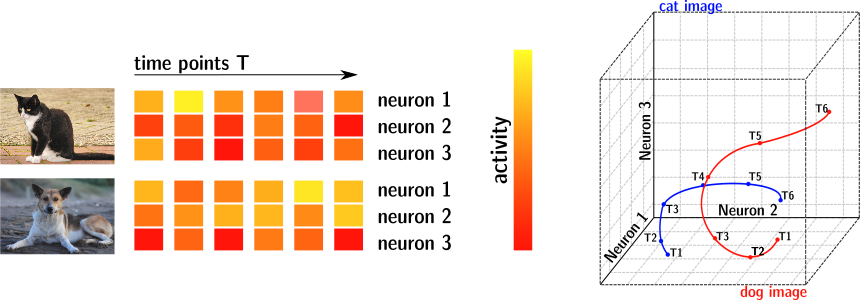
\includegraphics[width=0.5\textwidth]{memento/dynamic_coding.png}
%%	\caption[The dynamic coding framework]{A schematic illustration of dynamic coding in neural populations. The left side depicts a population of three neurons (squares), and their activity (color) over six time points time in response to two visual stimuli. The neural code in this population is not stationary, but dynamic: Each stimulus evokes a distinct response, but within this response, each time point has a different pattern of neural activity, too. By conceptualizing activity patterns over time as vectors, these patterns can be visualized in a high-dimensional space (right). This space has as many dimensions as there are measurement sites (e.g., neurons, sensors, voxels, or electrodes). Dynamic population codes create trajectories through this space. Adapted from \citep[][Fig. 2]{meyers2018dynamic}.}
%%	\label{fig:dynamiccoding}
%%\end{figure}
%
%To bridge the gap to theories of activity silent states, these neural responses are not solely determined by external stimuli, but also internal state changes of the network, such as the strength of synaptic connections, or excitatory or inhibitory influences from other networks \citep{buonomano2009state}.
%Distinct neural states were often hypothesized to reflect steps in mental processing \citep[e.g.,][]{seidemann1996simultaneously}.
%\citet{muhle2021hierarchy}, for example, proposed a hierarchy of functional states in working memory, with items relevant for a pending decision in the most active state, and items relevant only for later use in latent states.
%But studies were also able to extract external stimulus information from the trajectories of transient states, for example odors \citep{mazor2005transient}.
%The study of these neural states and their transition has emerged as its own field, employing multivariate methods such as decoding across neural populations, hidden Markov models (HMMs) to model ensemble activity as a sequence of constantly shifting neural states \citep{rainer2000neural}, or functional alignment \citep{haxby2011common} to find common representations across idiosyncratic neural responses.
%In parallel, dimensionality-reduction gained popularity in analyzing neural population data \citep{cunningham2014dimensionality}.
%The underlying assumption to this approach is that the measured neural activity is too complex compared with the few relevant task or stimulus aspects that require encoding, and that the neural signal of interest must be embedded in a subspace of the high-dimensional neural space.
%\citet{santhanam2009factor} employed a decoding approach based on factor-analysis to reduce noise in high-dimensional neural recordings to improve the performance of neural prostheses, which otherwise suffered from the neural variability introduced by changes in attentional state or wakefulness.
%The term ``effective dimensionality'' of population activity emerged in the literature to identify shared components of collective dynamics that reflect task variables \citep{jazayeri2021interpreting}.
%\citet{murray2017stable} used \gls{pca} on electrophysiology recordings acquired from primate prefrontal cortex during a working memory task, and found a lower-dimensional subspace in the high-dimensional state space in which stimulus representations were stable across the cue and delay epochs.
%\citet{machens2010functional} likewise used \gls{pca} in a working memory task where non-human primates compared the frequency of two vibrations to identify a 6-dimensional subspace in which this tactile stimulus information is represented.
%\citet{gallego2017neural} proposed the neural manifold hypothesis.
%In this hypothesis, behavior is controlled by neural modes, patterns of neural population covariance.
%The high-dimensional neural space is confined into a lower dimensional ``manifold'' spanned by these neural modes.
%Dimensionality reduction methods would allow to identify the foundational neural modes that confine population activity, and allow the study of neural population dynamics.
%They further showed that the low dimensional spaces remained stable over multiple years by aligning the manifolds from separate measurements \citep{gallego2020long}.\\

%\section{Working memory maintenance}

Drawing insights from the partial overview of the literature in Chapter \ref{chap:k1}, methods to study working memory have shifted from traditional evoked potentials to computationally intensive processing.
The field has progressed from studying spiking activity in single cells to an implicit consensus that the neural representation of working memory during maintenance is high-dimensional or embedded in a high-dimensional space, time-varying, and spatiotemporal distributed.
But despite the wealth of theories and methodological approaches, the field has not yet converged on a full understanding of working memory.
Recent reviews have begun to point out where findings and standard views fall short to yet explain the mechanisms underpinning working memory \citep{nobre2022opening}, or highlight the inconsistencies in results across studies \citep{pavlov2022oscillatory}.
While studies traditionally focused on the involvement of prefrontal areas due to its involvement in executive control \citep[e.g.,][]{fuster1971neuron, funahashi1989mnemonic, miller1996neural}, many other brain areas have been shown to represent working memory items, too.
In a recent review, \citet{sreenivasan2019and} summarized how single-cell measurements, MEEG, and \gls{fMRI} acquisitions have found increased activity during working memory maintenance throughout the cortex and even some subcortical areas.
\citet{d2007cognitive} also described working memory as an emergent property of functional interactions prefrontal areas and the rest of the brain as opposed to being localized to a single brain region.
And while an often proposed mechanism for the coordination of temporal and spatial population codes are brain oscillations in specific frequency bands \citet[e.g.,][]{roux2014working}, %for example concluded that gamma and alpha band oscillations of groups of neurons are generically involved in the maintenance of sensory-spatial working memory items.
a recent systematic review by \citet{pavlov2022oscillatory} highlighted a prominent lack of agreement across results in experimental studies that reported observations of brain oscillations in working memory tasks.\\
%Decoding approaches can find multiple different working memory items simultaneously in the same neural population \citep{rigotti2013importance}, and in various brain regions \citep{curtis2010beyond}.
In light of variable and even conflicting findings, \citet{nobre2022opening} called for sustained open-mindedness and creativity in researching working memory in a recent reflective piece.
In this exploratory spirit, I conducted the simulations and analyses that will be described in this chapter.
They build up on previous analysis that were conducted on this dataset by \citet{kaiserposter}, who studied the temporal dynamics of working memory maintenance with this dataset, in particular how decision-relevant stimulus features are represented in the delay phase.
My extensions of their analyses connect to the works of \citet{murray2017stable} and \citet{machens2010functional}:
\citet{murray2017stable} found neural subspaces within dynamic population-level activity that showed stable coding for working memory items. They used \gls{pca} to construct low-dimensional subspaces ($k = 1$ or $k = 2$, respectively) in electro-physiological recordings from non-human primates, and projected neural recordings into the subspaces such that the principal components became the axes of a new, lower-dimensional state space. In these subspaces, stable population codes and above-chance decoding accuracies for working memory items in two different working memory tasks arose.
\citet{machens2010functional} similarly used \gls{pca} on high-dimensional electro-physiological data to create a new, lower-dimensional subspace ($k = 6$) based on identified components and interpreted the resulting axes in relation to the experimental decision making task.
In the following, they identified components representing time (``when'') and components representing working memory content (``what'').
Taken together, these studies thus employed dimensionality reduction methods to perform statistical decomposition in a high dimensional ``native neural space'' to project the axes of a task space into subspaces of the native neural space and assigned meaning to them (see Figure \ref{fig:trajectories}).
Yet contrary to \citet{murray2017stable, machens2010functional}, the upcoming analyses do not confine the neural signal to a specific brain area such as the PFC, but attempt to find neural signatures of decision-relevant working memory items across the cortex.
Central to the analyses is also the attempt to use a functional alignment method more commonly used in \gls{fMRI} for  dimensionality reduction.\\
Such an exploratory neuroscientific project faces several challenges.
As outlined in Chapter \ref{chap:k1}, analyses are often multi-stepped.
But repeating the same processing step in all of many different analyses is computationally inefficient.
Furthermore, a large number of analyses makes it difficult to retain an intuitive structure.
When several different analyses are conducted in the same directory, researchers unfamiliar with the project struggle to associate inputs, code, software, and results.
But when different analyses are broken into distinct projects, the disk space demands of the underlying neural data usually multiply.
The distributed nature of the project across several institutions also demanded uncompromising portability.
Common exploratory approaches such as interactive computing or notebooks typically do not fulfill this requirement due to their short-lived and environment-dependent nature.
To overcome these challenges, research data management principles from the previous chapter were applied.
All analyses were setup as portable DataLad datasets.
The project evolution was captured in a linked hierarchy of datasets, starting with a BIDS-standardized raw dataset, continuing with a preprocessed derivative dataset, and spreading into multiple analyses applications based on a common starting point (Figure \ref{fig:outline_memento}).
Analyses were codified into infrastructure-agnostic scripts, and their execution was provenance-tracked to allow for re-computations over the course of the project.
Each individual component in the Figure \ref{fig:outline_memento} below constitutes a self-described entry point to further analyses at a later point in time.

\begin{figure}[H]
	\centering
	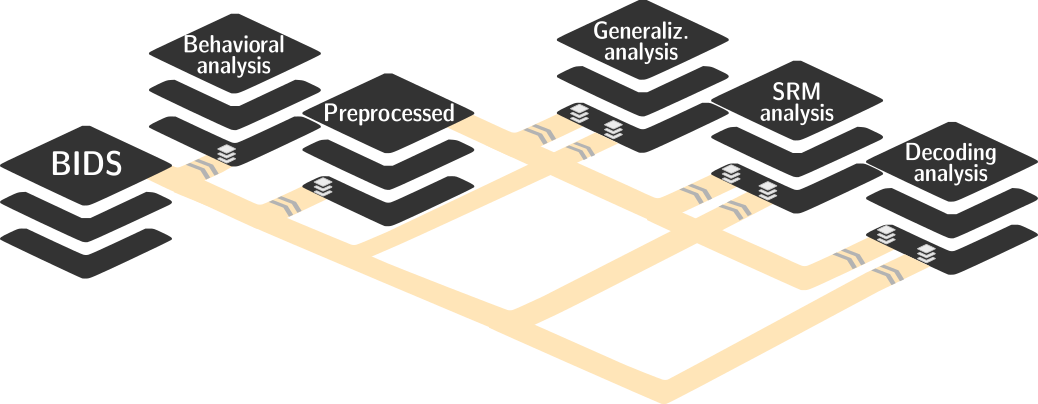
\includegraphics[width=.5\textwidth]{memento/analysis_setup.png}
	\caption[Memento analysis outline]{Project outline as linked DataLad datasets for provenance capture, disk usage reduction, and computational efficiency. A \gls{BIDS}-structured raw dataset is the anchor of all analysis. A common preprocessing pipeline is the basis of three major \gls{meg} analyses. If raw or preprocessed data changes, analysis results can be recomputed automatically.}
	\label{fig:outline_memento}
\end{figure}
%




%\begin{figure}
%	\centering
%	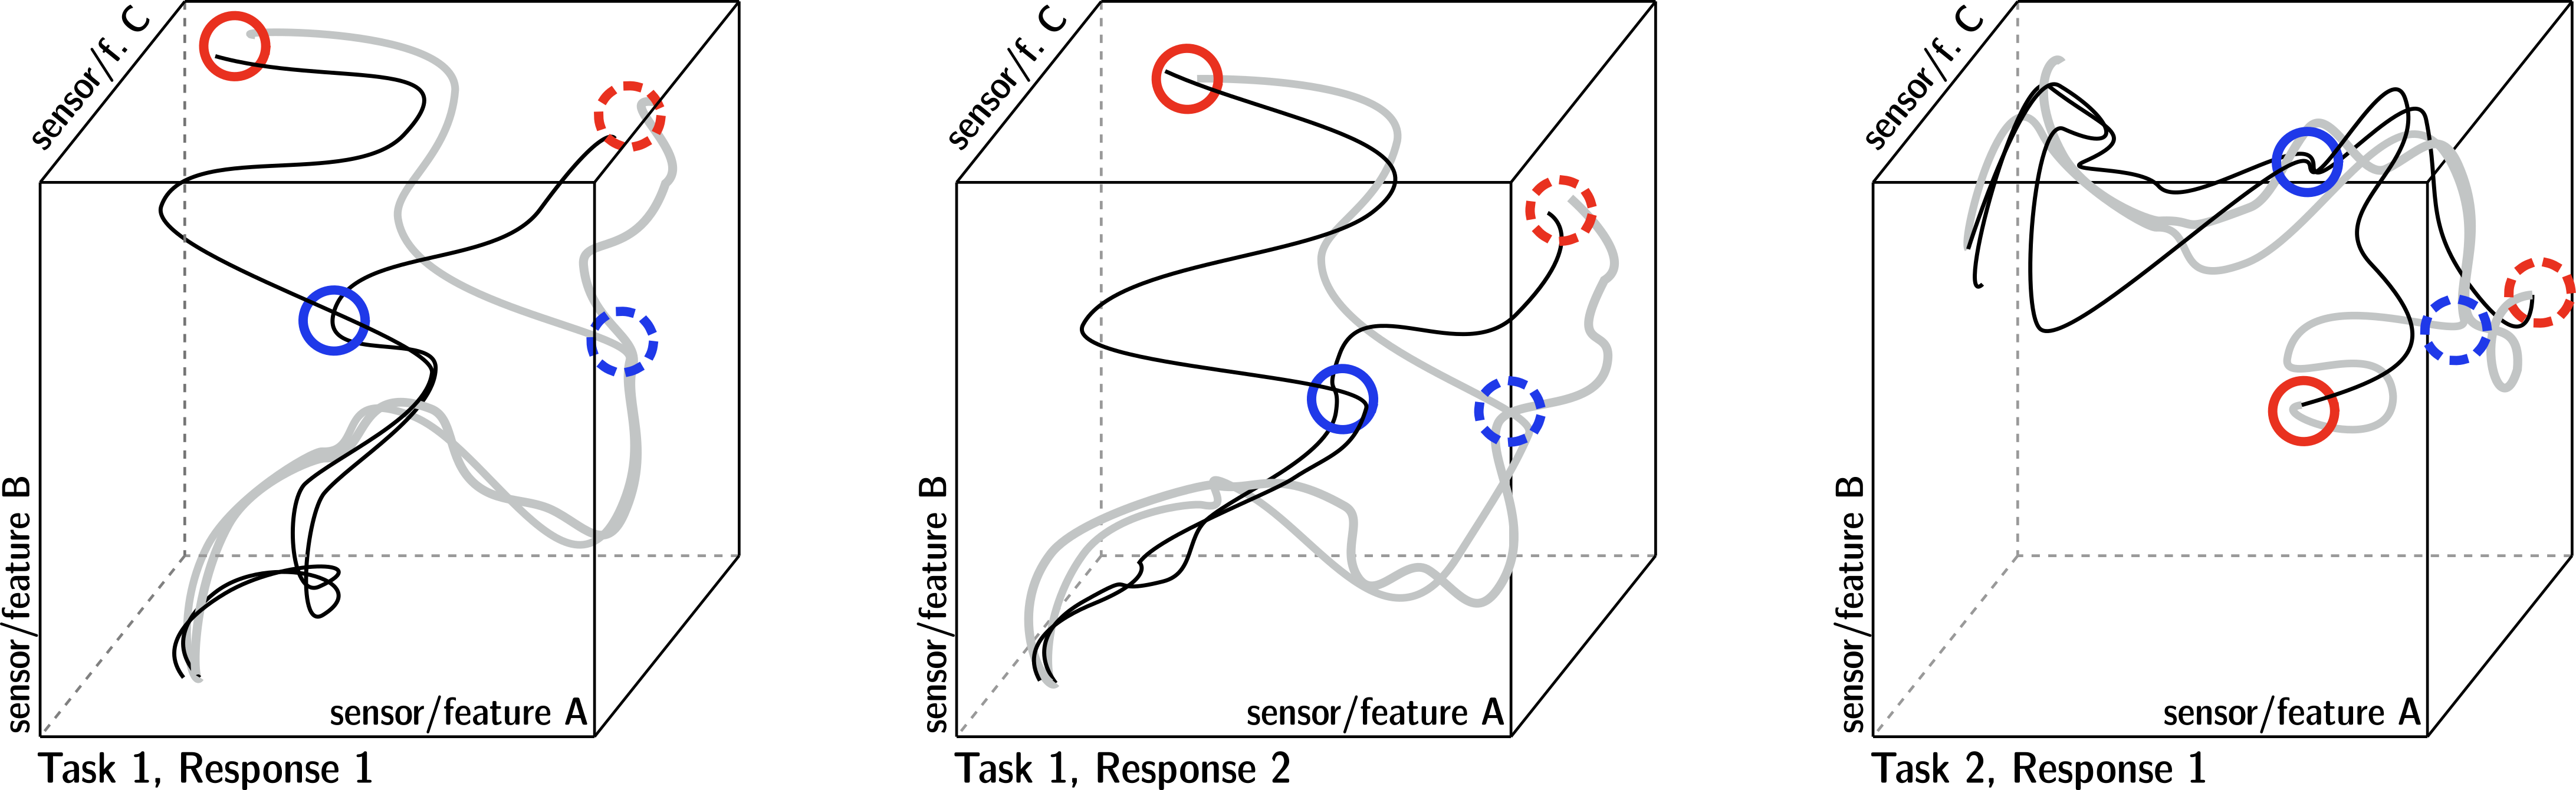
\includegraphics[width=0.5\textwidth]{memento/neural_trajectories_redone.png}
%	\caption[Neural trajectories through state-spaces]{An schematic illustration of neural trajectories through a state-space for two decision alternatives (blue) and two response alternatives (red), for two tasks in a delayed-response-mapping paradigm. Assigning meaning to the axes of the state-space may yield insights about brain states in different experiment conditions. Adapted from Jocham, Krauel, Hanke (unpublished)}
%	\label{fig:trajectories}
%\end{figure}




%The decoding approach, generally speaking, works by identifying patterns that correspond to the experimental task or stimulus in population signals with machine-learning classifiers.


\section{Magnetoencephalograpy (MEG)}

The plurality of analyses in the upcoming sections warrants a more detailed overview of the basic properties, strengths, and weaknesses of data stemming from magnetoencephalography acquisitions.
\gls{meg} is a neuroimaging method to record neural activity from magnetic flux, the total magnetic field passing though a given area.
It is measured on the surface of the head with sensitive detectors, so-called Superconducting Quantum Interference Devices (SQUID) sensors.
The electric currents that give rise to these magnetic fields stem from synchronous inhibitory or excitatory postsynaptic potentials in parallel pyramidal cells in the cortex, mostly those cells in the walls of the cortical sulci.
As the potential differences between soma and axons of neurons form magnetic dipoles, and these cells are perpendicular to the cortical sheet of the gray matter and thus similarly oriented, measurable magnetic fields emerge at the sculp when aggregated across a neuronal population.
The resulting cortical magnetic fields are on the order of $100$-$500$ femtotesla (fT) \citep{hari2017primer}.
Compared to the environmental noise, this is a very weak magnetic field.
Therefore, in addition to active and passive shielding from magnetic or electronic inferences, liquid helium in the \gls{meg} device cools the SQUID sensors to -269°C and allows them to be superconductive.
In this state, a superconducting coil in the SQUID can amplify the magnetic flux, which is picked up by a nearby pickup coil, also called flux transformer.
Three main types of flux transformers exist: magnetometer, axial gradiometer, and planar gradiometer, each with a different sensitivity profile.
An \gls{meg} device can contain different types of flux transformers and the total number of flux transformers is the amount of channels of the \gls{meg} system \citep{puce2017review}.
The analysis of the recorded data then consists of interpreting the resulting topographies given the employed flux transformer.
Typically, \gls{meg} devices contain around 150-300 sensors arranged in a helmet-shaped array that cover the whole human scalp at a frequency of 1000-5000Hz.
The resulting temporal resolution is high compared to neuroimaging methods such as \gls{fMRI} or \gls{pet}.
This makes it a highly suitable modality to study cognitive processes that occur in the range of milliseconds.
The spatial resolution is, however, inferior to the spatial resolution that can be achieved with \gls{fMRI}.
This is aggravated further by the superposition principle of the magnetic field, stating that fields arising from several currents are linear sums of fields generated by each single current.
Thus, the measured signal at the sculp is a mix of multiple magnetic fields, stemming from different sources within and outside the brain that are difficult to disentangle \citep{hari2017primer}.
Data are said to be in ``sensor space'' when read out from the sensors, and in ``source space'' when its cortical sources have been estimated.
All analyses conducted on \gls{meg} data in this chapter were carried out in sensor space.



\section{Study overview}


The data basis of the upcoming analyses stems from a study that investigated how decision-relevant information is retained in working memory using a decision making task with concurrent \gls{meg} acquisition.
The data were acquired as part of the SFB 779 project B16N (``offline value representations in sequential decision making'') at the Otto-von-Guericke University Magdeburg by \citet{kaiser}, and has not been previously published.
%The following study overview adheres to the COBIDAS MEEG reporting guidelines for reproducible MEEG research \citep{pernet2020issues}.


\subsection{Participants}

$N = 22$ right-handed, healthy participants with normal or corrected-to-normal vision were recruited at the Center for Behavioral Brain Sciences and on the University Magdeburg campus.
Their mean age was 26 years, and 10 participants were male.
Handedness was assessed with the Edinburgh Handedness Inventory \citep{oldfield1971assessment}.
Participants gave their informed consent to participate in the study, and received a base monetary compensation in the order of 8€ per hour with a performance-dependent bonus of up to 3€.
Ethics approval was obtained from the University Clinic Magdeburg.

\subsection{Experimental design}

The experiment consisted of 510 trials, grouped into 5 blocks with a variable break in between.
Each trial required a decision between one of two stimulus options, presented as gabor patches on the left and right side of the screen (\cref{fig:memento_trial}).
Importantly, stimulus options were presented in succession, with a delay period through which the decision-relevant properties of the first stimulus had to be retained in working memory.
The number of stripes in the gabor patch encoded the reward magnitude (either 0.5, 1, 2, or 4 points), and the angle of stripes encoded reward probability (either 10\%, 20\%, 40\%, or 80\%).
The more stripes, the higher the reward, and the larger the angle, the higher the probability.
Participants learned these associations in a tutorial prior to the experiment (\cref{fig:memento_tutorial}), and \cref{fig:memento_stim} provides an overview of stimuli.
Stimulus combinations and sequences were selected to fulfill the following requirements:
\begin{enumerate}
	\item To prevent subjects from forming a decision already in the delay period \citep{curtis2010beyond}, the left stimulus never contained the best or worst combination of properties (see Figure \ref{fig:memento_stim}).
	\item In the first option, all magnitude and probability options are shown equally often.
	\item No more than three repetitions of the same probability and magnitude combination occur in the left stimulus.
	\item First and second stimulus are never identical.
	\item The expected values of the left and right stimulus were balanced over the course of the experiment such that left and right options yielded the same reward on average.
\end{enumerate}
Based on these requirements, a fixed reward schedule was generated, and all subjects underwent the same sequence of stimulus combinations.
In approximately half of the trials one of the two stimulus options was clearly favorable, and both its properties (magnitude and probability) were either equal to or greater than that of the other option.
These trials consequently required no integration of stimulus properties to assess which option's value is higher.
In a subset of those trials, called ``no-brainer'' in all following analyses (roughly 10\% of all trials), both magnitude and probability were strictly greater in one of the two options, posing the easiest decision form.
In standard trials, however, stimulus properties were differentially advantageous for the two options.\\
Each trial started with a fixation cross (1000-1900ms, jittered), followed by the first stimulus on the left side of the screen (700ms), a 2000ms delay period through which a central ``or'' was presented, the second stimulus option on the right side (700ms), and a feedback screen.
Once the second stimulus option was displayed, participants chose the left or right option via a button press with the right or left index finger, respectively.
The feedback screen showed both options side by side with a frame around the chosen option, and revealed which option(s) had been rewarded via color coding (red: unrewarded, green: rewarded).
If a decision was not made within 5 seconds, the trial was aborted and participants saw a message to respond faster.
A progress bar at the bottom of the screen tracked gains over time, resulting in a bonus payment whenever it hit a gold target line.
Participants were instructed to maximize their gains and to respond as fast as possible.
Stimulus presentation was controlled by Psychtoolbox \citep{kleiner2007s} running on Matlab 2012b (The Mathworks Company, Natick, MA).
All stimuli were presented on a grey background with a contrast optimized for the MEG recording chamber.
%A photodiode, taped onto the stimulation screen, was used to determine visual stimulus onsets.
%\todo{Add delay}
In total, the experiment lasted approximately 60 minutes.

\begin{figure}
	\centering
	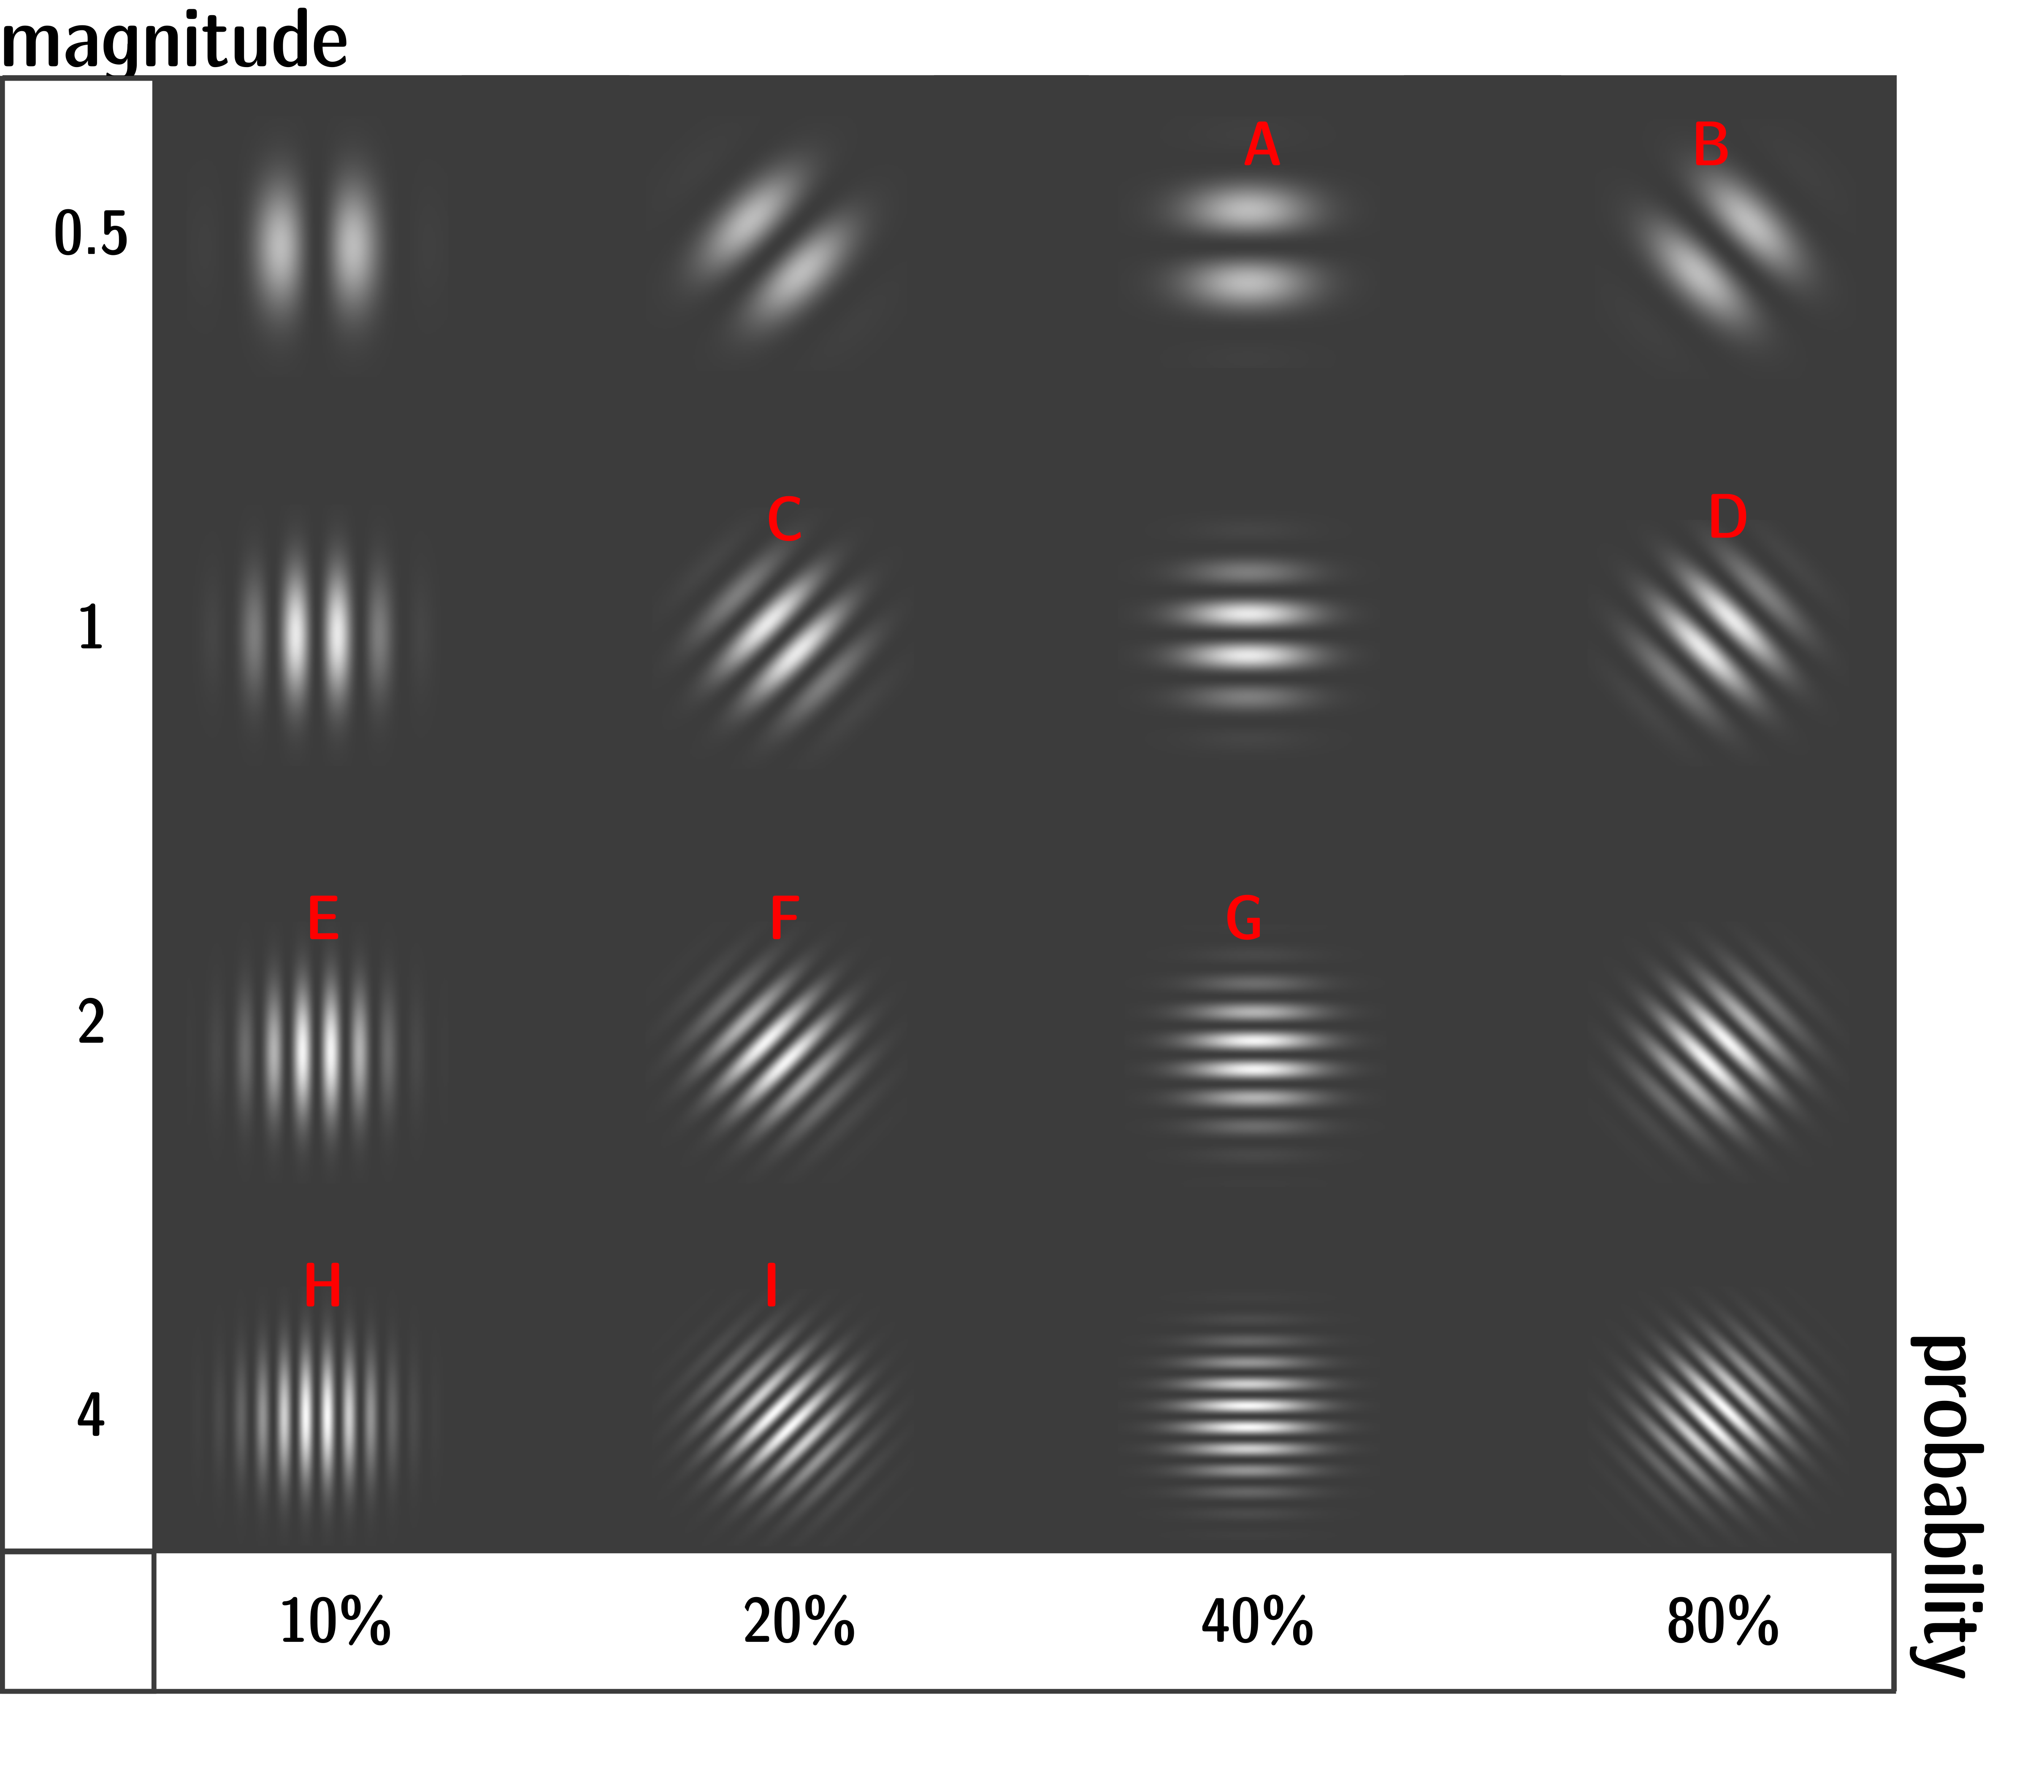
\includegraphics[width=0.5\textwidth]{memento/memento-stimuli.png}
	\caption[Stimulus overview]{Stimulus overview: Gabor patches varied in the number of stripes and their angle, encoding magnitude and probability, respectively. While all presented stimuli were learned in the tutorial, red letters indicate the selection of nine stimulus types used for the left option in the actual experiment. Trials without this annotation were only used intermittent as the right stimulus option to balance the overall expected value between the left and right stimulus option over the course of the experiment.}
	\label{fig:memento_stim}
\end{figure}

\begin{figure}
	\begin{subfigure}{.54\textwidth}
	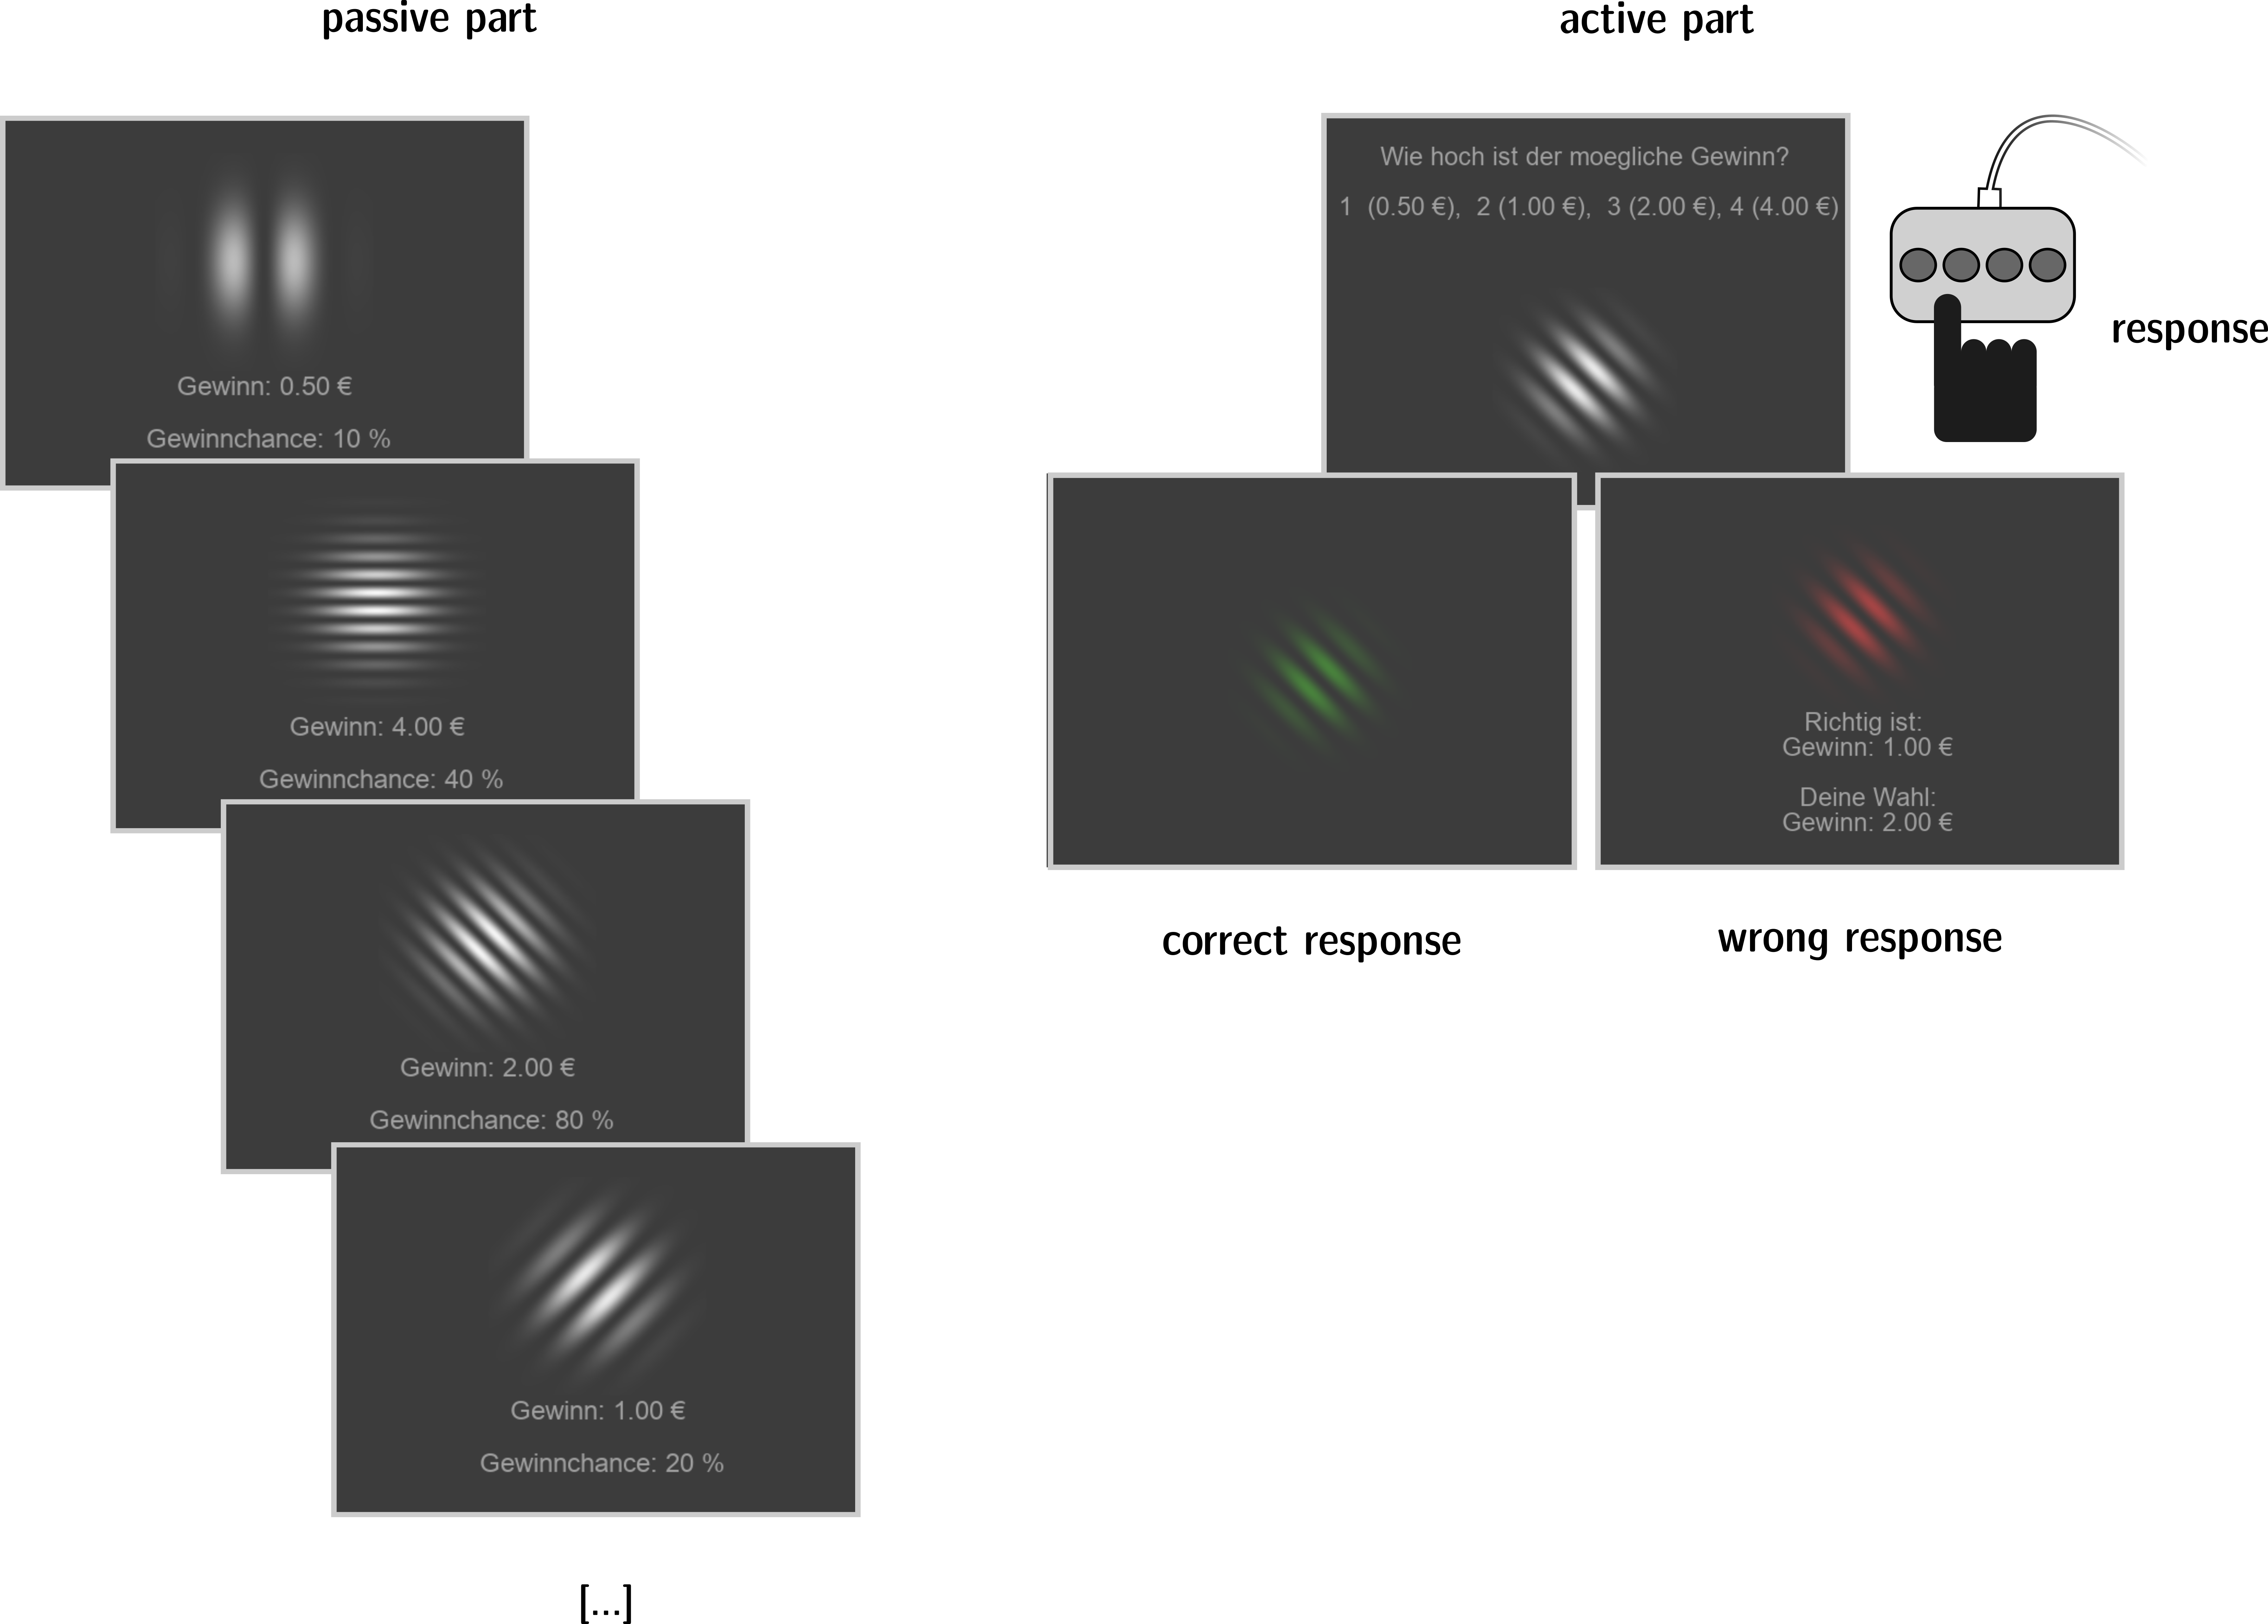
\includegraphics[width=\textwidth]{memento/memento_tutorial.png}
	\caption{Schematic overview of the tutorial.}
	\label{fig:memento_tutorial}
	\end{subfigure}
	\begin{subfigure}{.45\textwidth}
	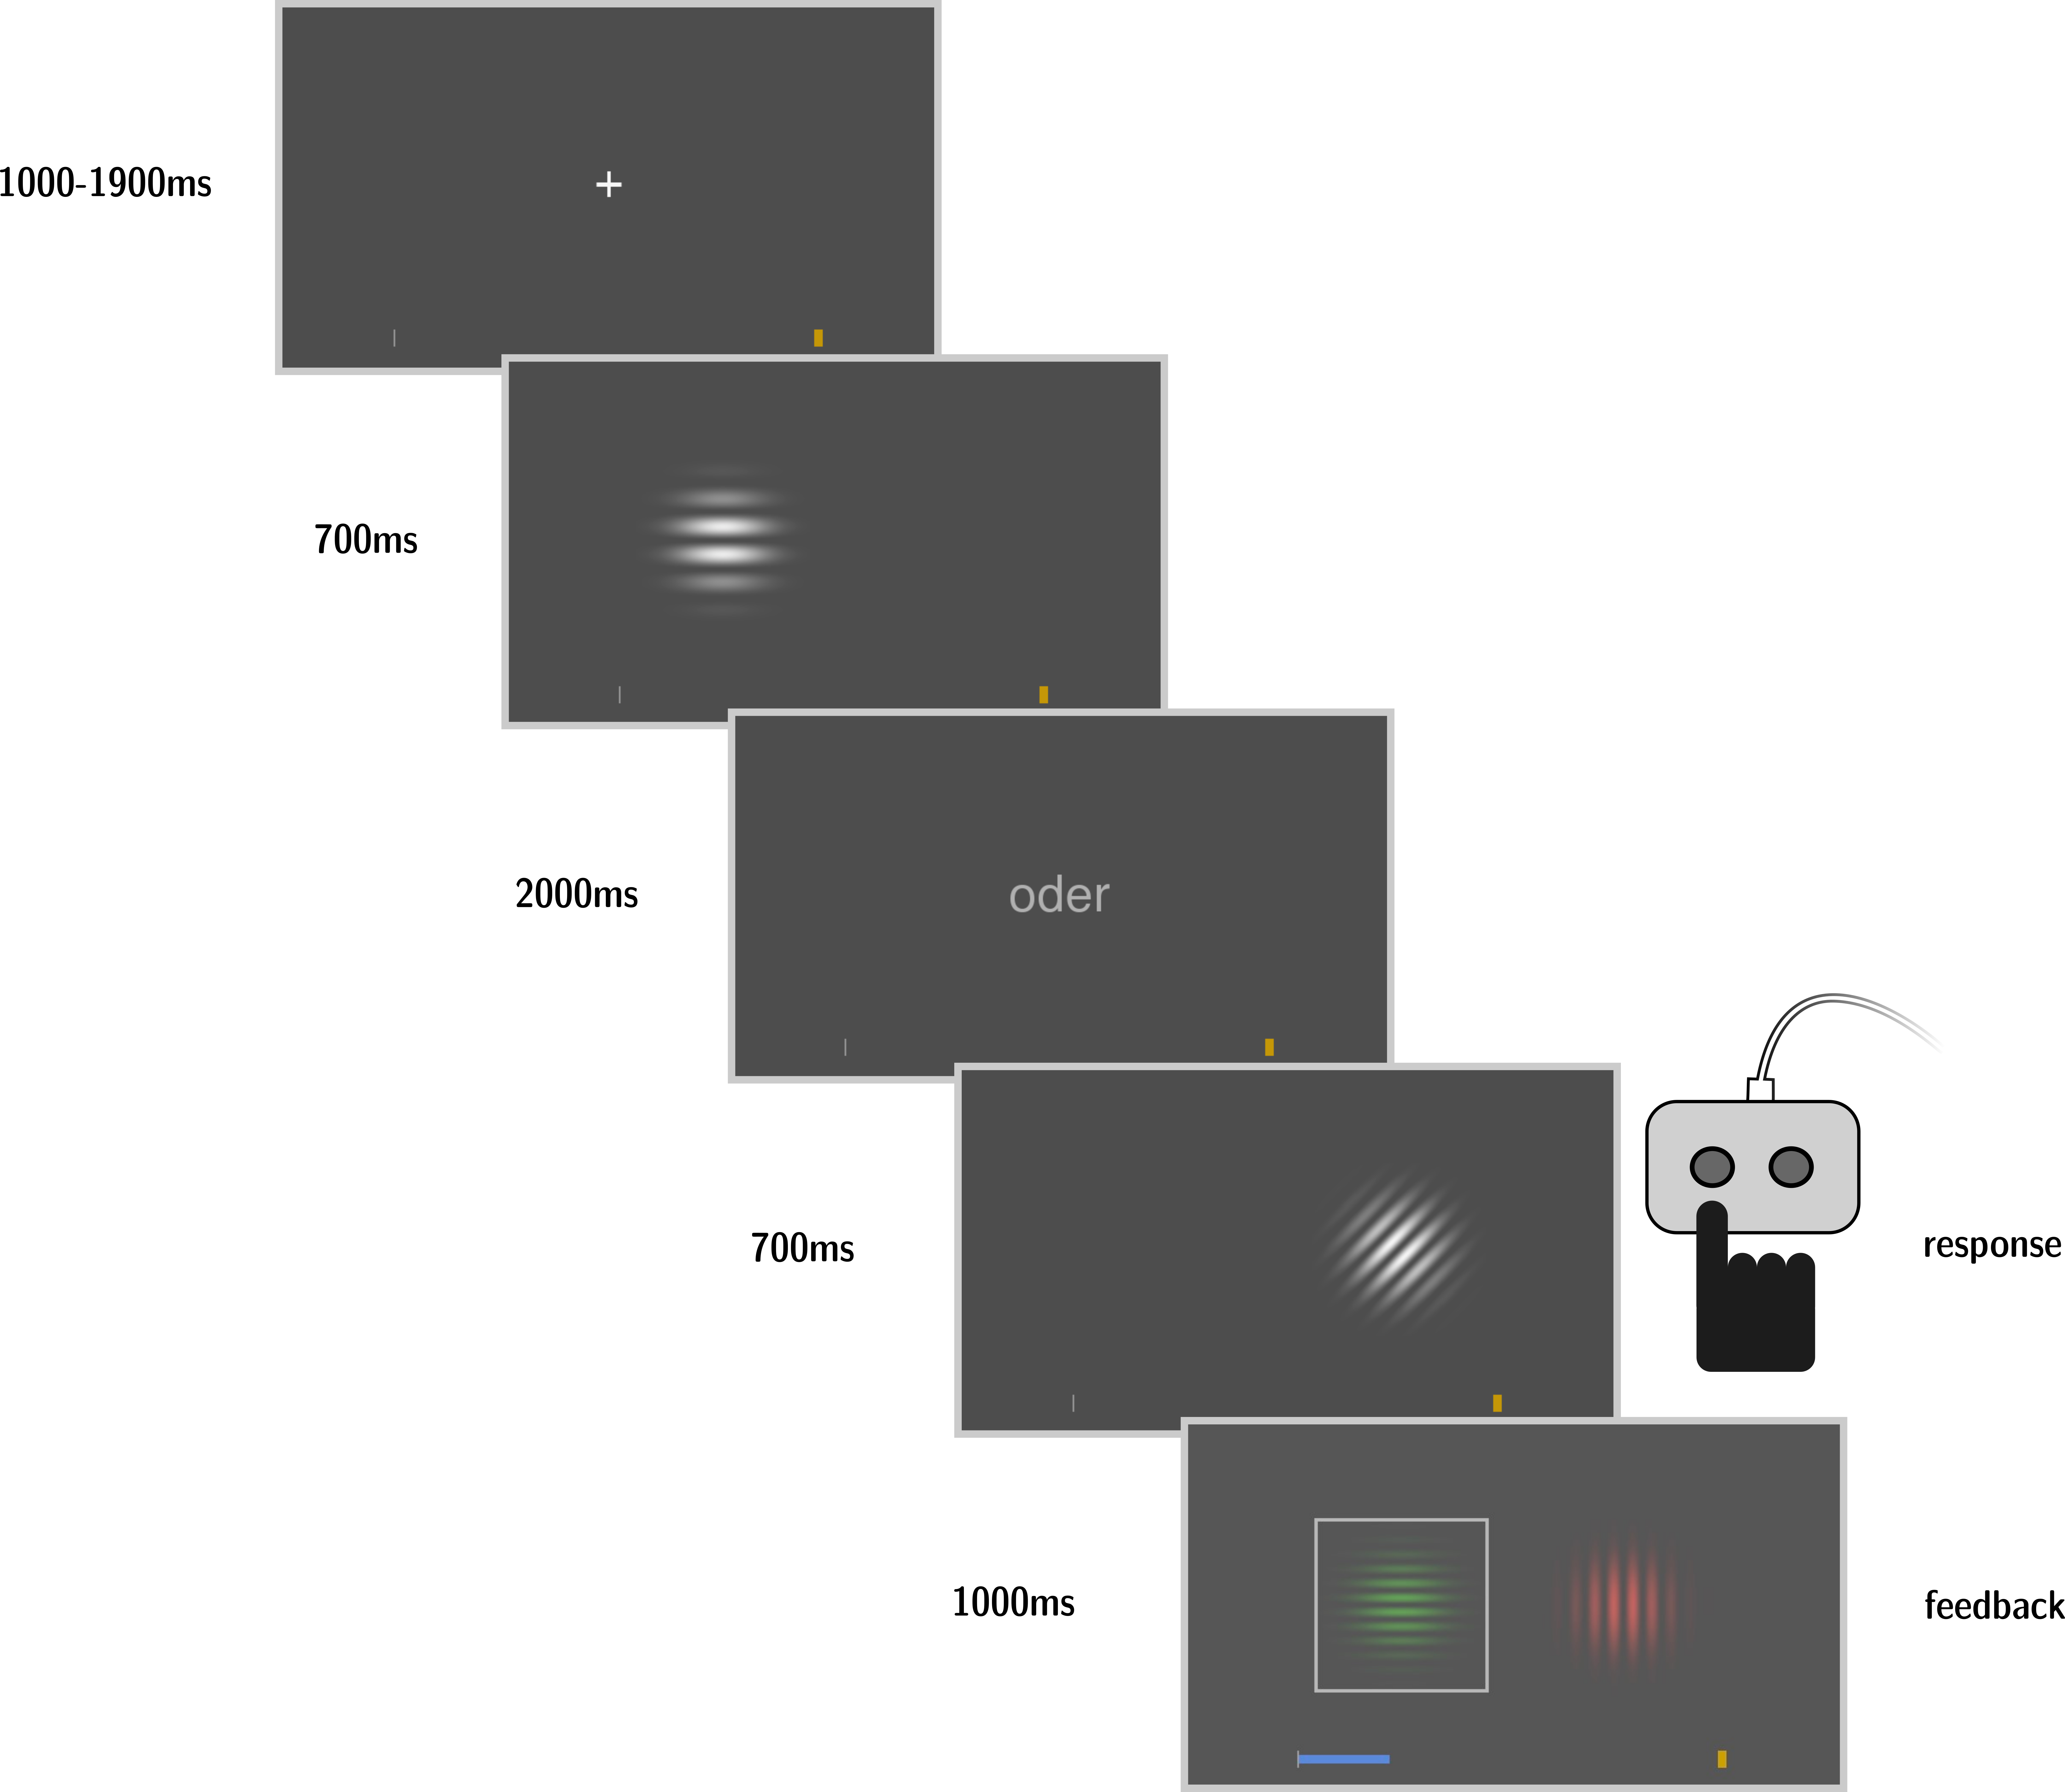
\includegraphics[width=\textwidth]{memento/memento_experiment.png}
	\caption{Schematic overview of a single trial.}
	\label{fig:memento_trial}
\end{subfigure}
	\caption[Memento: Tutorial and trial overview]{Schematic overview of the tutorial (a) and a single trial in the experiment (b).
	The tutorial was split in an active and a passive part.
	In the passive part, participants were presented with a stimulus and how its properties translated to reward magnitude and probability. All possible magnitude and probability combinations were presented twice, and participants controlled the pace. The active part then tested participants' knowledge by presenting a stimulus without the annotation. Based on a text prompt, participants had to report its associated magnitude or probability via button press. They received feedback with a green colored stimulus for a correct response, or, for an incorrect response, a red colored stimulus together with a report of their response versus the true response.
	}
\label{fig:memento}
\end{figure}


\subsection{MEG acquisition}

Following a metal test, MEG data were acquired on an Elekta Neuromag TRIUX System with internal helium recycler and 306 sensors (204 planar gradiometers and 102 magnetometers) in a magnetically shielded room.
Participants were instructed to take a comfortable seating position and sit as still as possible.
The experiment was presented on a screen in a distance of one meter from the sitting participants via a projector with a refresh rate of 60 Hz located outside the MEG recording chamber.
Additional sensors captured confounding biological signals:
Lateral and vertical eye movements and blinks were captured using \gls{eog} surface electrodes on the tori supra- and infraorbitalis and next to the external canthi.
Heartbeat artifacts were recorded with an electrocardiogram (ECG).
Head position indicator coils captured the participants' head movements.
Behavioral responses were registered using an MEG compatible keyboard.
The neural data was recorded at a sampling rate of 1000Hz and active internal shielding (IAS).


\section{Data preparation}

The code I wrote for data preparation, preprocessing and analysis is available as the Python package \texttt{pymento\_meg} from GitHub\footnote{\url{https://github.com/adswa/pymento_meg}} and the Python package index \url{PyPi.org}.
Underlying software packages are listed in Table \ref{tab:software}, and the software environment required for all analyses is also available as Singularity image that can be found alongside the source code (TODO).
\begin{center}
\begin{table}[H]
	\begin{tabular}{ l l l }
		\hline
		Software	& Version 	& Citation \\ \hline
		\texttt{autoreject} 	& 0.4.2 	& \citet{jas2017autoreject} \\
		\texttt{brainiak} 	& custom fork based on v.0.11 & \citet{brainiak} \\
		\texttt{imbalanced-learn} & 0.10.1 & \citet{JMLR:v18:16-365} \\
		\texttt{matplotlib} 	& 3.7.1 	& \citet{Hunter2007} \\
		\texttt{meegkit} 	& 0.1.3 	& \citet{barascud2022} \\
		\texttt{mne-bids} 	& 0.12 		&  \citet{Appelhoff2019} \\
		\texttt{mne-python} 	& 1.4.0		& \citet{Gramfort_MEG_and_EEG_2013} \\
		\texttt{pandas} 		& 2.0.2 	& \citet{The_pandas_development_team_pandas-dev_pandas_Pandas} \\
		\texttt{scikit-learn} & 1.0	 	& \citet{scikit-learn} \\
		\texttt{scipy} 		& 1.10.1 	& \citet{2020SciPy-NMeth} \\
		\texttt{seaborn} 	& 0.12.2 	& \citet{Waskom2021}
	\end{tabular}
	\caption[Overview of software packages]{Overview of internally employed software packages, their versions, and citations.}
	\label{tab:software}
\end{table}
\end{center}

Prior to preprocessing, raw data were restructured to \gls{BIDS} format (v1.4.0) following the \gls{meg} extension of \gls{BIDS} \citep{niso2018meg}.
Several properties of the project made this challenging.
As the acquisition was done in a different institution several years back by \citet{kaiser} and the data had moved locations, crucial metadata was missing from the project files, either because it was lost or not recorded in the first place.
Some information, such as metadata files from the acquisition machine, was acquired post-hoc by emailing the facility in Magdeburg.
Other information, such as some participants' ages or raw data from the handedness acquisitions could not be found.
Furthermore, as \gls{meg} data was acquired on an Elekta Neuromag machine, previous ``raw'' data former analyses were based on was preprocessed in-scanner with Neuromag's propietary MaxFilter\textsuperscript{TM} for motion correction and denoising.
Data that is preprocessed with such a proprietary tool is not an ideal data analysis basis as it can not be easily recomputed without access to the original acquisition machine, which would make a fundamental processing step nontransparent.
However, as only preprocessed files were used previously, it went unnoticed that one of the pristine raw \gls{meg} data files was not copied over from the acquisition machine to the project archive.
With the help of the original authors and a contact at the acquisition facility in Magdeburg it was possible to restore this file from internal archives.
Finally, as the experiment was Matlab-based, behavioral log files were written to proprietary .mat files.
During the transformation to \gls{BIDS}, these log files were transformed into the open TSV format (see Figure \ref{fig:BIDS}).

\section{Preprocessing}
\label{preprocessing}

An overview of preprocessing steps is shown in Figure \ref{fig:preproc}.
The following paragraphs outline individual steps in detail.

\begin{figure}[H]
	\centering
	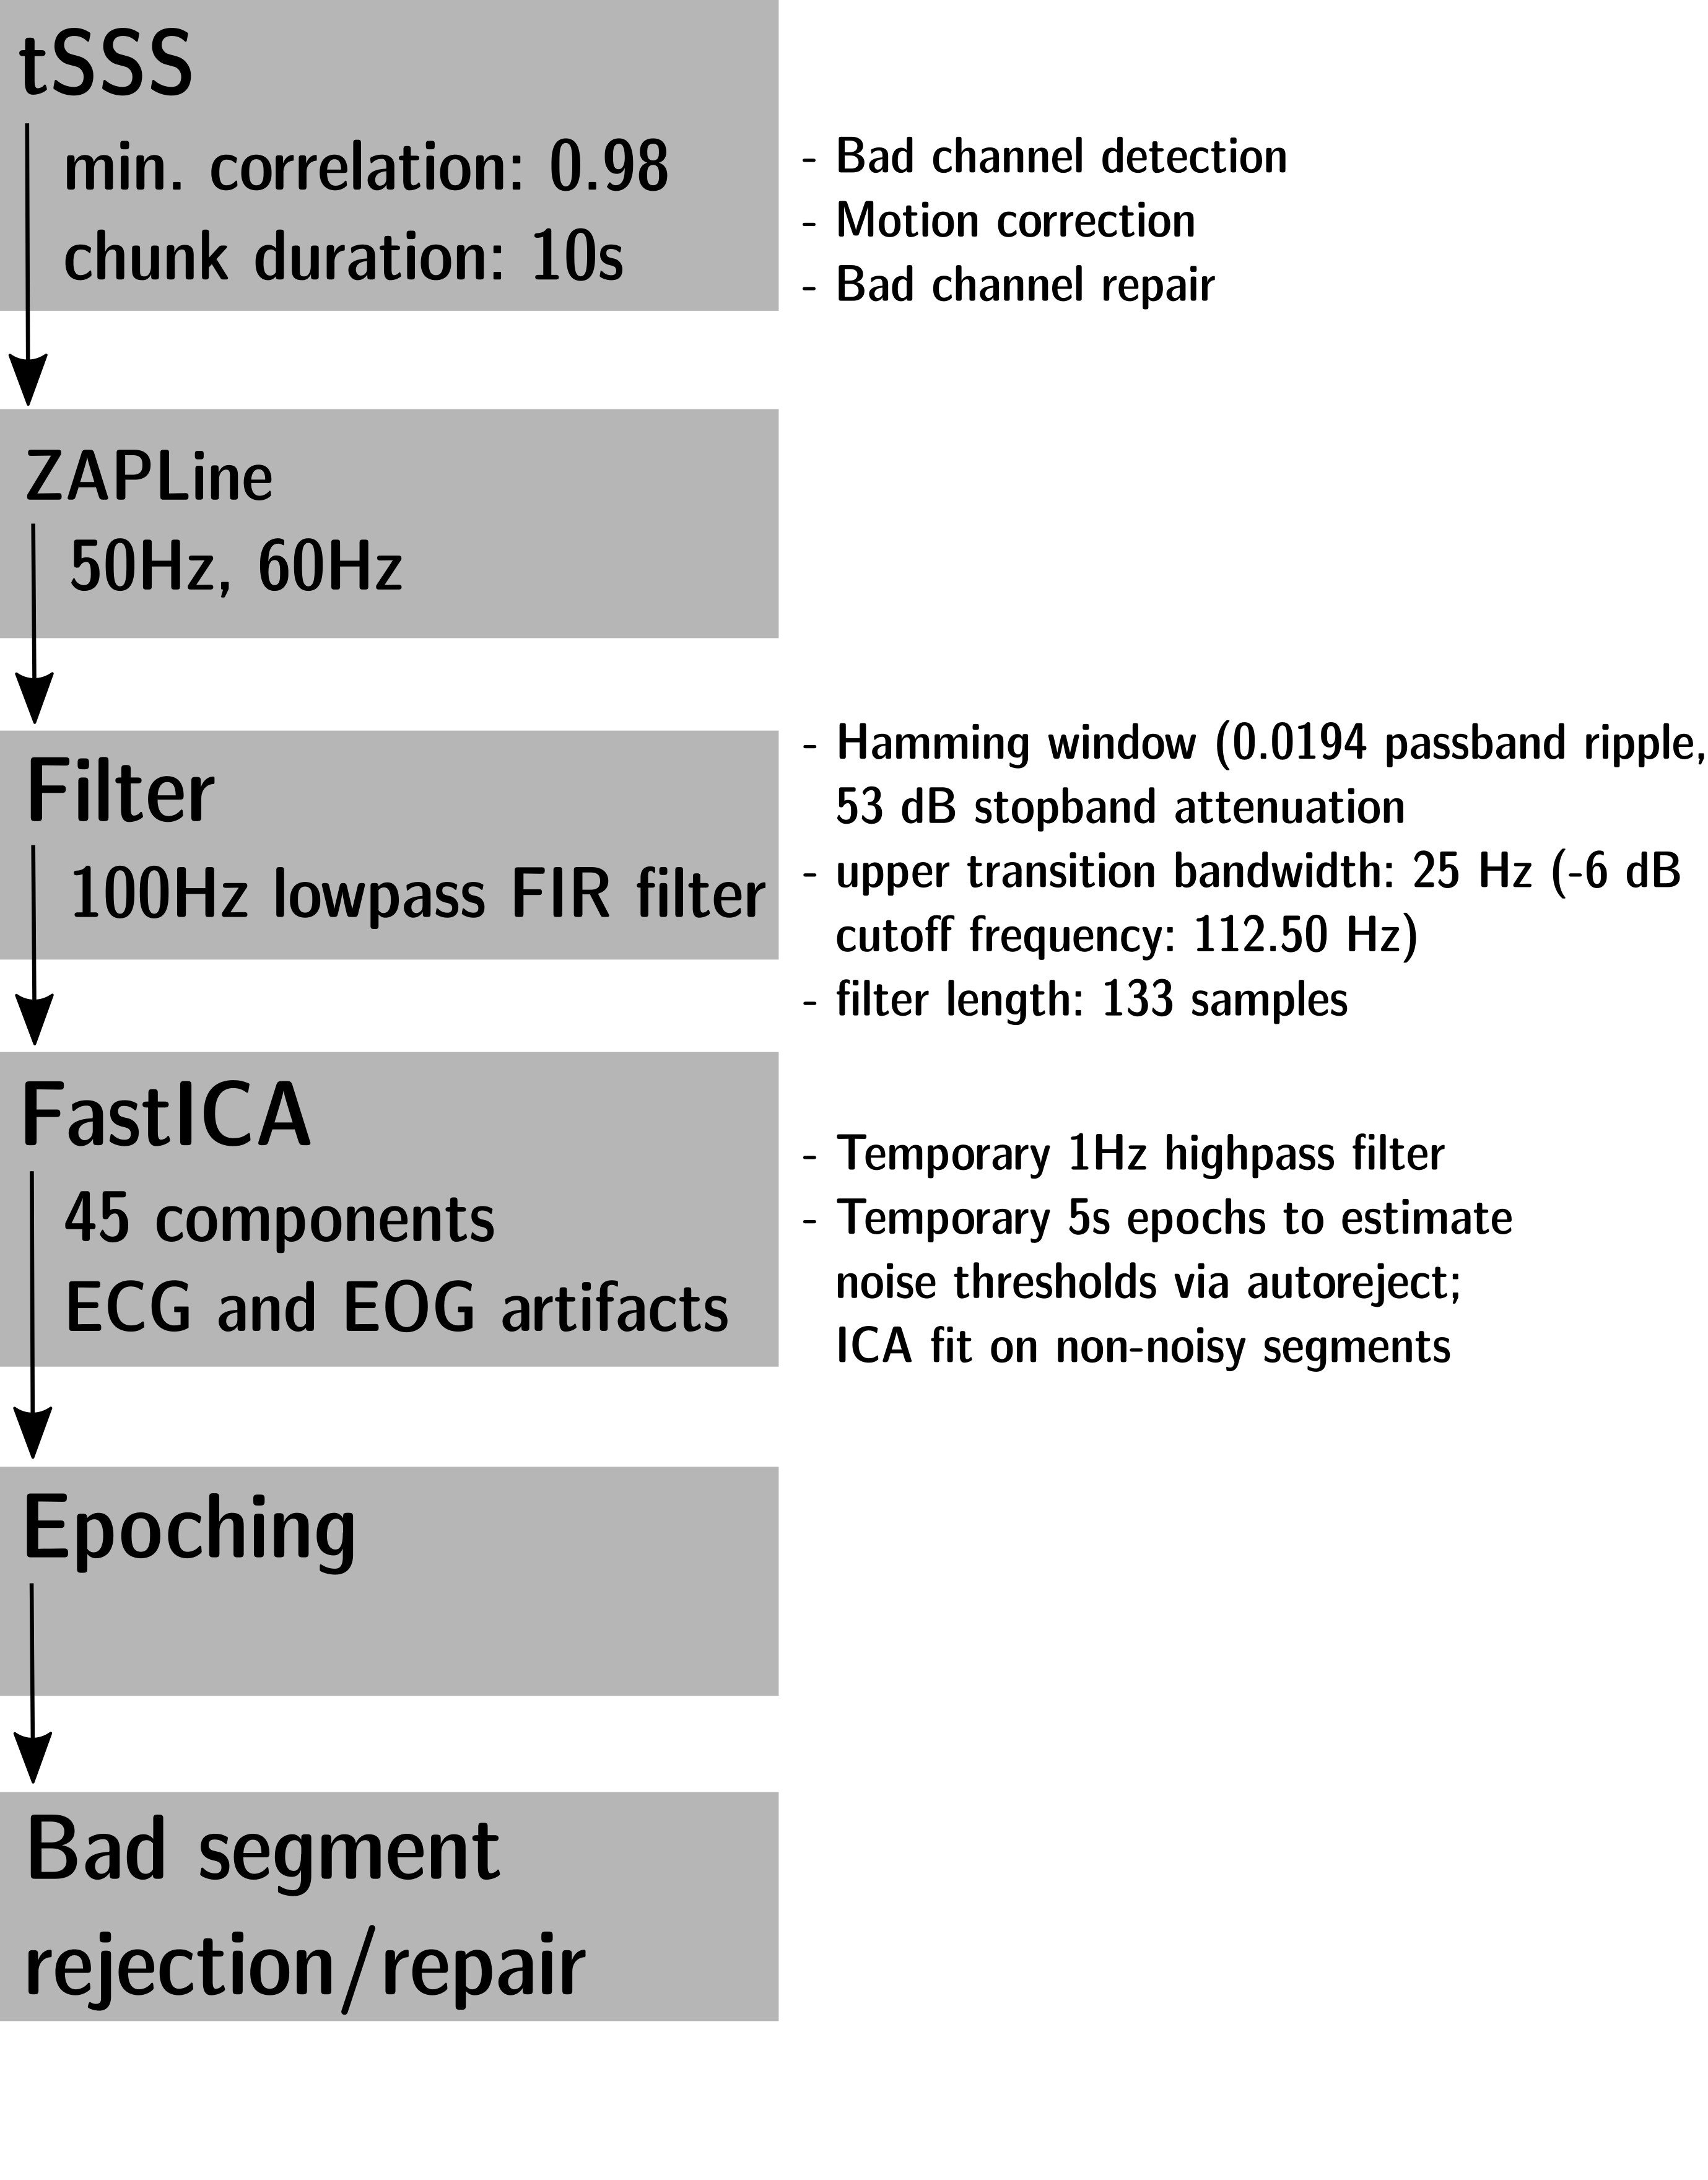
\includegraphics[width=1.\textwidth]{memento/preprocessing_overview.png}
	\caption[Preprocessing overview]{Preprocessing Overview}
	\label{fig:preproc}
\end{figure}

\textbf{Signal Space Separation} As the first step of preprocessing, the spatiotemporal extension of the \gls{SSS} method \citep{taulu2005presentation}, \textit{\gls{tSSS}} \citep{taulu2006spatiotemporal}, was applied, as is common for recordings on Neuromag MEG systems with active internal shielding.
\gls{SSS} and \gls{tSSS} remove strong interference from external noise sources and sources within the body itself from the MEG signal.
The methods can be applied on whole-scalp multichannel data when the precise sensor calibrations are known, and were initially developed as the proprietary MaxFilter\textsuperscript{TM} algorithm by Elekta Neuromag.
To this end, Neuromag systems provide a cross-talk compensation and fine calibration file which reduces interference between their co-located magnetometer and paired gradiometer sensor units and encodes site-specific information about sensor orientation and calibration, respectively.
Based on the Maxwell equations and the geometry of the sensor array, \gls{SSS} decomposes \gls{meg} signals ($\phi$) into elementary magnetic fields from sources within the sensor helmet (the \textit{internal} subspace with the signal of interest) and into an orthogonal set for fields arising from sources outside (the \textit{external} subspace with interference sources) \citep{taulu2005presentation}.
To this end, it transforms the $N=306$-dimensional signal vector into a lower-dimensional, linearly independent subspace that spans all measurable signals, the ``SSS basis'' $S$.
Its dimensionality is dependent on two user-defined truncation values $L_{in}$ and $L_{out}$, which correspond to the highest possible frequencies in the internal and external subspace.
For Elekta systems with $N=306$ channels, optimal values are $L_{in}=8$ and $L_{out}=3$ \citep{taulu2005sss}, resulting in
$n=((L_{in}+1)^2 -1) + ((L_{out}+1)^2 - 1) = 95$ dimensions (80 internal, 15 external) \citep{taulu2005presentation}.
With $n \ll N$, $\phi$ can be uniquely decomposed into internal and external subspaces $S_{in}$ and $S_{out}$, which contain the biomagnetic signal and arbitrary external interference, respectively.

%\begin{equation}
%	\begin{aligned}
%		  \phi = \sum_{l=1}^{\inf}\sum_{m=-l}^{l} \alpha_{lm} a_{lm} + \sum_{l=1}^{L_{out}}\sum_{m=-l}^{1}\beta_{lm}b_{lm}
%		\end{aligned}
%\label{eq:sss}
%\end{equation}


%\begin{equation}
%	\begin{aligned}
%		\phi &= S_x = [S_{in} S_{out}] \begin{bmatrix}
%			x_{in} \\
%			x_{out}
%		\end{bmatrix}
%	\end{aligned}
%	\label{eq:sss1}
%\end{equation}





\begin{equation}
	\begin{aligned}
			\phi &= S_x = [S_{in} S_{out}] \begin{bmatrix}
			x_{in} \\
			x_{out}
		\end{bmatrix} = \phi_{in} + \phi_{out}
	\end{aligned}
	\label{eq:sss}
\end{equation}

As the internal and external subspaces are provably linearly independent, brain signals are then reconstructed by retaining only sources inside the helmet, thus excluding external inferences.


\begin{equation}
	\begin{aligned}
    \hat{x} =
\begin{bmatrix}
	\hat{x}_{in} \\
	\hat{x}_{out}
\end{bmatrix}
= S^{\dagger}\phi \\
\hat{\phi}_{in} = S_{in}\hat{x}_{in}\\
	\end{aligned}
	\label{eq:sss2}
\end{equation}


According to \citet{taulu2006spatiotemporal}, \gls{SSS} can separate brain signals from sources >0.5m away, suppressing external interference by a factor >100.
The spatiotemporal extension \gls{tSSS} can further detect inferences from closer sources such as stimulators or pacemakers.
These are estimated based on the fact that their strength typically exceeds that of sensor noise and they thus, unlike brain signal, leak into both the internal and external part of the \gls{SSS} reconstruction.
After detecting components with a high temporal correlation between the external and internal subspaces, \gls{tSSS} removes close-by artifacts by projecting the components common to the internal and external subspace out of the internal subspace.
In the absence of nearby artifacts, \gls{tSSS} reduces to \gls{SSS} \citep{taulu2009removal}.
\gls{tSSS} was implemented using \texttt{mne-python}'s open source implementation \texttt{maxwell\_filter()} with a chunk duration of 10 seconds and a correlation threshold of at least $0.98$.
Prior to \gls{tSSS}, bad channels were detected and annotated automatically in order to prevent bad channel noise from spreading.
To compensate for head movements, measurements from the head position indicator coils were used to estimate subject motion, and motion correction was then performed as part of the \gls{tSSS} procedure: As the signal representation in the \gls{SSS} basis is device independent, internal data can simply be transformed to a sensor array corresponding to the average head position.
Similarly, formerly bad channels have also been effectively repaired by the procedure.
After \gls{tSSS}, gradiometers and magnetometers contain highly similar information and have an altered inter-channel correlation structure because they were reconstructed from a common 80-dimensional subspace \citep{garces2017choice}.


\textbf{ZAPLine filtering} After \gls{tSSS}, visual inspection revealed that minor spectral artifacts remained in the data, among them power line noise at 50Hz and a spectral peak at 60Hz, likely originating from the presentation screen's refresh rate.
ZAPline filtering \citep{de2020zapline} was performed to remove them.
Figures \ref{fig:prezap} and \ref{fig:postzap} show power spectral density plots of the signal before and after applying ZAPline filters.


\begin{figure}
	\begin{subfigure}{.49\textwidth}
		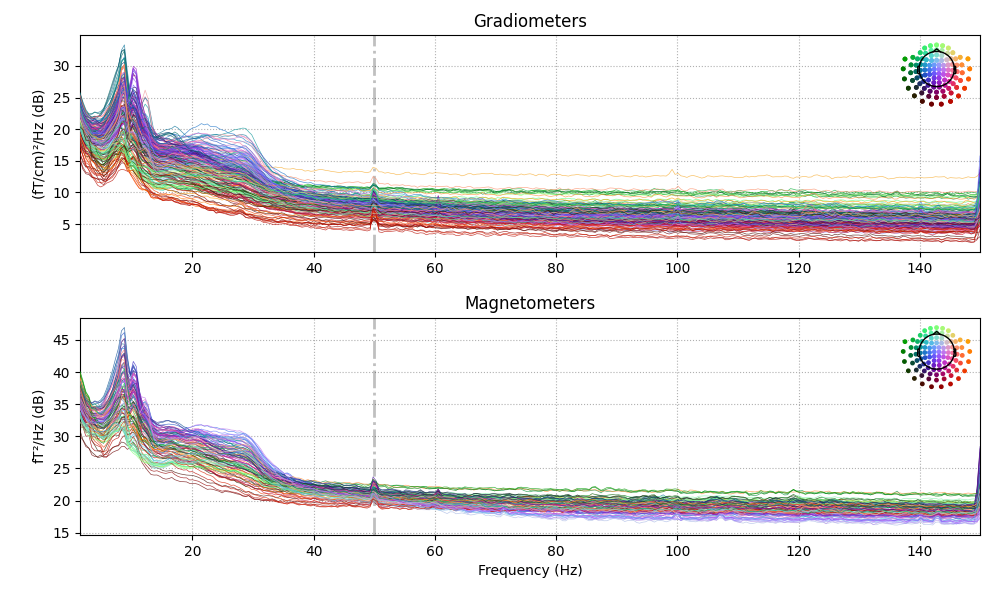
\includegraphics[width=\textwidth]{memento/psd_pre_zapline.png}
		\caption{Power spectral density before ZAPline filtering}
		\label{fig:prezap}
	\end{subfigure}
	\begin{subfigure}{.49\textwidth}
		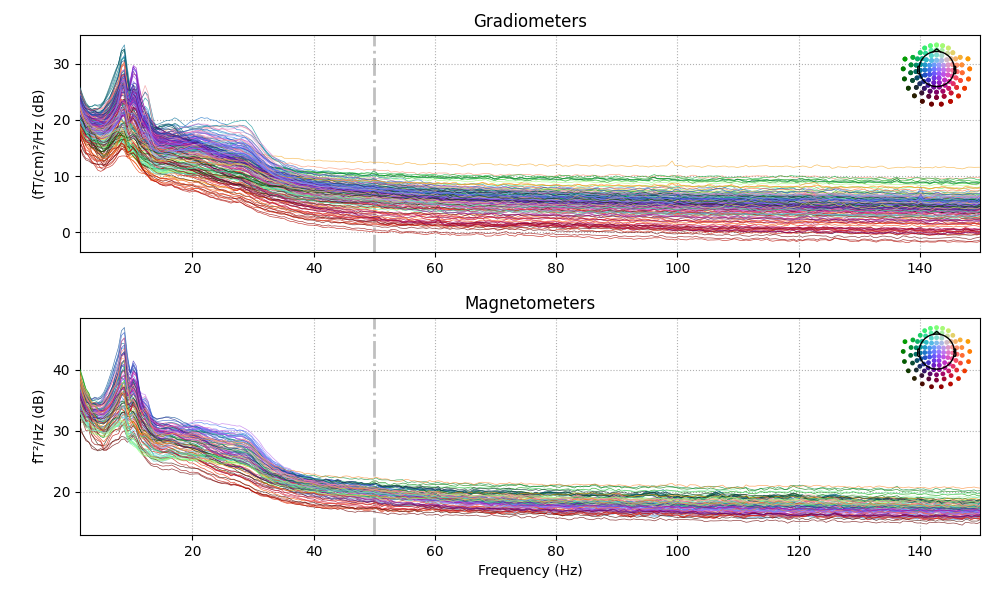
\includegraphics[width=\textwidth]{memento/psd_post_zapline.png}
		\caption{Power spectral density after ZAPline filtering}
		\label{fig:postzap}
	\end{subfigure}
	\caption[Power spectral density before and after ZAPLine filtering]{Power spectral density of all MEG channels
		from a single subject before (\ref{fig:prezap}) and after (\ref{fig:postzap}) ZAPLine filtering.
		Two spikes at 50Hz (power-line frequency) and 60Hz (likely an artifact of the stimulus presentation) are markedly reduced afterwards.
	}
	\label{fig:zapline_psd}
\end{figure}

\textbf{Filtering} Next, data were first low-pass filtered with a 100Hz lowpass FIR filter to constrain it into a frequency range of interest.
The filter properties are reported in Figure \ref{fig:preproc} and a visualization is in Figure \ref{fig:filter}.

\begin{figure}
	\centering
	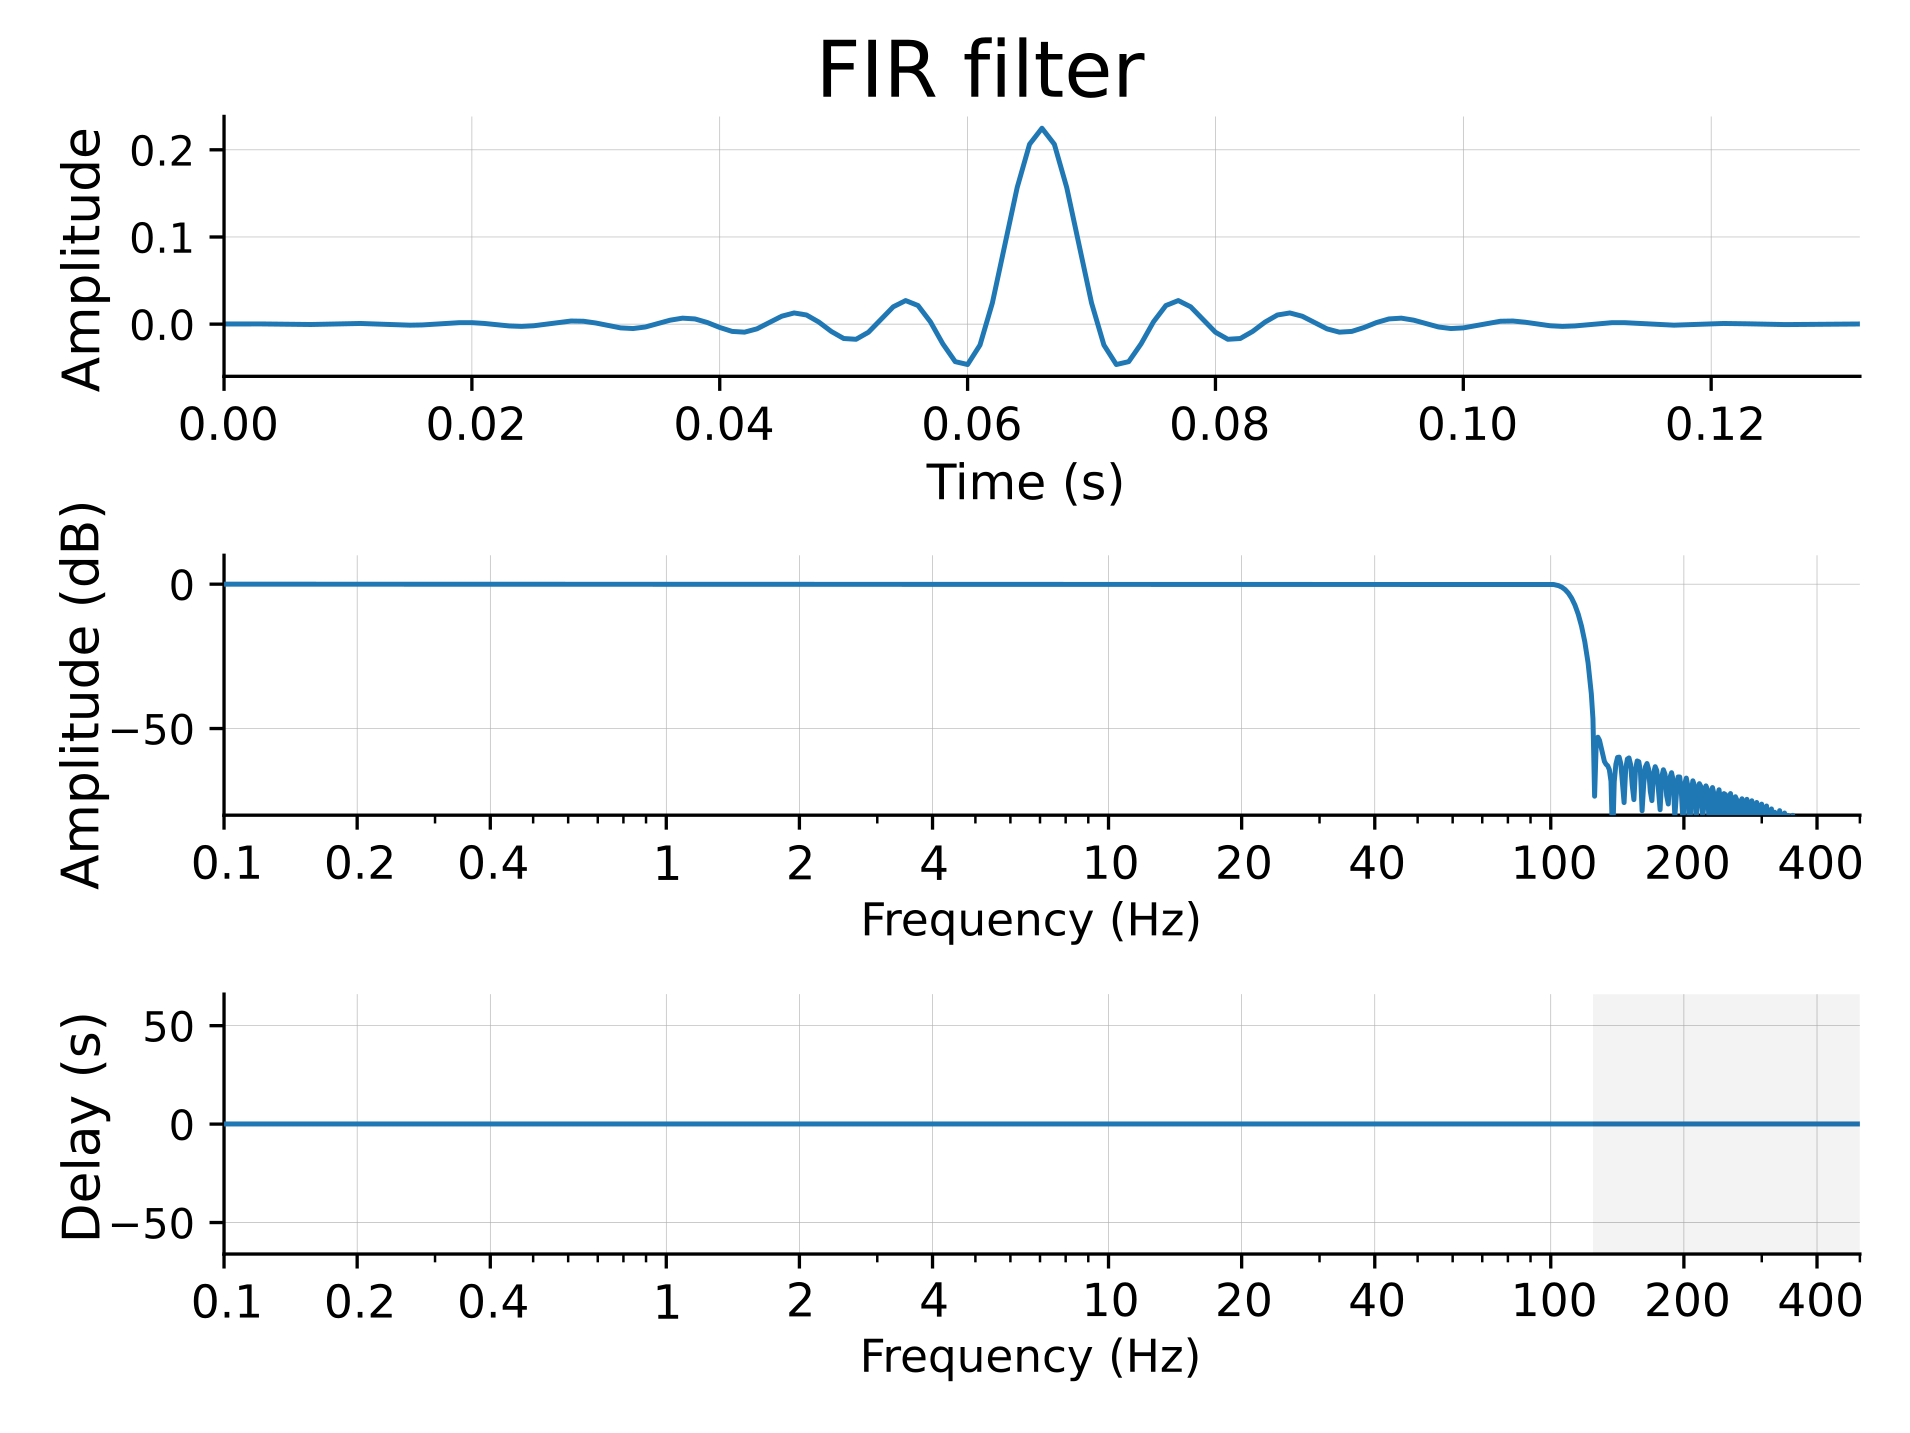
\includegraphics[width=0.4\textwidth]{memento/filter_properties_100hz.png}
	\caption[Lowpass filter properties]{Properties of the 100Hz Low-pass filter applied to the data.}
	\label{fig:filter}
\end{figure}


\textbf{Independent component analysis} As eye movements, eye blinks, heart beats, and facial muscle contractions survive \gls{tSSS}, \gls{ica} was used to detect and remove further artifacts.
% The slow drifts are problematic because they reduce the independence of the assumed-to-be-independent sources (e.g., during a slow upward drift, the neural, heartbeat, blink, and other muscular sources will all tend to have higher values), making it harder for the algorithm to find an accurate solution. A high-pass filter with 1 Hz cutoff frequency is recommended. However, because filtering is a linear operation, the ICA solution found from the filtered signal can be applied to the unfiltered signal https://ieeexplore.ieee.org/document/7319296/
As \gls{ica} is sensitive to low-frequency drifts \citep{winkler2015ICA}, the data were first processed with a temporary 1Hz highpass filter. %one-pass, zero-phase, non-causal highpass filter (firwin method, Hamming window with 0.0194 passband ripple and 53 dB stopband attenuation, a lower passband edge of 1.00, lower transition bandwidth of 1.00 Hz (-6 dB cutoff frequency: 0.50 Hz), and a filter length of 3301 samples (3.301 s)).
ICA can further be sensitive to bad segments in the recording.
Therefore, data were temporarily epoched into 5 second splits from the onset of the fixation cross.
\texttt{autoreject} \citep{jas2017autoreject}, an algorithm to reject and repair bad trials as well as to estimate bad sensors on a per-trial basis, was then used on the first 200 of these epochs to estimate the noise level and compute rejection thresholds.
Afterwards, FastICA \citep{hyvarinen1999fast} was used to decompose the signal of all epochs below these rejection thresholds into 45 independent components.
For most subjects, components corresponding to ECG activity were identified using cross-trial phase statistics \citep{dammers2008integration} with an automatically computed threshold of 0.16 for the Kuiper statistic, and \gls{eog} related components were found using Pearson correlation.
For one subject, however, the ECG channel was flat, and components were manually selected.
Afterwards, the \gls{ica} solution was applied to the continuous recording and detected ECG and \gls{eog} components were zeroed out.

\begin{figure}
	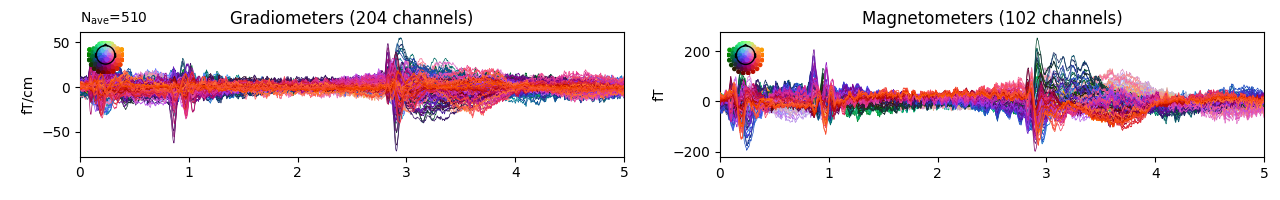
\includegraphics[width=1.\textwidth]{memento/average_epoch_cleaned.png}
	\caption[Average neural signal over the trial course]{Neural recordings from a single exemplary subject.
		Shown is the average of cleaned epochs with a length of 5 seconds from left stimulus onset, corresponding to a trial from first visual stimulation until
		1600ms after the offset of the second stimulus.}
	\label{fig:cleanepoch}
\end{figure}

\textbf{Bad segment rejection and repair} As a final step, the continous recording was chunked into epochs of varying length depending on analysis, and \texttt{autoreject} was used to detect and repair or drop bad epochs.
Figure \ref{fig:cleanepoch} shows the average of cleaned, 5 second epochs starting at the presentation of the first stimulus option for a single subject.



\section{Analysis prerequisites}
\label{decoding}

Many of the upcoming analyses are rooted in machine-learning methodology.
This section introduces relevant concepts, and summarizes common elements across analysis.
I set up the machine-learning based analyses either purely in the standard library \textit{scikit-learn} (\ref{behavioral-analysis}, behavioral analysis), using functionality from \textit{mne-python} that builds up on scikit-learn for MEEG applications (\ref{temporal-generalization-analysis}, temporal generalization analysis), or by implementing scikit-learn compatible custom estimators and scorers myself (\ref{decoding-analysis}, decoding analyses).\\
Even if upcoming analyses extend scikit-learn's capabilities, the framework's terminology remains central to describe the analysis setup in depth:
The behavioral and decoding analyses I conducted are classification problems, belonging to the family of supervised learning.
In these analyses, the goal is to predict a discrete target variable $y$ from an input data matrix $X$ with $n$ observations, for example, if a participant performs a left or right response (target) based on the stimulus properties (features) in each trial.
In scikit-learn's terms, an \textit{estimator} is what performs this prediction.
A \textit{scorer} is a method that evaluates an \textit{estimator}'s predictions on a given dataset, such as computing the accuracy from predicted and actual target labels.
A \textit{transformer} is an object that alters the input data, for example by cleaning, reducing, or expanding it, or by generating features from it.
In supervised learning, data an \textit{estimator} is trained on are labeled with the actual value of target variable $y$, but this data can not be reused to test the trained estimators' performance.
Fundamental to evaluating machine-learning applications are thus \textit{train-test} data splits.
These partition the available data into a set used to \textit{train} the \textit{estimator}, and a set yet unknown to the \textit{estimator}, used to \textit{test} how well its predictions generalize to unseen data.
The accuracy of such a model is calculated from the mismatch between predictions and actual labels in the test set, which is evaluated with a \textit{scorer}.
I set this up within a k-fold cross-validation framework, which repeats model fitting and predictions with \textit{test} and \textit{train} splits over $k$ different partitions of data such that each partition $k$ is used as a test set once.
$k$ was usually set to a value between 5 and 10 depending on the analysis.
Compared to other common forms of cross-validation in neuroimaging such as leave-one-out cross-validation, this balances the trade-off between the need for sufficient training data to reach a good fit, and the need for sufficient testing data to decrease the variance of estimated accuracy for stable estimates \citep{VAROQUAUX2017166}.
The final model evaluation is based on an average of the prediction performance in each fold, reducing the variance of the model performance estimate.
In classification problems with an unequal amount of target classes I used a stratified k-fold cross-validation paradigm, which creates splits such that the relative distribution of class labels in its split matches that in the full dataset approximately.
If testing data leaks into the training data, performance estimates get overly optimistic as the model is partially trained on the data it will be evaluated on.
To avoid this common pitfall, all machine-learning analyses were set up as a so-called \textit{pipelines}, sequences of \textit{transformers} or \textit{estimators} that chain processing steps while internally ensuring that \textit{test} and \textit{train} data are kept strictly separate.
Additionally, \textit{pipelines} ensure consistent preprocessing by applying \textit{transformers} to \textit{training} and \textit{test} data.
A \textit{transformer} common to \textit{pipelines} in all analyses was a \texttt{StandardScaler()}, transforming data to have zero mean and unit variance.
The final \textit{estimator} common to all \textit{pipelines} was a logistic regression classifier with L2 regularization and a \texttt{liblinear} solver.
This was chosen to match the choice of classifier by \citet{kaiserposter}.
%The L2 regularizer of this estimator assumes that all features are centered around zero or have variance in the same order \citep{scikit-learn-scaler}.
%Even in \gls{meg} data in which different sensor types typically have different scales, this prerequisite holds due to the combination of \gls{SSS} and scaling.
Internally, the \texttt{liblinear} solver uses a coordinate descent (CD) algorithm, which extends binary classifications problems to a multinomial case by decomposing the optimization problem into several one-vs-rest problems such that multi-target classifications become possible \citep{scikit-learn-liblinear}.\\
%Where the analysis is a decoding analysis, a model predicts a target, such as stimulus identity, based on considering the relationships between multiple \gls{meg} channels. (CONTINUE)



% From Grootswagers et al. (2017): MVPA for MEG/EEG The term “multivariate pattern analysis” (or MVPA) encompasses a diverse set of methods for analyzing neuroimaging data. The common element that unites these approaches is that they take into account the relationships between multiple variables (e.g., voxels in fMRI or channels in MEG/EEG), instead of treating them as independent and measuring relative activation strengths. The term “decoding” refers to the prediction of a model from the data (“encoding” approaches do the reverse, predicting the data from the model, reviewed in Naselaris, Kay, Nishimoto, \& Gallant, 2011; see also, e.g., Ding \& Simon, 2012, for an example of encoding models for MEG). The most common application of decoding in cognitive neu-roscience is the use of machine learning classifiers (e.g., correlation classifiers (Haxby et al., 2001) or discriminant classifiers (Carlson et al., 2003; Cox \& Savoy, 2003) to identify patterns in neuroimaging data, which correspond to the experimental task or stimulus. The most popular applications of MVPA are decoding (for recent reviews on fMRI decoding, see e.g., Haynes, 2015; Pereira et al., 2009)and, more recently, representational similarity analysis (RSA: Kriegeskorte \& Kievit, 2013).

%\subsection{machine learning concepts in scikit-learn}
%\texttt{y} is the \textit{target}, also called \texttt{outputs}, \texttt{responses}, \texttt{label} or \texttt{ground truth}.¸ Its the \texttt{dependent variable} in supervised learning, passed to an \texttt{estimator}'s fit method as y.
%\texttt{X} is the observed data. Its number of rows are the number of \texttt{samples}.
%\texttt{features} are the individual elements of a vector representing a sample. In a data matrix, features are represented as columns. Elsewhere features are also known as attributes, predictors, regressors, or independent variables.
%\texttt{samples} typically denote a single feature vector. Elsewhere, a sample is called an instance, data point, or observation. \texttt{n\_samples} indicates the number of samples in a dataset, being the number of rows in a data array \texttt{X}
%A \texttt{classifier} is a predictor with a finite set of discrete possible output values, and must implement "fit", "predict", and "score" methods, and could implement "decision\_function", "predict\_proba" and "predict\_log\_proba" methods.
%An \texttt{estimator} is an object that manages the estimation and decoding of a model. An estimators fit method takes samples X, target y, and sample properties (e.g., weights). Once fitted, the "predict\_proba" method can return probability estimates for each class from some input data X. A \texttt{score} is a method that evaluates predictions on a given dataset, returning a single
%\texttt{evaluation metrics} accept a ground truth and a prediction (e.g., output of predict, predict\_proba, etc)
%\texttt{Transformers} (or \texttt{transforms}) can clean, reduce, expand, or generate feature representation. is
%\texttt{Pipelines} sequentially chain transforms with a final estimator, and reduce the possibilities of forgetting transformations that could lead to inconsistent preprocessing applications between training and testing data and of leaking test data into training data. The purpose of a pipeline is to assemble several steps that can be cross-validated together whiule



\section{Behavioral analysis}
\label{behavioral-analysis}

As a first step, I conducted several analyses on behavioral data to check if participants' behavior matched the task demands and to inform further processing.
For the former, I conducted analyses regarding participants' performance.
One measure to evaluate performance in the experiment is the gain that participants achieved at the end of the last trial.
It is the sum of rewards accumulated over all trials, and should be higher the better participants judged stimulus values.
On average, participants gained $G=349.5$ points in the experiment (range = $[300.5, 393]$; top boxplot in Figure \ref{fig:gains}).
To assess whether this exceeds chance level performance, I conducted a simulation of $N=$~10~000 experiments with random choice behavior (bottom boxplot in Figure \ref{fig:gains}), confirming that all participants performed significantly better than chance at the 95\% confidence level (dotted line in Figure \ref{fig:gains}).
A different measure of performance is reaction time.
The average reaction time pooled across participants was $\mu_{RT}=0.93$s.
Contrary to the expectation that no-brainer trials would pose easier decisions, the difference in average reaction times for no-brainer trials compared to standard trials was negligent ( $\mu_{RTnobrainer}=0.91$s compared to  $\mu_{RTstandard}=0.94$s; Figure \ref{fig:reactiontimes}).
An inspection of average reaction times per subject revealed a small subset of slow participants with average reaction times exceeding 1.3s (Figures \ref{fig:avgreactions}, \ref{fig:avgreactionsnobrain}).

\begin{figure}[H]
	\centering
	\begin{subfigure}[t]{0.45\textwidth}
		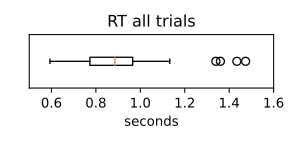
\includegraphics[width=\textwidth]{memento/behavior/average_reaction_times.png}
		\caption{Average reaction time (subject-wise)}
		\label{fig:avgreactions}
	\end{subfigure}
	\begin{subfigure}[t]{0.45\textwidth}
		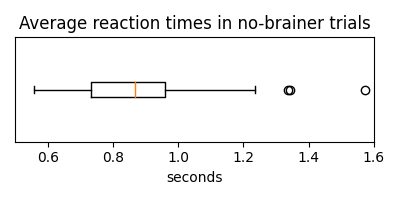
\includegraphics[width=\textwidth]{memento/behavior/average_no_brain_reaction_times.png}
		\caption{Average no-brainer reaction time (subject-wise)}
		\label{fig:avgreactionsnobrain}
	\end{subfigure}
	\begin{subfigure}[t]{0.45\textwidth}
		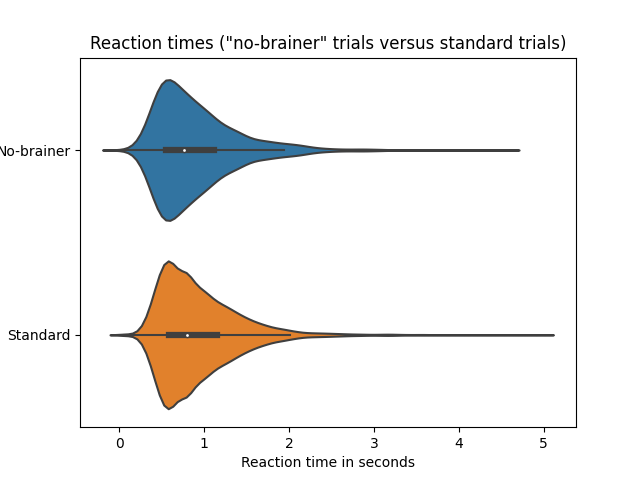
\includegraphics[trim={0 0 0 2cm},clip, width=\textwidth]{memento/behavior/memento_aggregate_reaction_times_nobrainer.png}
		\caption{Distribution of reaction times}
		\label{fig:reactiontimes}
	\end{subfigure}
	\begin{subfigure}[t]{0.45\textwidth}
		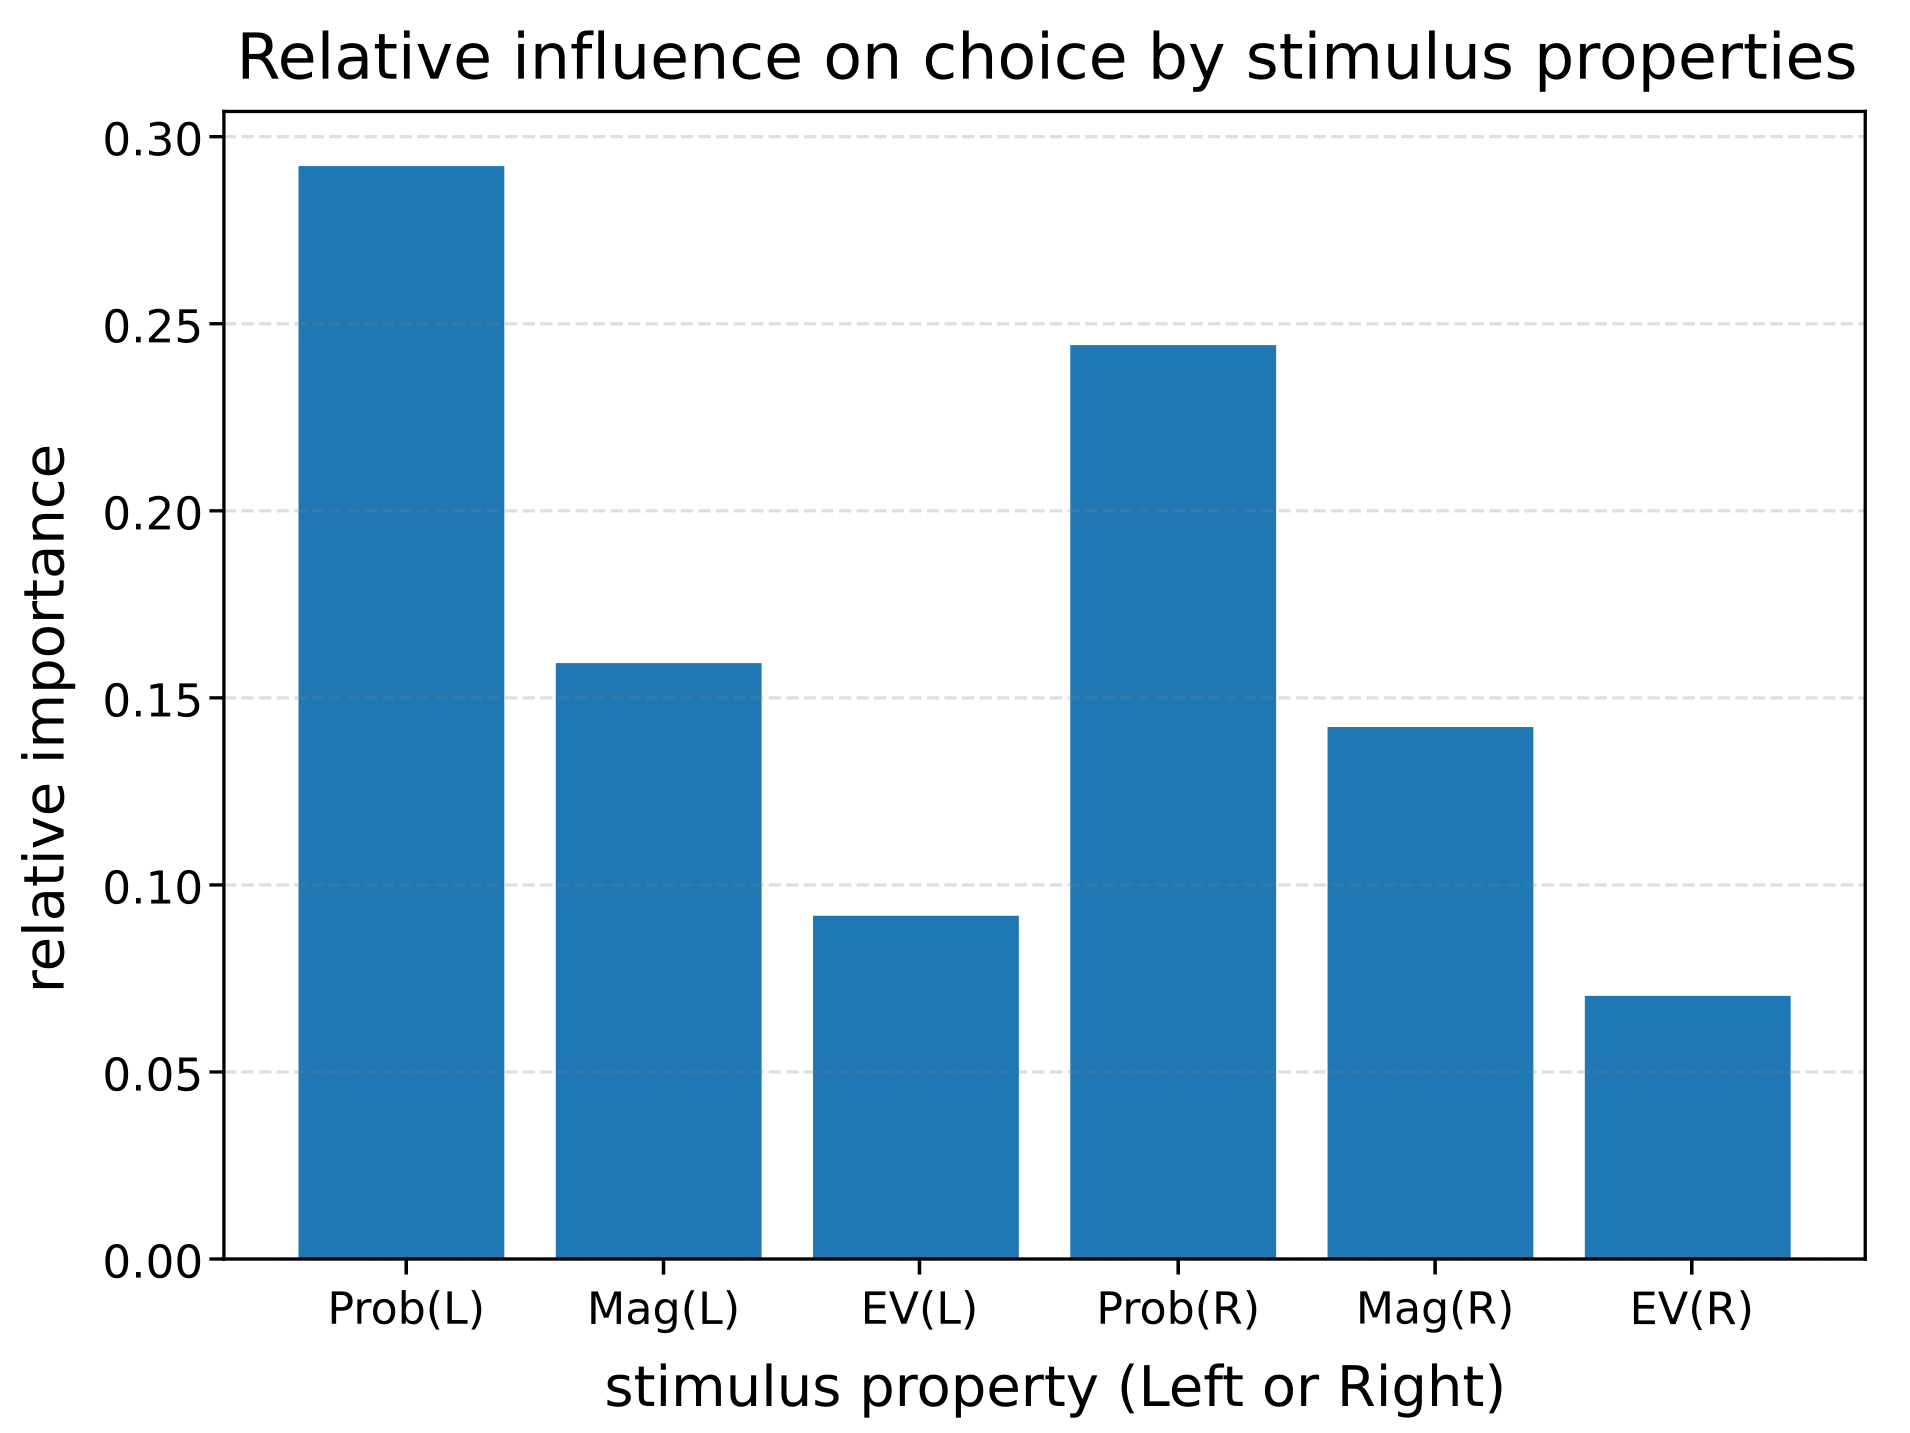
\includegraphics[trim={0 0 0 2cm},clip,width=\textwidth]{memento/behavior/average_property_importance.png}
		\caption{Parameter influence on choice}
		\label{fig:logregbehavior}
	\end{subfigure}

	\caption[Behavioral results]{Results from the behavioral analysis. a) and b) show average reaction times over trials for all subjects. c) depicts individual reaction times across trials and subjects for standard trials (orange) and trials an no-brainer trials. d) shows the relative influence of stimulus properties on choice (left option) as computed across a 10-fold cross-validated logistic regression.}
	\label{fig:behav}
\end{figure}
To inform further processing, I investigated which stimulus properties influenced participants' behavior.
The stimulus properties relevant for the eventual behavioral choice in each trial were reward magnitude (stripe frequency), reward probability (stripe orientation), and their combination (expected value).
I assessed their relative influence on choice by two means: First, by simulating different strategies by which participants could use these properties, and comparing them against the actual gains.
I created five different strategies: Pure probability- or magnitude-based strategies (choice fell on which ever stimulus had a higher value, and reduced to random choice where values were equal), primarily probability- or magnitude-based strategies (choice fell on which ever stimulus had a higher value, and in cases where values were equal, it fell on which ever stimulus had a higher value on the other property, akin to a sequential evaluation process), and an expected-value-based strategy (choice fell on the stimulus with the higher expected value, and reduced to random choice where expected values were equal).
These simulations revealed that strategies based solely on either magnitude or probability yield outcomes that are predominantly worse than participants' actual gains, bearing a single outlier.
The strategy following expected value was the best, yielding predominantly higher gains than participants' actual gains, bearing one outlier whose performance exceeded even that of 95\% of simulated experiments with the expected value strategy.
The two sequential strategies yielded a single, deterministic outcome that was close to the group average.\\
The second mean to assess which stimulus properties influenced choice was a stratified 10-fold cross-validated logistic regression analysis of left and right stimulus characteristics on choice for each subject.
The model included six predictors (magnitude and probability of the left and right option, and expected value calculated from demeaned magnitude and demeaned probability) and an intercept.
The analysis was constructed as a classification analysis following the description in Section \ref{decoding}.
Thus, the model estimated beta coefficients on a training set, and tested their predictive accuracy in a test set.
For each subject, I calculated the average accuracy over folds as a measure of model quality, and normalized beta coefficients within range $[0, 1]$ to assess their relative influence on choice behavior (Figure \ref{fig:logregbehavior}).
The average model accuracy was $0.83$ (std $=0.06$, range = $[0.68, 0.93]$).
The Spearman rank correlation between experiment performance (total gain) and model accuracy was $r=0.53$ ($p=0.012$), indicating that well-detectable influence of stimulus properties on choice was associated with higher gains in the experiment.
Across participants, reward probability had the highest relative influence on choice behavior, followed by reward magnitude, and the influence of left stimulus properties was slightly higher than that of right stimulus properties.
On the level of individual subjects this pattern held in all but one participant for whom magnitude had a higher influence than probability, and right stimulus probabilities had a higher influence than left stimulus probabilities.\\
Overall, these behavioral results confirm that participants acted according to task demands.
They further provide evidence that a majority of participants acted according to the strategy modeling decision as a sequential evaluation of probability and then magnitude (Figure \ref{fig:strategy-prob-first}).
The counter-intuitive finding that participants' reaction time was not reduced in trials that did not require integration across stimulus properties could suggests that participants did not integrate stimulus properties in any trial type, but used the same strategy in no-brainer and standard trials.


\begin{figure}[H]
	\centering
	\begin{subfigure}{0.45\textwidth}
		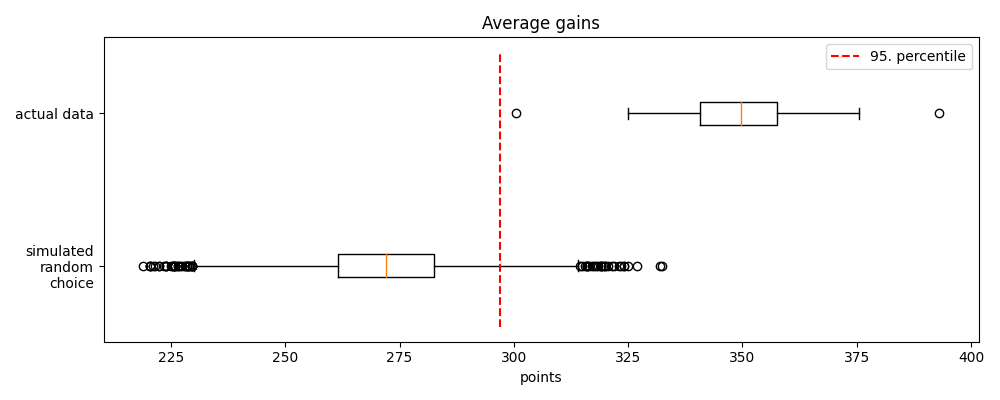
\includegraphics[width=\textwidth]{memento/behavior/average_gains.png}
		\caption{Random choice}
		\label{fig:gains}
	\end{subfigure}
	\begin{subfigure}{0.45\textwidth}
		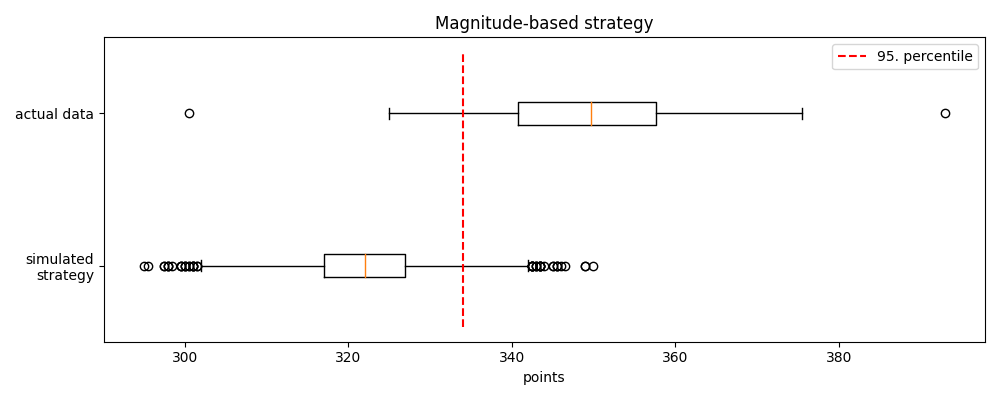
\includegraphics[width=\textwidth]{memento/behavior/gain-simulation-magnitude.png}
		\caption{Purely magnitude-based decision}
		\label{fig:strategy-prob}
	\end{subfigure}
	\begin{subfigure}{0.45\textwidth}
		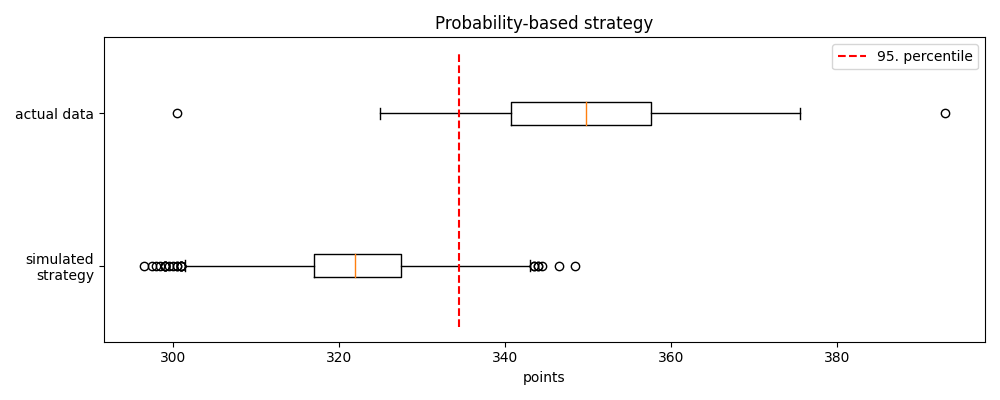
\includegraphics[width=\textwidth]{memento/behavior/gain-simulation-probability.png}
		\caption{Purely probability-based decision}
		\label{fig:strategy-mag}
	\end{subfigure}
	\begin{subfigure}{0.45\textwidth}
		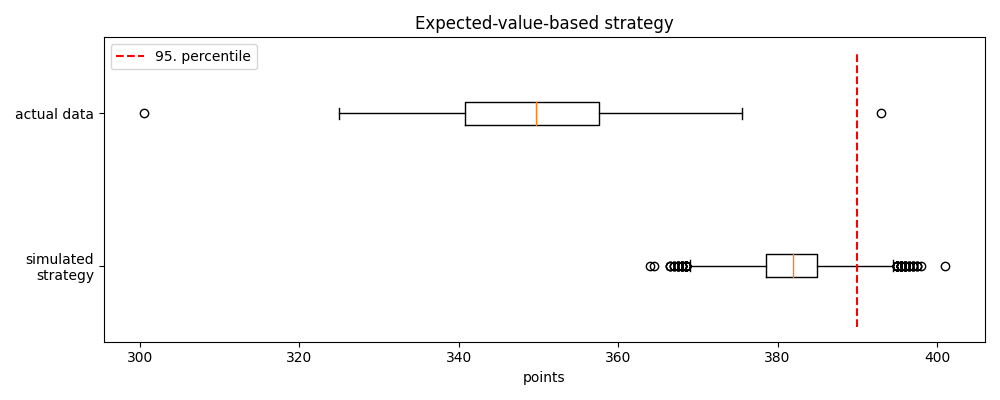
\includegraphics[width=\textwidth]{memento/behavior/gain-simulation-ev.png}
		\caption{Purely expected-value-based decision}
		\label{fig:strategy-ev}
	\end{subfigure}
	\begin{subfigure}{0.45\textwidth}
		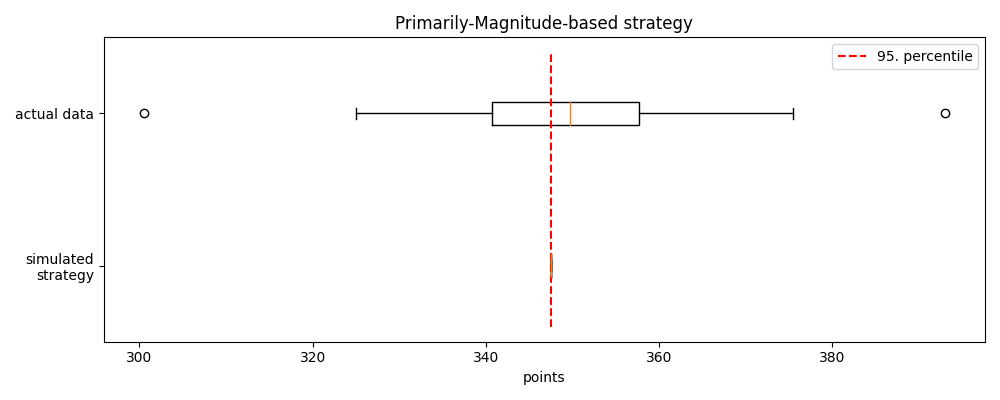
\includegraphics[width=\textwidth]{memento/behavior/gain-simulation-magnitude-first.png}
		\caption{Primarily magnitude-based decision}
		\label{fig:strategy-mag-first}
	\end{subfigure}
	\begin{subfigure}{0.45\textwidth}
		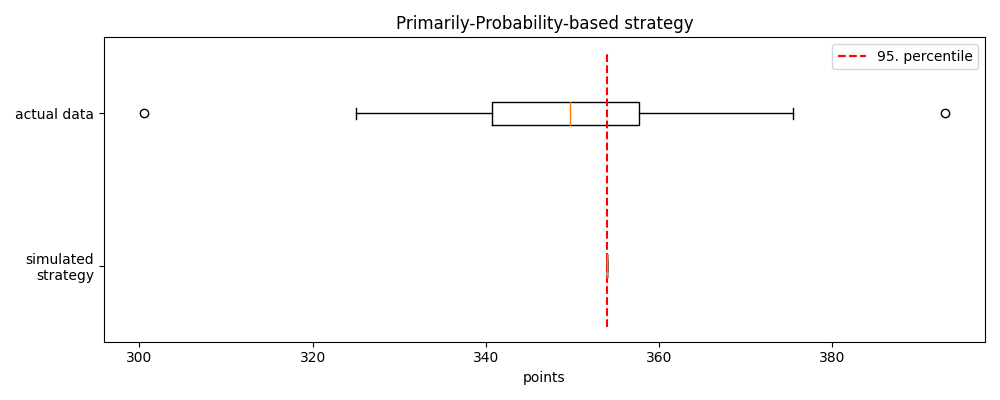
\includegraphics[width=\textwidth]{memento/behavior/gain-simulation-probability-first.png}
		\caption{Primarily probability-based decision}
		\label{fig:strategy-prob-first}
	\end{subfigure}
	\caption[Experiment gains compared to different behavioral strategies]{Experiment gains compared to different behavioral strategies. Participants' actual gains in the experiment are always plotted in the top boxplot. The bottom boxplot is a simulation of the experiment ($N=$~10~000) with different behavioral strategies. The red dotted line denotes the 95. percentile in the simulation data to allow for statistical comparisons at the 95\% confidence level. a) depicts simulated random choice behavior. Even the outlier at the bottom end of the actual results exceeds the results of more than 95\% of simulated experiments, indicating that all participants performed better than chance. b), c) and d) depict strategies that are purely based on higher magnitude, probability, or expected value, respectively, and reduce to random choice if the feature is equal across options. e) and f) depict deterministic decision strategies, based on sequentially evaluating first magnitude and then probability, or vice versa. As no random element is involved, the average gain is identical over experiment repetitions.}
\end{figure}

%\begin{figure}
%	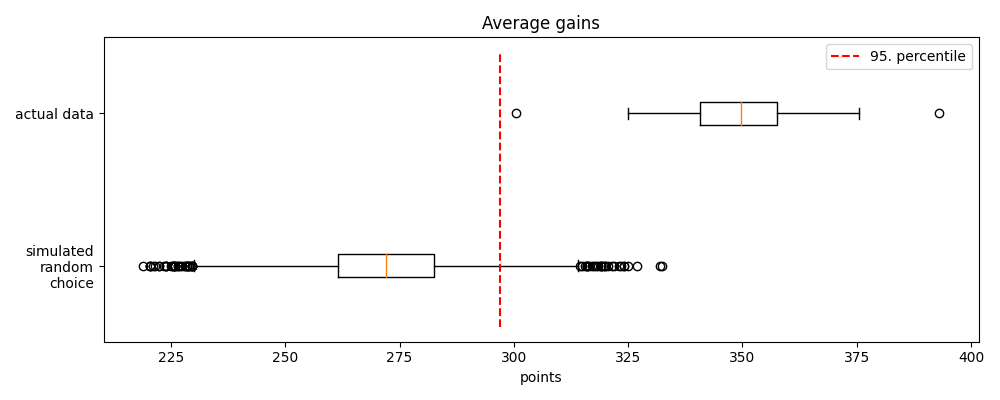
\includegraphics[width=1.\textwidth]{memento/behavior/average_gains.png}
%	\caption[Simulated versus actual experiment gains]{Participants gains in the experiment (top boxplot). The bottom boxplots is a simulation of the experiment (N=10000) with random choice behavior. Even the outlier at the bottom end of the actual results exceeds the results of more than 95\% of simulated experiments (dotted line)}
%	\label{fig:gains}
%\end{figure}


\section{Shared response modeling}

%The previous temporal generalization analysis employed a continuous decoding approach to find neural patterns and their evolution over time in the signal.
%On the group level, however, ... \\
%In typical \gls{meg} analyses, group analyses are conducted by ... .
%However, it is difficult to disentangle whether distinct neural activation patterns across individuals are due to idiosyncratic cognitive processing, or if different participants have differently encoded but shared functional states.
%In \gls{fMRI}, functional alignment methods have become popular to discover shared representations in a high-dimensional functional space \citep{haxby2020hyperalignment}.


As outlined in section \ref{preprocessing}, \gls{tSSS} decomposes the neural signal from the 306 dimensional sensor space into an 80-dimensional subspace, the \gls{SSS} basis.
The signal of interest in \gls{meg} data can thus be expressed in fewer dimensions than the $D = 306$ channels of the \gls{meg} machine.
A growing body of literature finds lower-dimensional structure in high-dimensional datasets.
In the following analyses, I therefore sought to find out whether I can find meaningful low-dimensional structure in the high-dimensional dataset by means of the \gls{SRM}.
\gls{SRM} \citep{NIPS2015_b3967a0e} is a method that combines functional alignment, a family of methods prominently established in \gls{fMRI} research to align functional topographies instead of inter-individually distinct anatomical topographies \citep{haxby2011common}, and dimensionality reduction.
A central underlying assumption of functional alignment methods can be summarized as follows: When subjects experience the same events, their brain activity patterns may differ anatomically, but they should correspond to similar cognitive processes.
\gls{SRM} was proposed as a method to functionally align the neural responses of several participants as measured with \gls{fMRI}.
For this, it models each subject $i$'s response to temporally synchronized stimuli $X_i \in \mathbb{R}^{s \times t}$ as an orthogonal subject-specific base $W_i \in \mathbb{R}^{s\times k}$ and a $k$-dimensional shared response $S \in \mathbb{R}^{k \times t}$ such that


\begin{equation}
	\begin{aligned}
		min_{w_i, s}\sum_i{\|X_i - W_iS \|}^2_F \\
		s.t. W^T_iW_i = I_k
	\end{aligned}
	\label{eq:srm}
\end{equation}

where $t$ is the number of time points, $s$ is the number of sensors, $k$ is a hyper-parameter denoting dimensionality, and $\|\cdot\|_F$ denotes the Frobenius norm.
The orthonormal constraint $W^T_iW_i = I_k$ yields the computational advantages of robustness and preserving temporal geometry \citep{NIPS2015_b3967a0e}.
Unlike, for example, \gls{pca}, the reduced dimensionality does not only emerge from the data of a single brain, but taking the activation patterns of several participants into account.
It is a latent factor model, and rather than searching for direct correspondences across subjects, an initial dimensionality reduction is used to identify latent factors that are shared across subjects and support the observed measurements.
One latent feature $k$ is a functional topography, and \gls{SRM} models the neural signal as a linear combination of subject-specific functional topographies (see Figure \ref{fig:srm-basics-multi}).\\
\gls{SRM} thus identifies common activity patterns across neural responses, and provides a method to transform the original high-dimensional signal into a lower dimensional shared latent component space.
For the \gls{meg} dataset at hand, the dimensionality is transformed as follows:
Where the original data in sensor space is a $306$ sensors $\times$ number of samples matrix, the shared response space is a $k$ features $\times$ number of samples matrix, and the subject specific weights that map between the shared space and each subject's idiosyncratic sensor space is an orthogonal matrix of dimensionality $306$ sensors $\times$ $k$ features.
All upcoming analyses used the probabilistic \gls{SRM} implementation of the \texttt{brainiak} library \citep{brainiak}.

\begin{figure}[H]
	\centering
	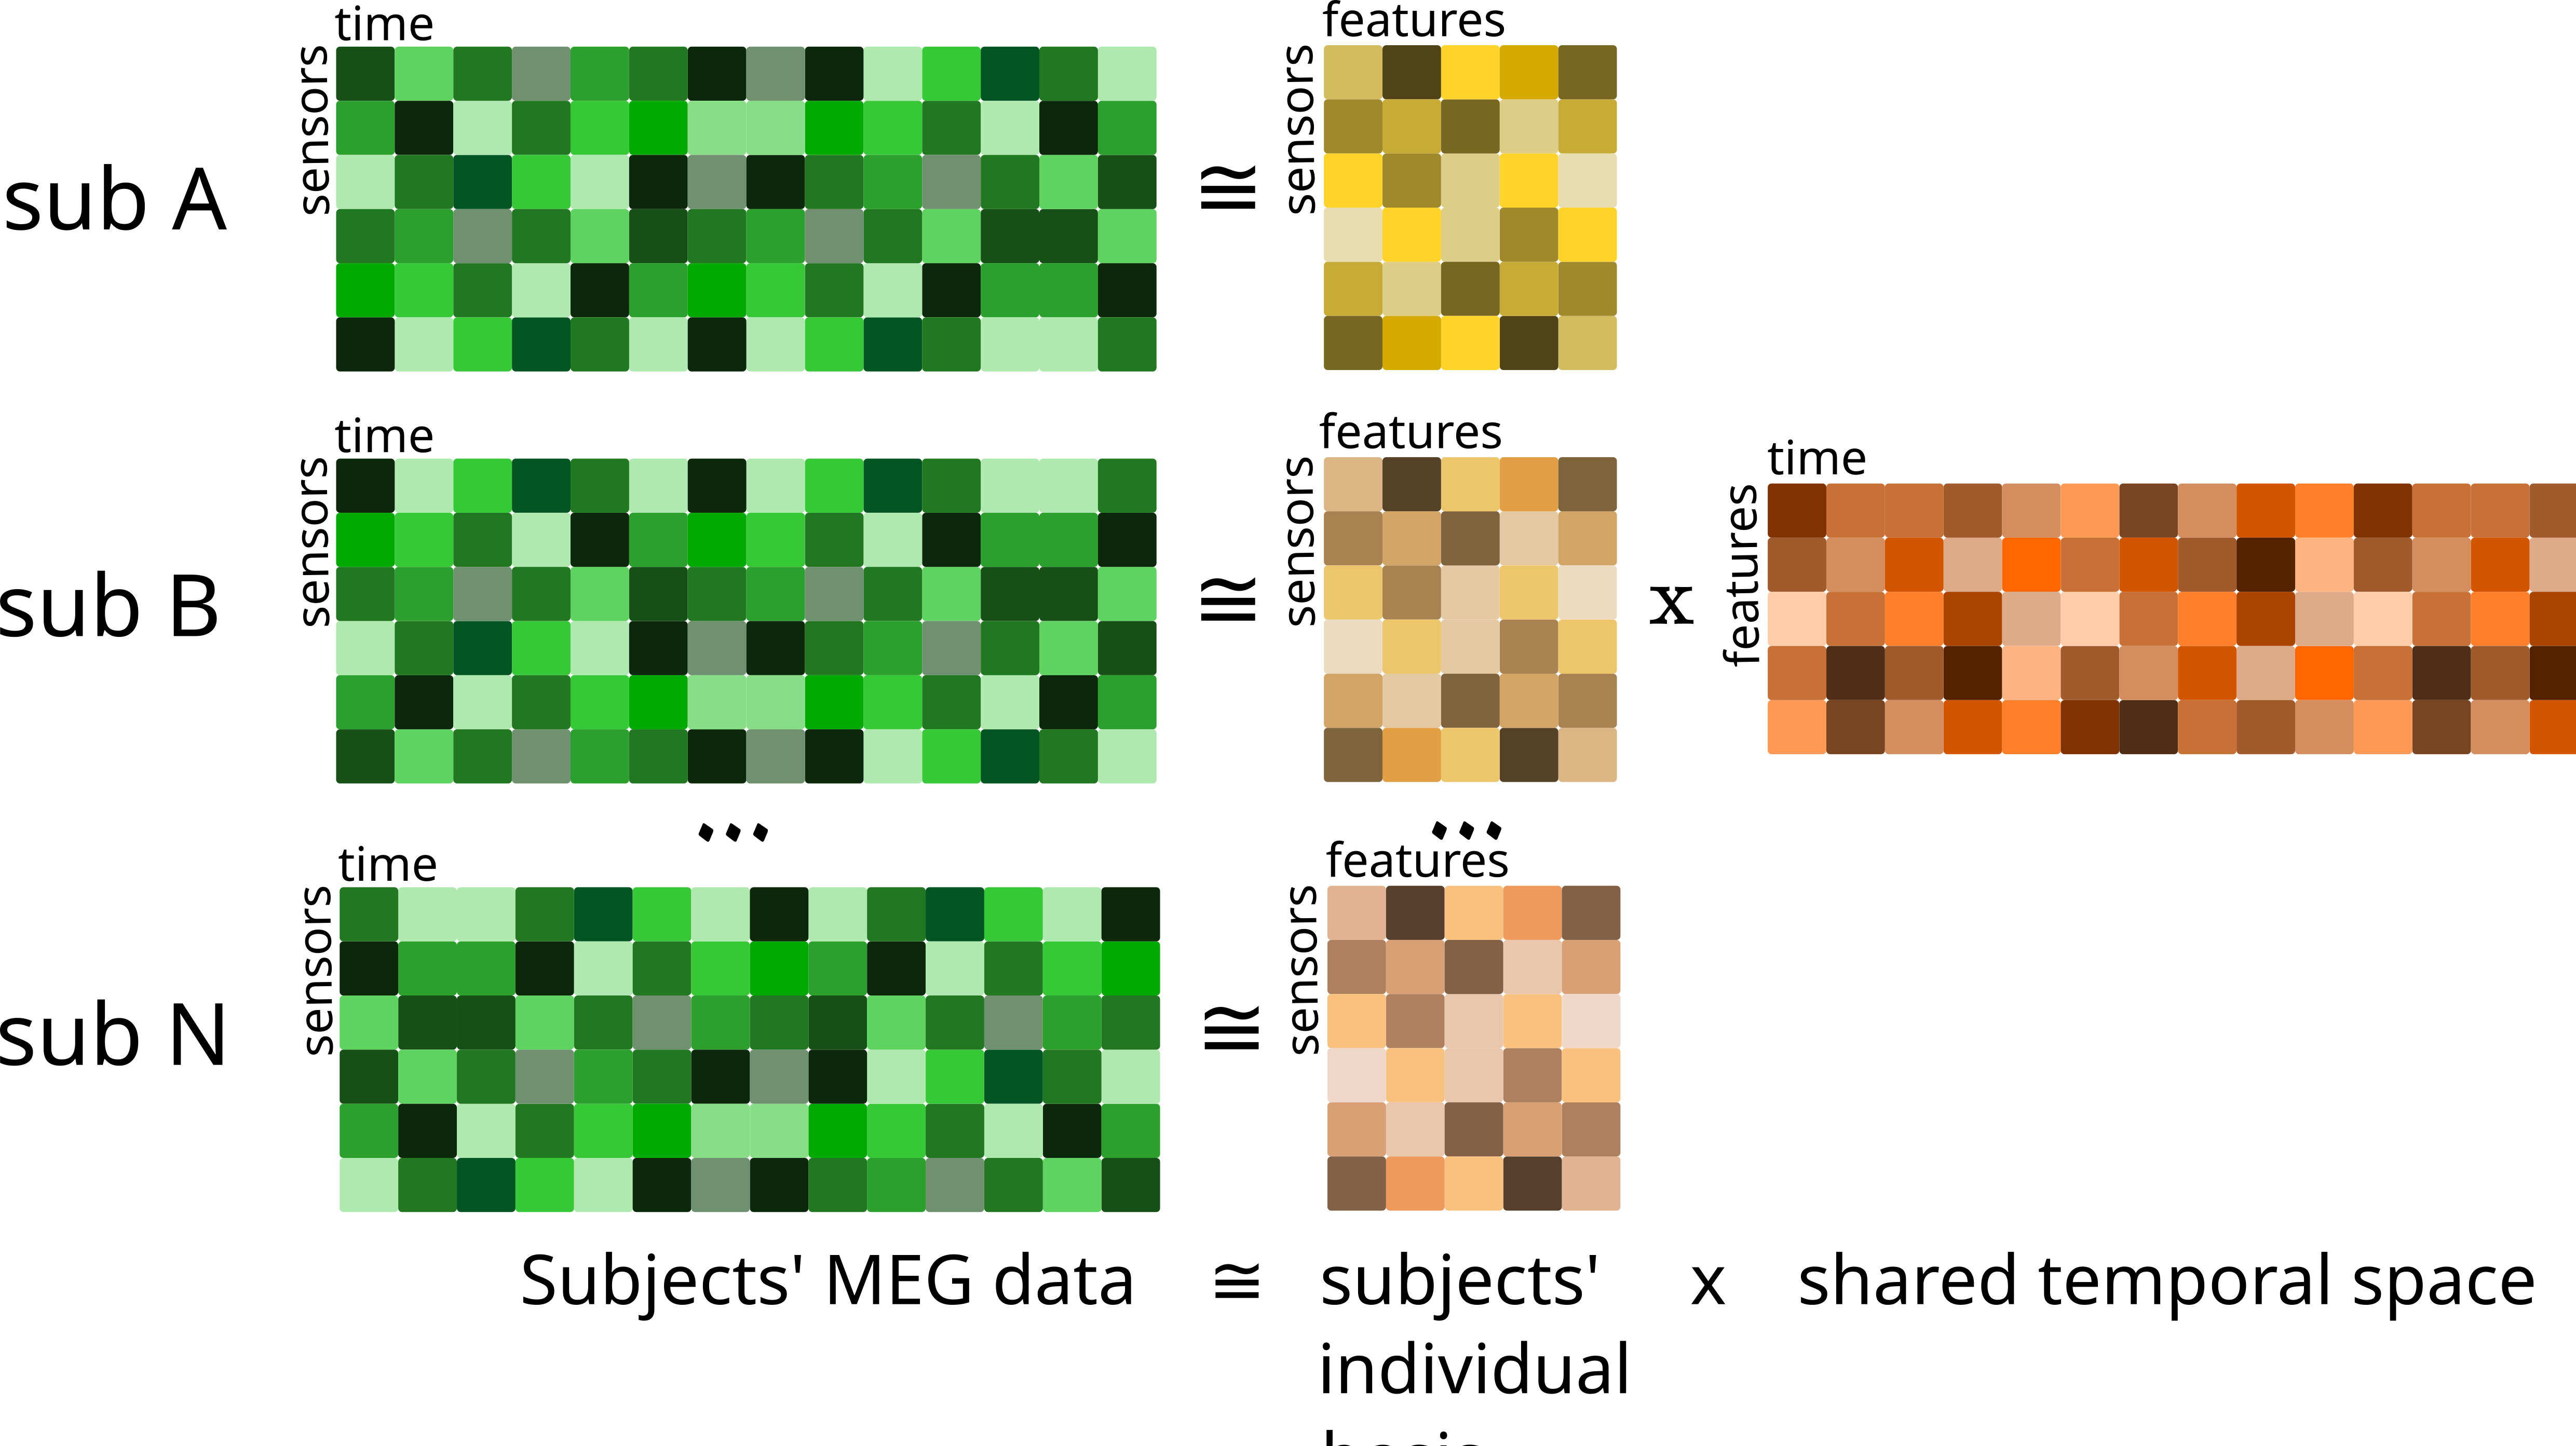
\includegraphics[width=0.7\textwidth]{memento/srm/srm_basics_3.png}
	\caption[SRM overview]{SRM overview: Sensor-by-time matrices are decomposed into a orthogonal subject specific basis matrix (sensor-by-features), a common shared feature matrix (features-by-time), and a subject-specific error.}
	\label{fig:srm-basics-multi}
\end{figure}



After an \gls{SRM} is fit, several procedures become possible.
Mapping one participant's data to a different participant's functional topography, denoising neural data by transforming the shared response via the subject-specific basis back to the individual participant's original topography, or inferring idiosyncratic signal components in individual participants' data by subtracting the shared response are applications that have been successfully demonstrated, albeit usually with \gls{fMRI} \citep{bazeille2021empirical, NIPS2015_b3967a0e, kalyani2023reduced}.
Most commonly, the \gls{fMRI} acquisitions used for \gls{SRM} and other functional alignment methods stem from feature-rich, naturalistic stimulation such as movie watching tasks \citep{haxby2020hyperalignment}.
This has the advantage that it generates a variety of cortical patterns with which these models can better generalize to unseen stimuli or novel tasks.
While the experimental paradigm at hand likely generates fewer cognitive patterns than naturalistic protocols, the fact that it is measured with \gls{meg} opens up flexible opportunities for data analysis.
One major advantage is the high temporal frequency of \gls{meg} data.
Typical recommendations of minimal acquisition lengths are in the range of 5 to 15 minutes for \gls{fMRI} data \citep{hauslerPHD} due to its long repetition time of 1-2s.
At a sampling frequency of 1kHz, \gls{meg} acquires the same amount of samples in a fraction of recording time.
The amount of samples measured in a single \gls{meg} experiment's trial can contain as many samples as an entire \gls{fMRI} experiment.
This opens up opportunities to train an \gls{SRM} based on trial time courses of a few seconds.\\ %is.
%For example, instead of investigating sharedness across different participants, an \gls{SRM} could also investigate sharedness across trials of one particular type within a single participant.

\begin{figure}[H]
	\centering
	\begin{subfigure}{.18\textwidth}
		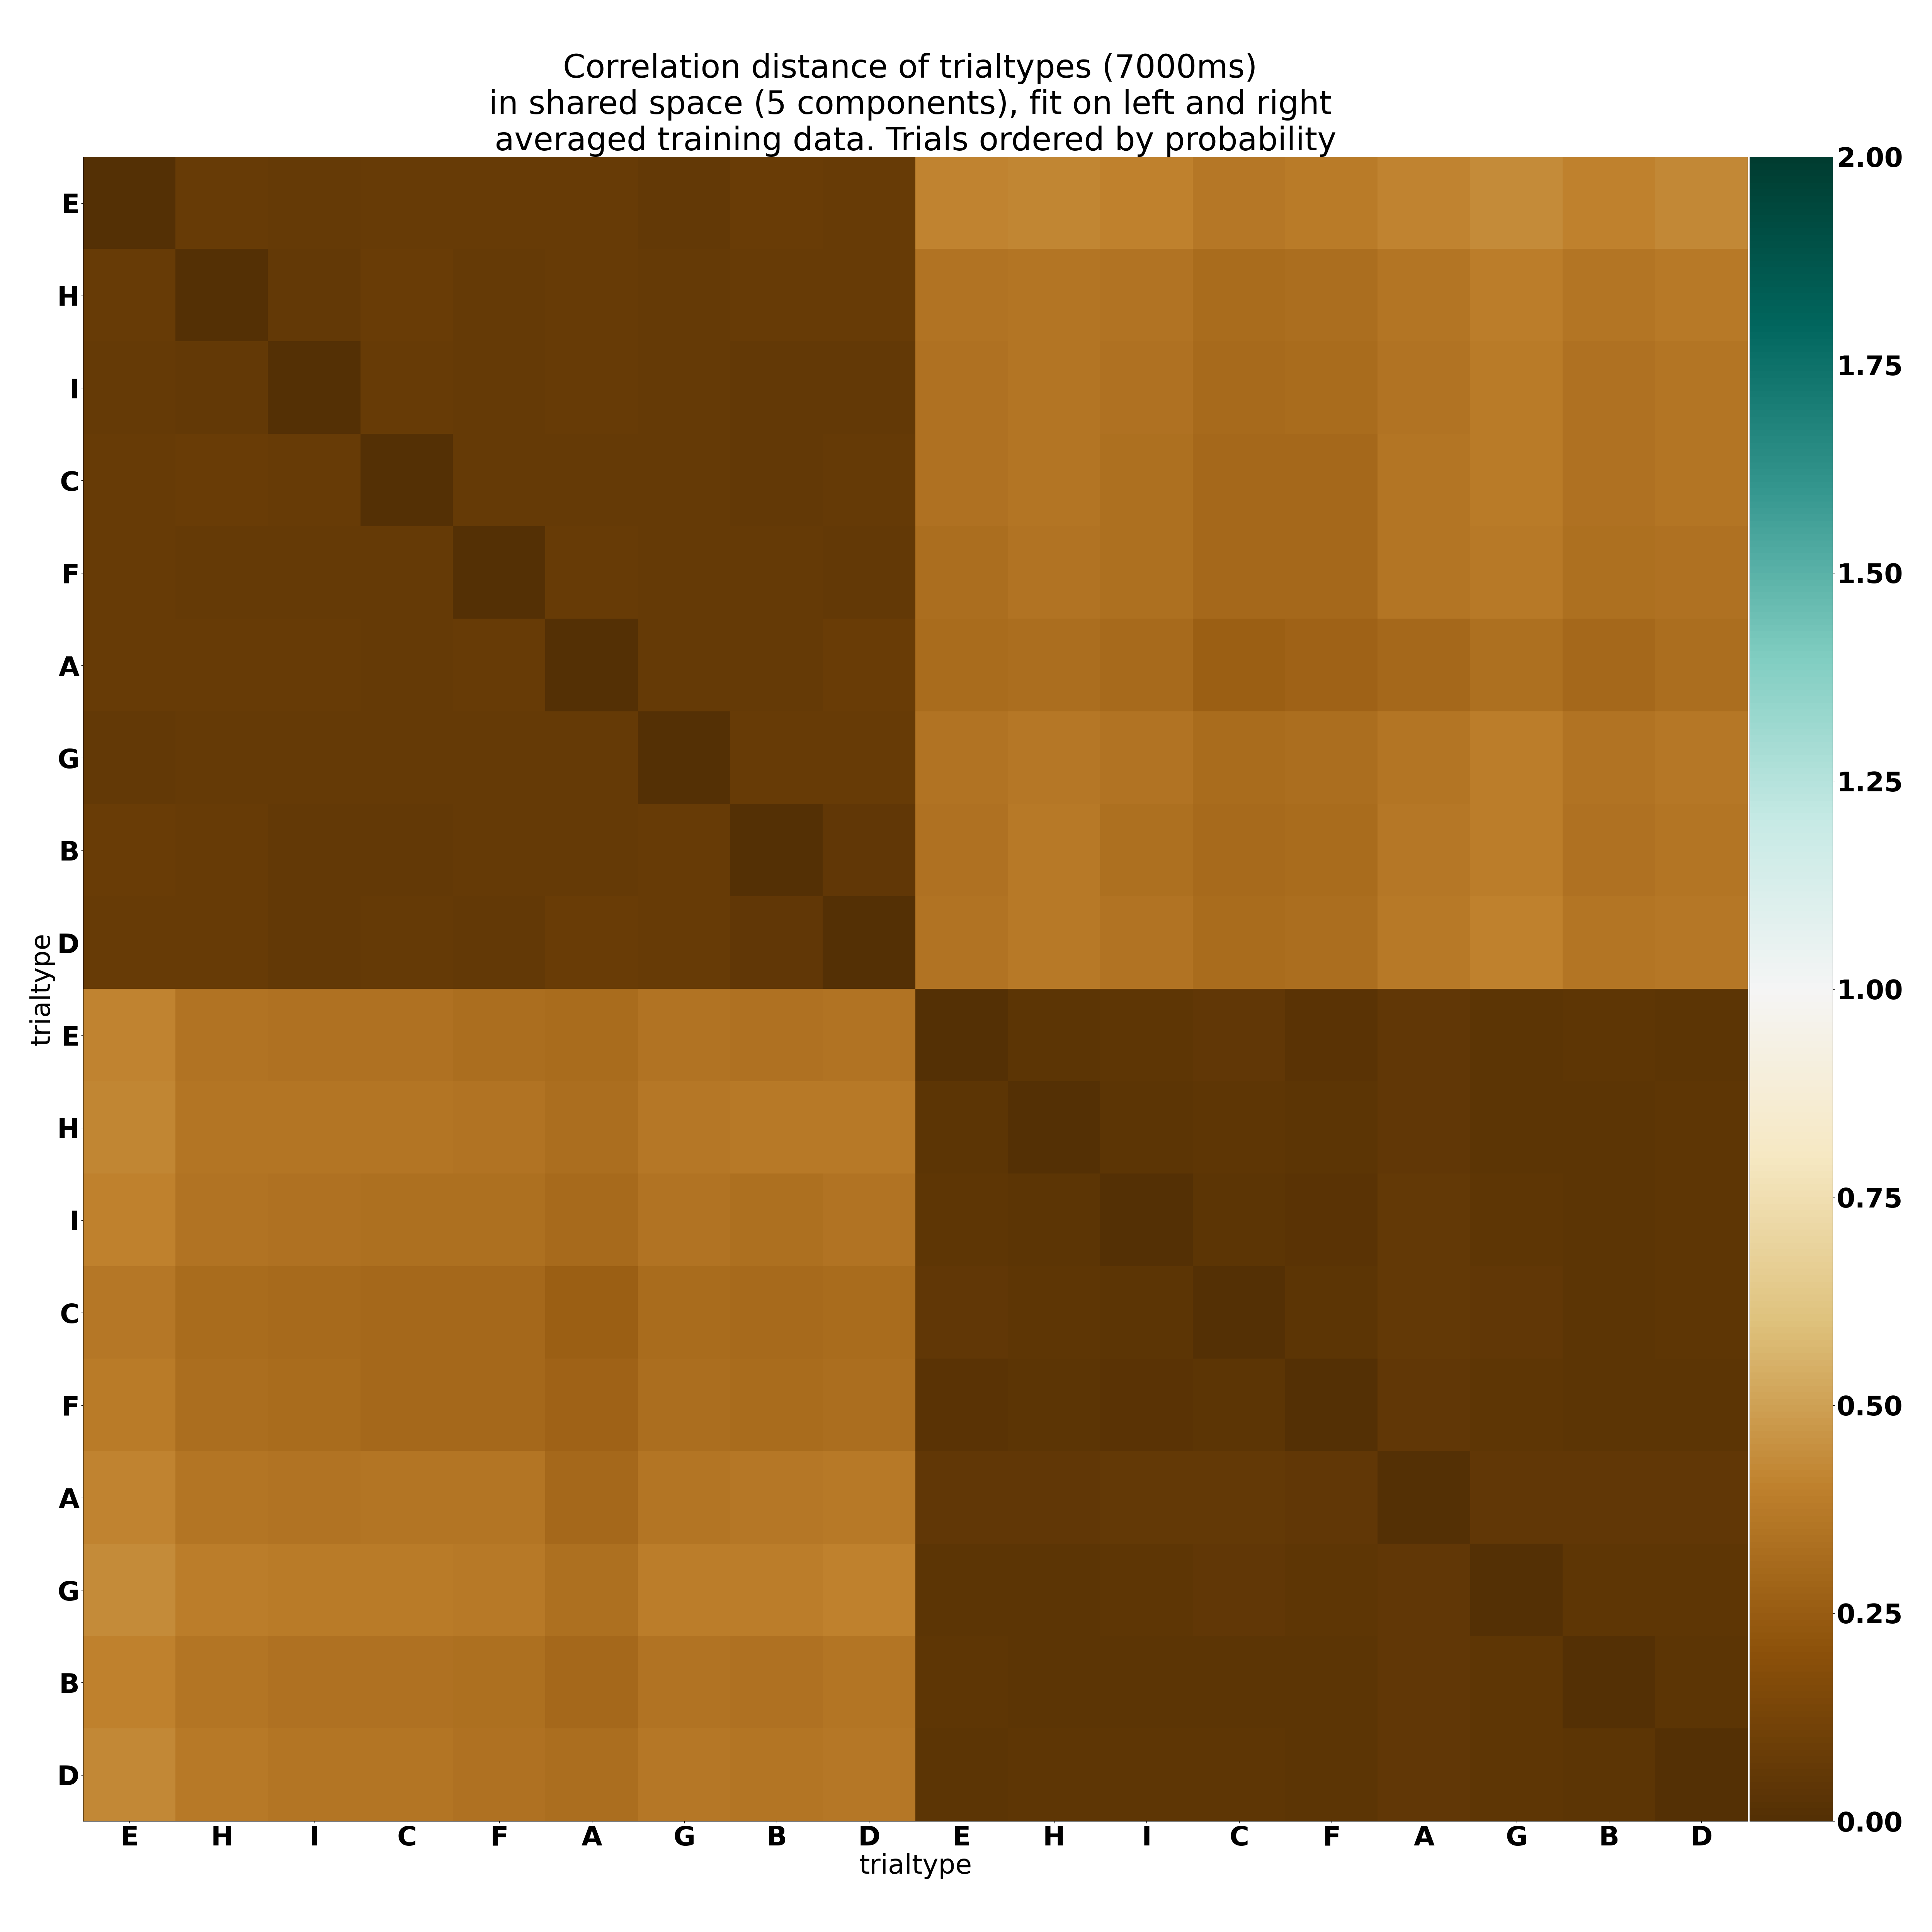
\includegraphics[clip,width=\textwidth]{memento/srm/corr-dist_avg-traindata_full-stim_5-components_order-probability.png}
		\caption{$k=5$}
		\label{fig:shared5}
	\end{subfigure}
	\begin{subfigure}{0.18\textwidth}
		\includegraphics[width=\textwidth]{memento/srm/corr-dist_avg-traindata_full-stim_10-components_order-probability.png}
		\caption{$k=10$}
		\label{fig:shared10}
	\end{subfigure}
	\begin{subfigure}{.18\textwidth}
		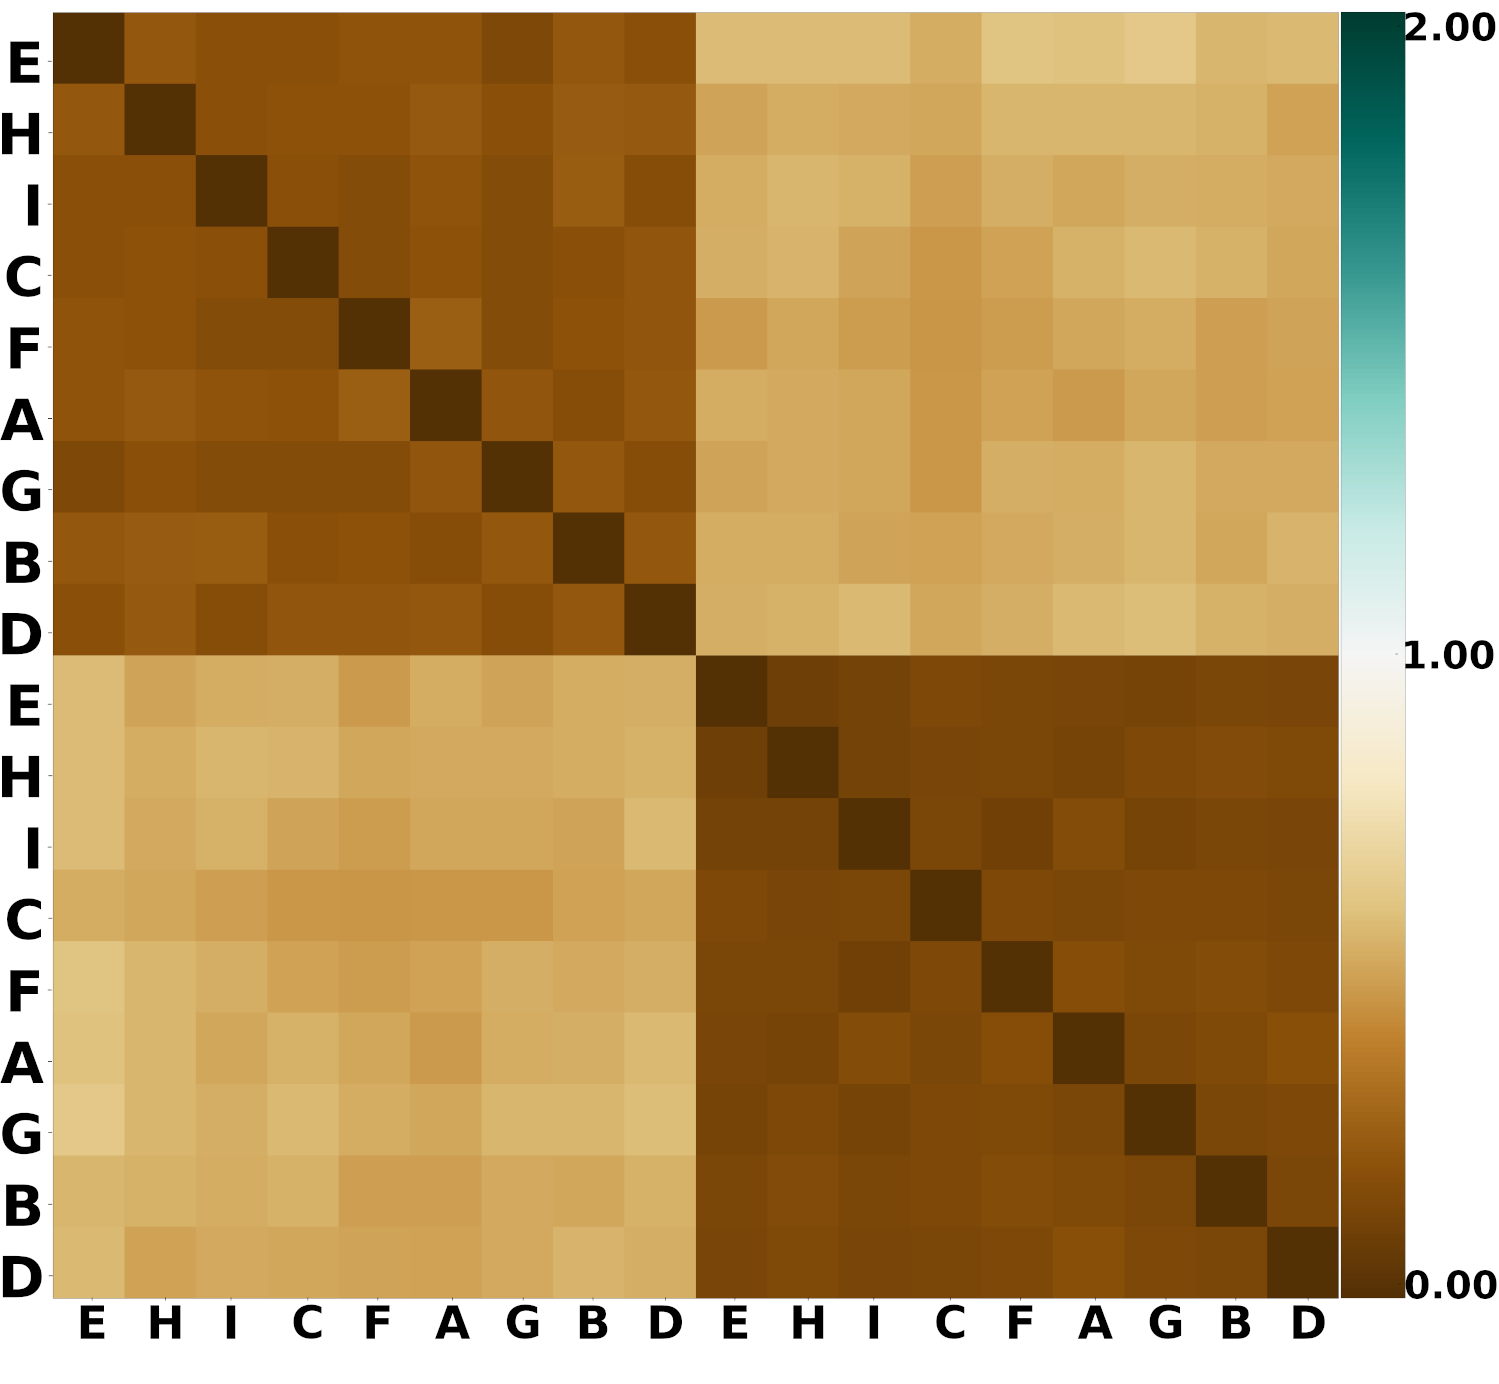
\includegraphics[width=\textwidth]{memento/srm/corr-dist_avg-traindata_full-stim_20-components_order-probability.png}
		\caption{$k=20$}
		\label{fig:shared20}
	\end{subfigure}
	\begin{subfigure}{0.18\textwidth}
		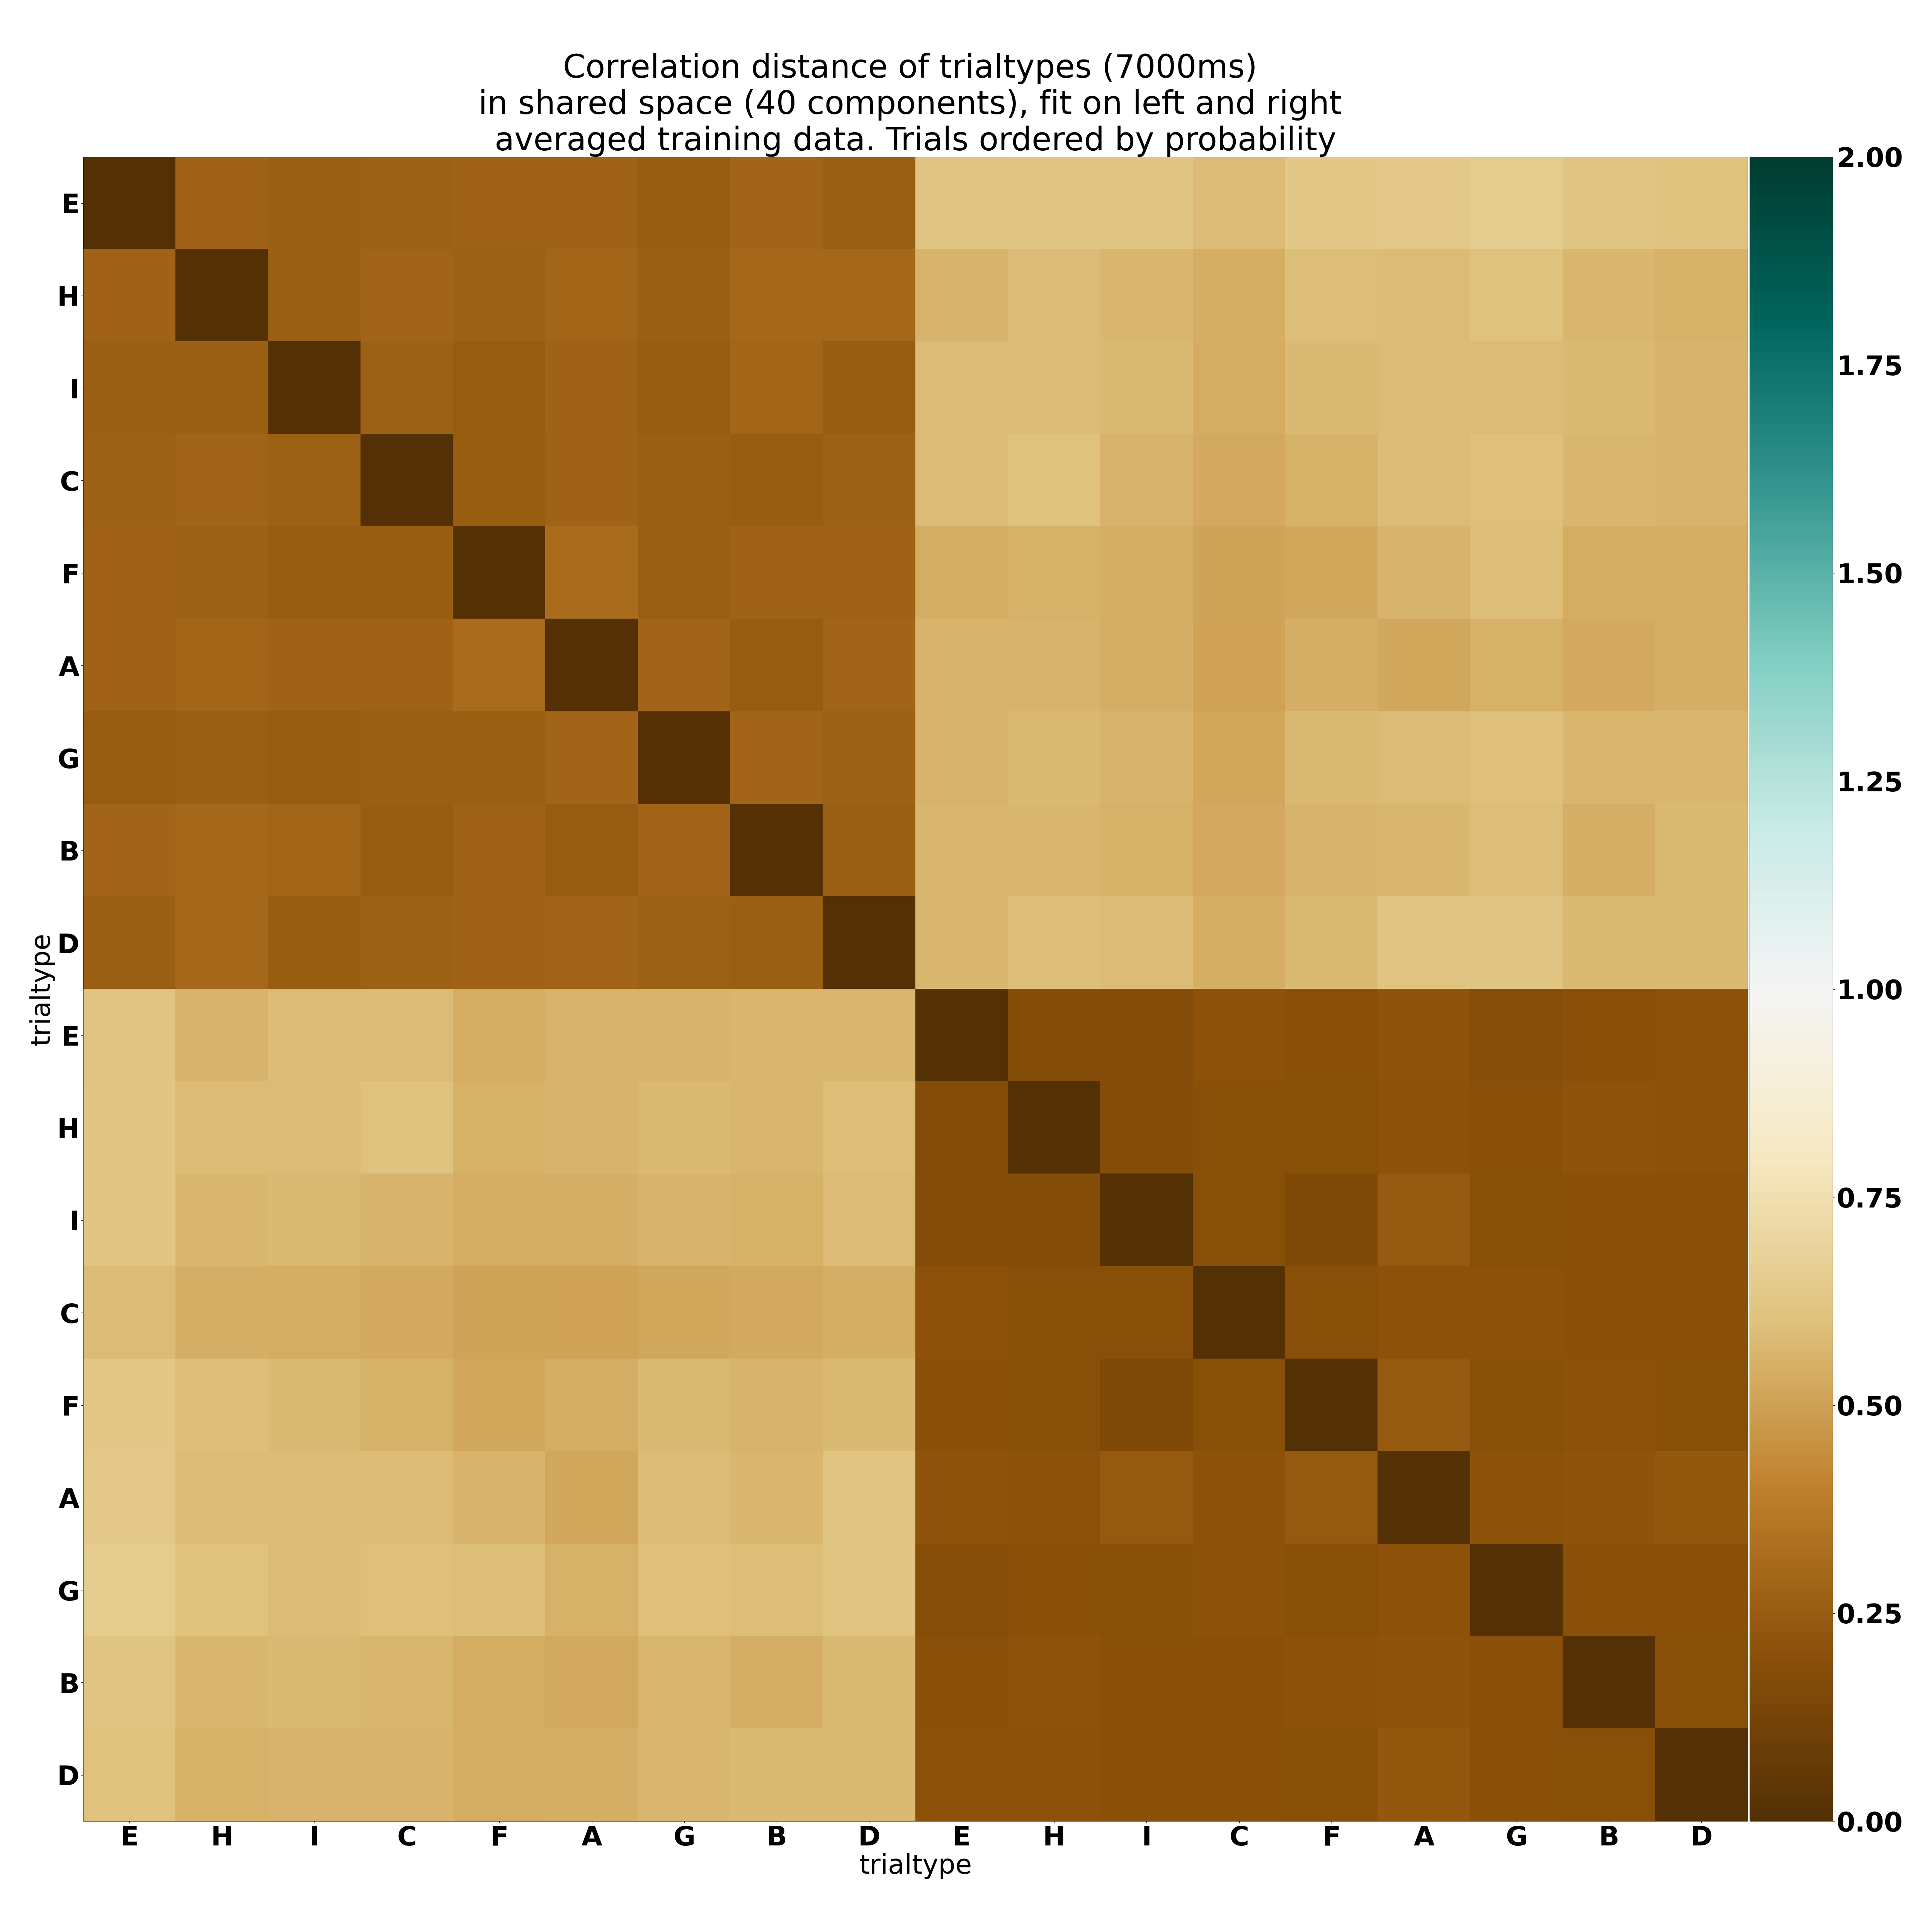
\includegraphics[width=\textwidth]{memento/srm/corr-dist_avg-traindata_full-stim_40-components_order-probability.png}
		\caption{$k=40$}
		\label{fig:shared40}
	\end{subfigure}
	\begin{subfigure}{0.18\textwidth}
		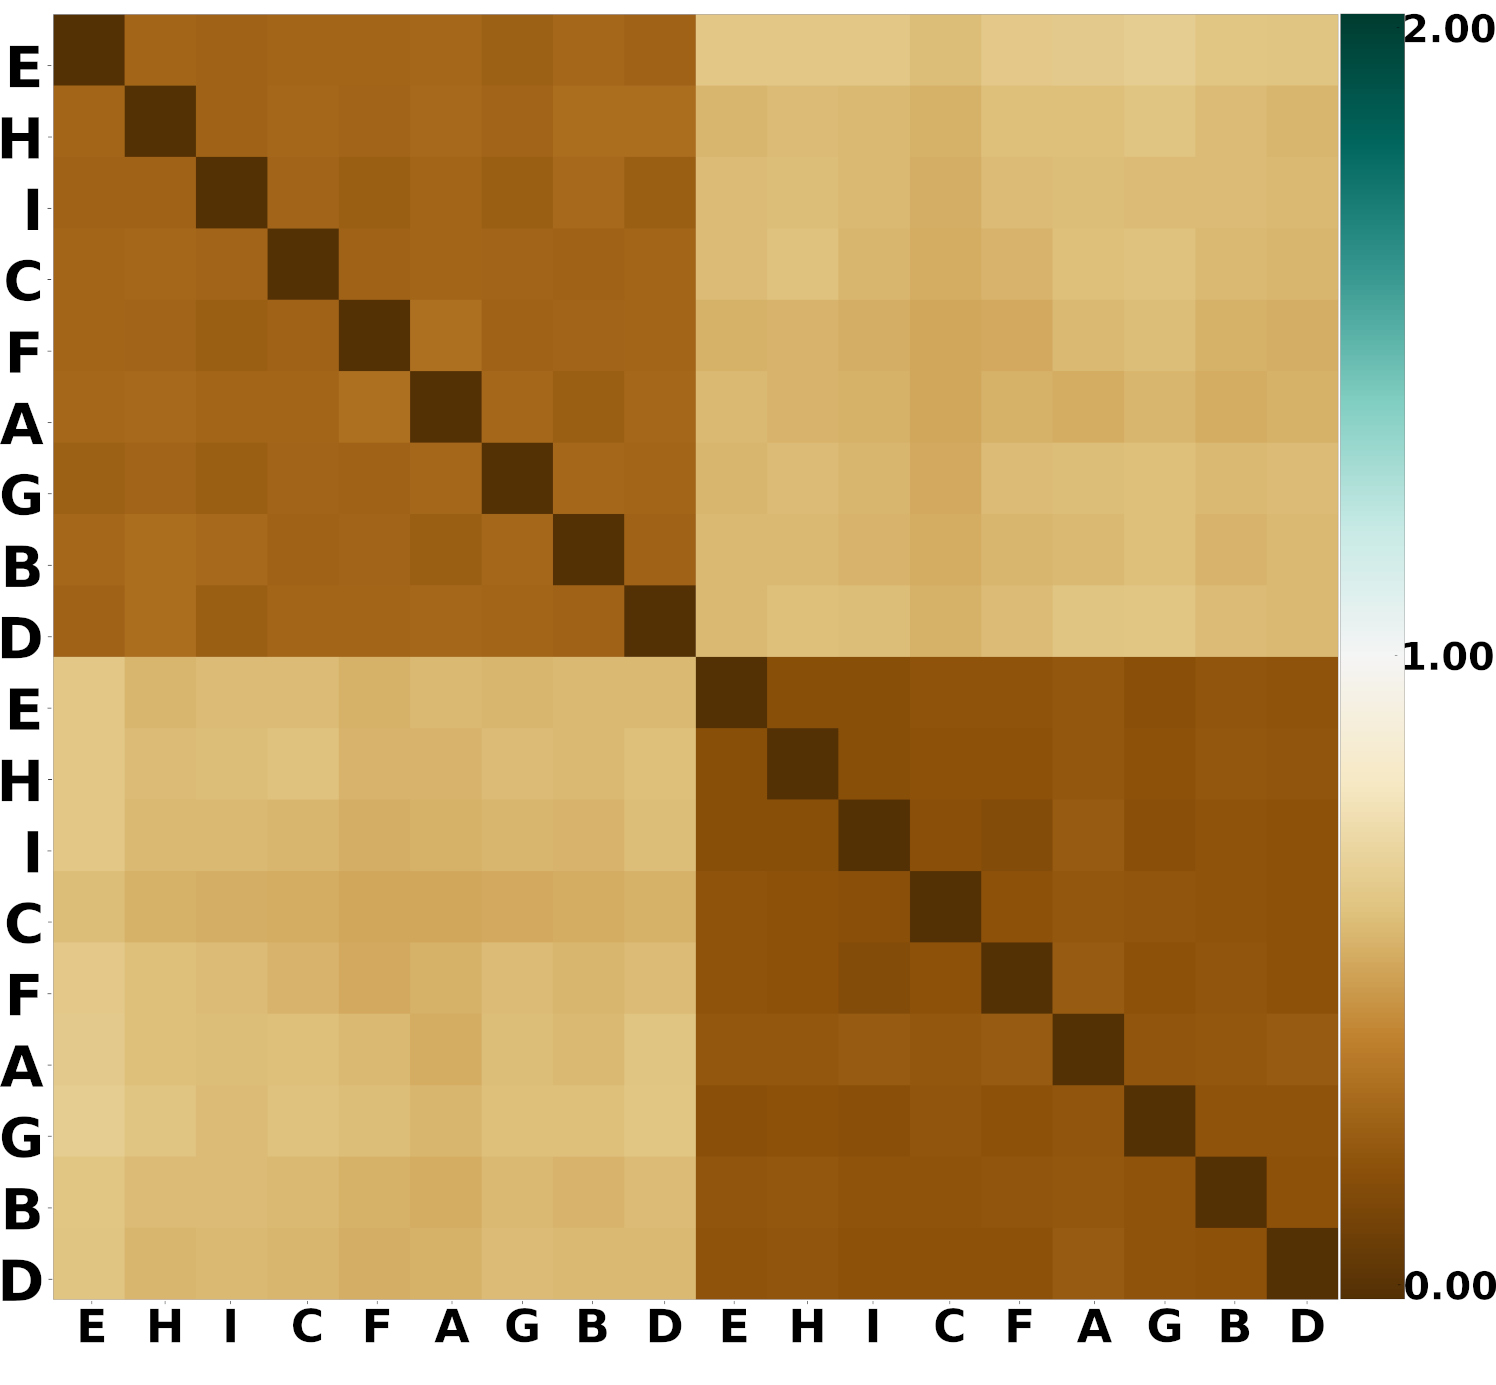
\includegraphics[width=\textwidth]{memento/srm/corr-dist_avg-traindata_full-stim_80-components_order-probability.png}
		\caption{$k=80$}
		\label{fig:shared80}
	\end{subfigure}
	%\newline
	\caption[Shared spaces of stimulus presentations]{Shared spaces of stimulus presentation, visualized as the correlation distance between the trajectories of functional topographies $k$ in the shared space between stimulus types. Darker brown values denote a stronger relationships, lighter values denote independence, and darker blue values would denote anticorrelation. Stimulus types are split into nine left and nine right options, ordered by increasing probability.}
	\label{fig:srmsharedspaces}
\end{figure}


One possible angle to analyze the experiment data with the aim of finding lower-dimensional structure is to create a shared response room with shared activity over specific parts of a trial.
A comparison of the resulting trajectories of latent components in the lower-dimensional shared space could constitute a mean to differentiate neural representations between different trial types.
Pursuing this line of thought, I conducted an analysis to investigate whether the latent functional topographies of different stimulus types differ.
Given that the nine main magnitude and probability combinations (letters A-H in Figure \ref{fig:memento_stim}) contained information to inform participants' decision process and thus should be maintained throughout the delay, I hypothesized that lower-dimensional representations might relate to these properties, for example as an abstract representation of the size of a potential reward magnitude.
To investigate this, I created training data as follows:
Within each subject, I shuffled epochs to forgo sequence effects and split them into a training and a test set, balanced with regard to the number of stimulus types, and z-scored the data within sensors for each epoch.
I then aggregated epochs in which the same stimulus was shown into average time series, separately for the left and right stimulus presentation.
Importantly, these time series were limited to the 700ms of visual presentation of the option.
This confined the shared response model to find shared functional topographies in each options visual presentation, which in turn would allow to compare the shared space of each different stimulus.
With nine common stimuli as the first and second option, respectively, this generated 18 different averaged time series per subject in training and test data.
After fitting the shared response model, I retrieved the subject-specific base matrices to transform the unseen test data into the shared space.
These spaces constitute a $k$ $\times$ 700 samples matrix, i.e., $k$ trajectories over a time span of 700ms, for each stimulus type.
To uncover differentially similar functional topographies across trial types, I then computed the correlation distance between each trial type's shared components, i.e., the similarity between the shared response during one type of trial to all other trial types, for both the left and the right stimulus option.
Correlation distance can take values in range $[0, 2]$, where $0$ indicates perfect positive correlation between vectors, $1$ indicates independence, and $2$ indicates perfect negative correlation.\\
As I had no prior assumptions about the dimensionality of the shared space, I repeated the analysis for different values of $k$.
Figure \ref{fig:srmsharedspaces} visualizes the resulting shared spaces for values of $k$ between 5 and 80.
Figure \ref{fig:srmtransformedspaces} visualizes test data transformed into this shared space across subjects.
The distance matrix is split into left and right options, which are in turn ordered by increasing probability.
The first two rows and columns in the matrix thus correspond to options with 10\% probability, the next three to options with 20\% probability, and so forth.
Instead of revealing a grouping of stimulus types by characteristics such as their probability or magnitude, however, the most marked differences lay between the sides on which the stimulus was presented.
The functional topographies in participant's neural activity were more similar for different stimuli presented on the left than the same stimulus presented on the left and right side, and the more fine-grained distances between stimulus types did not follow a pattern determined by the values of the reward magnitude or probability.


\begin{figure}
	\centering
	\begin{subfigure}{.18\textwidth}
		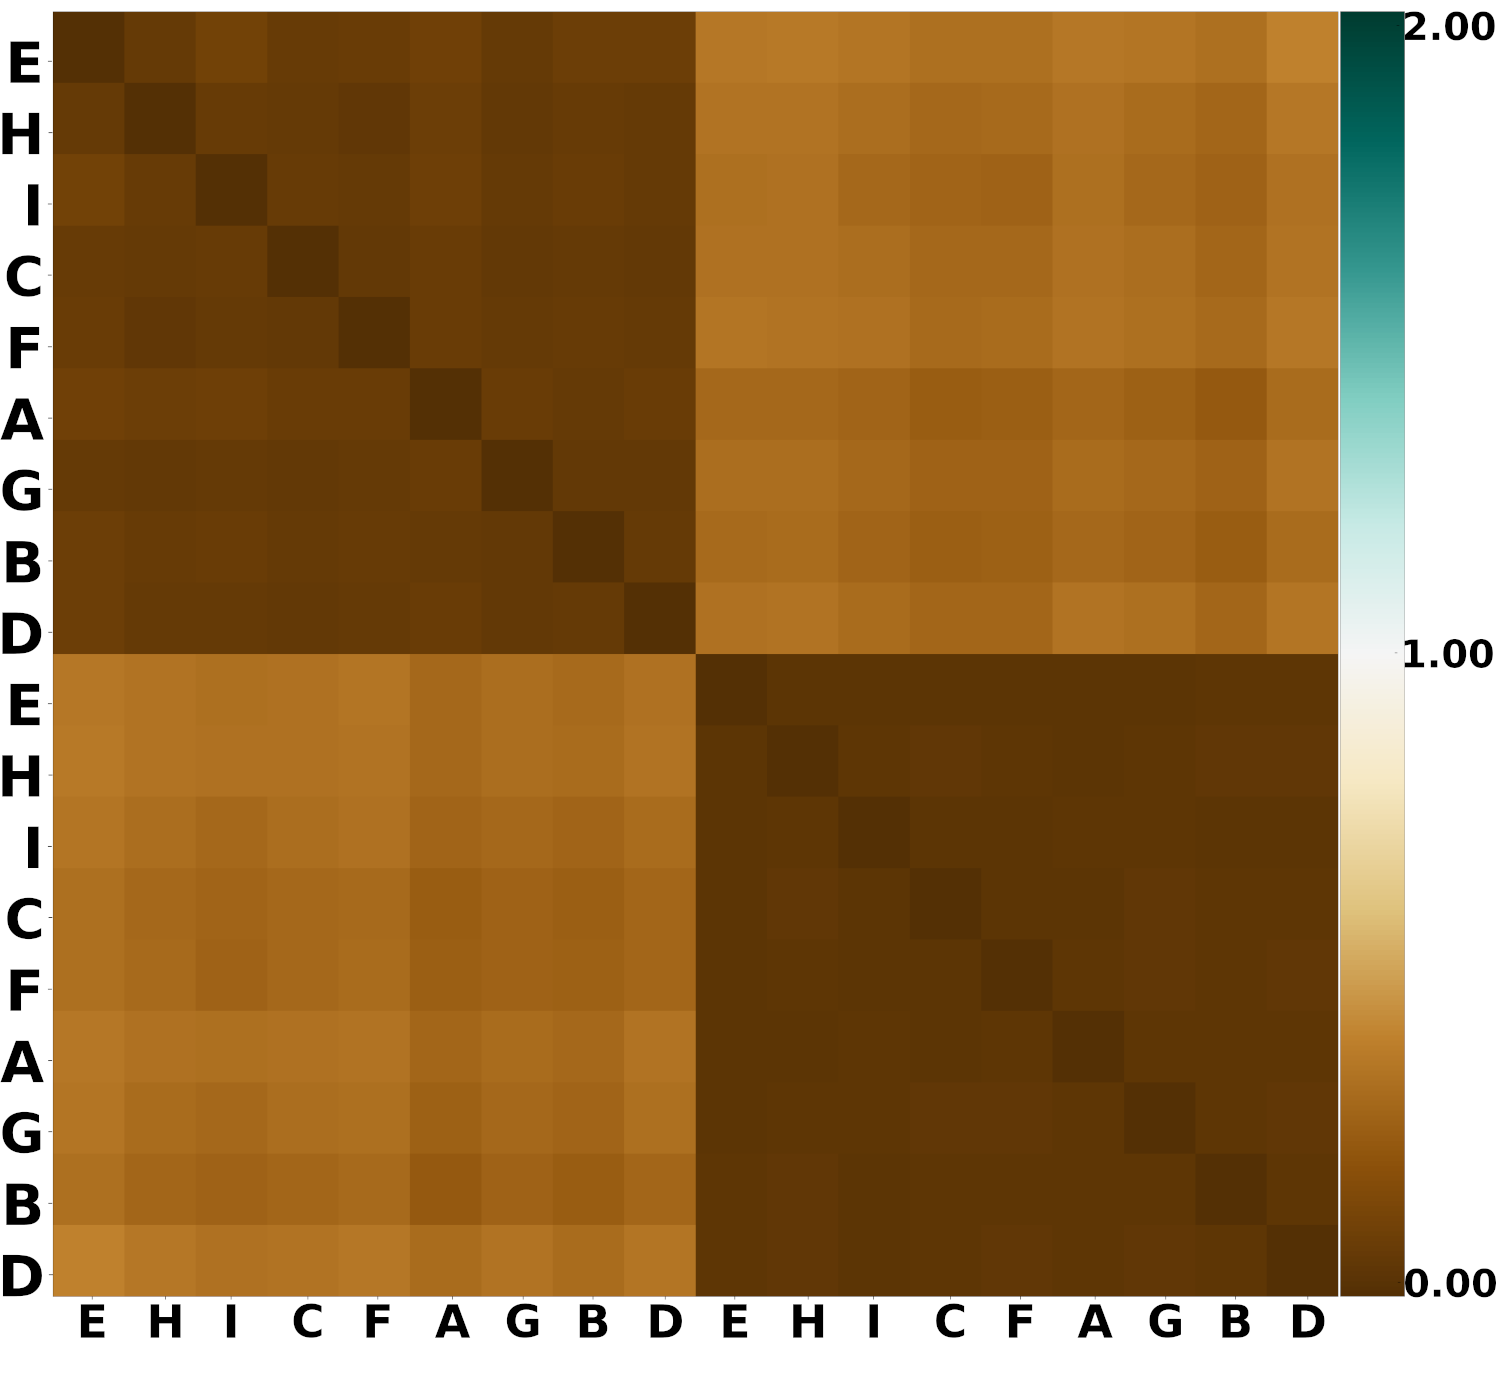
\includegraphics[width=\textwidth]{memento/srm/group_avg-transformed_transformed-n-5-avg-test_trialdist-18_order-probability.png}
		\caption{$k=5$}
		\label{fig:shared5}
	\end{subfigure}
	\begin{subfigure}{0.18\textwidth}
		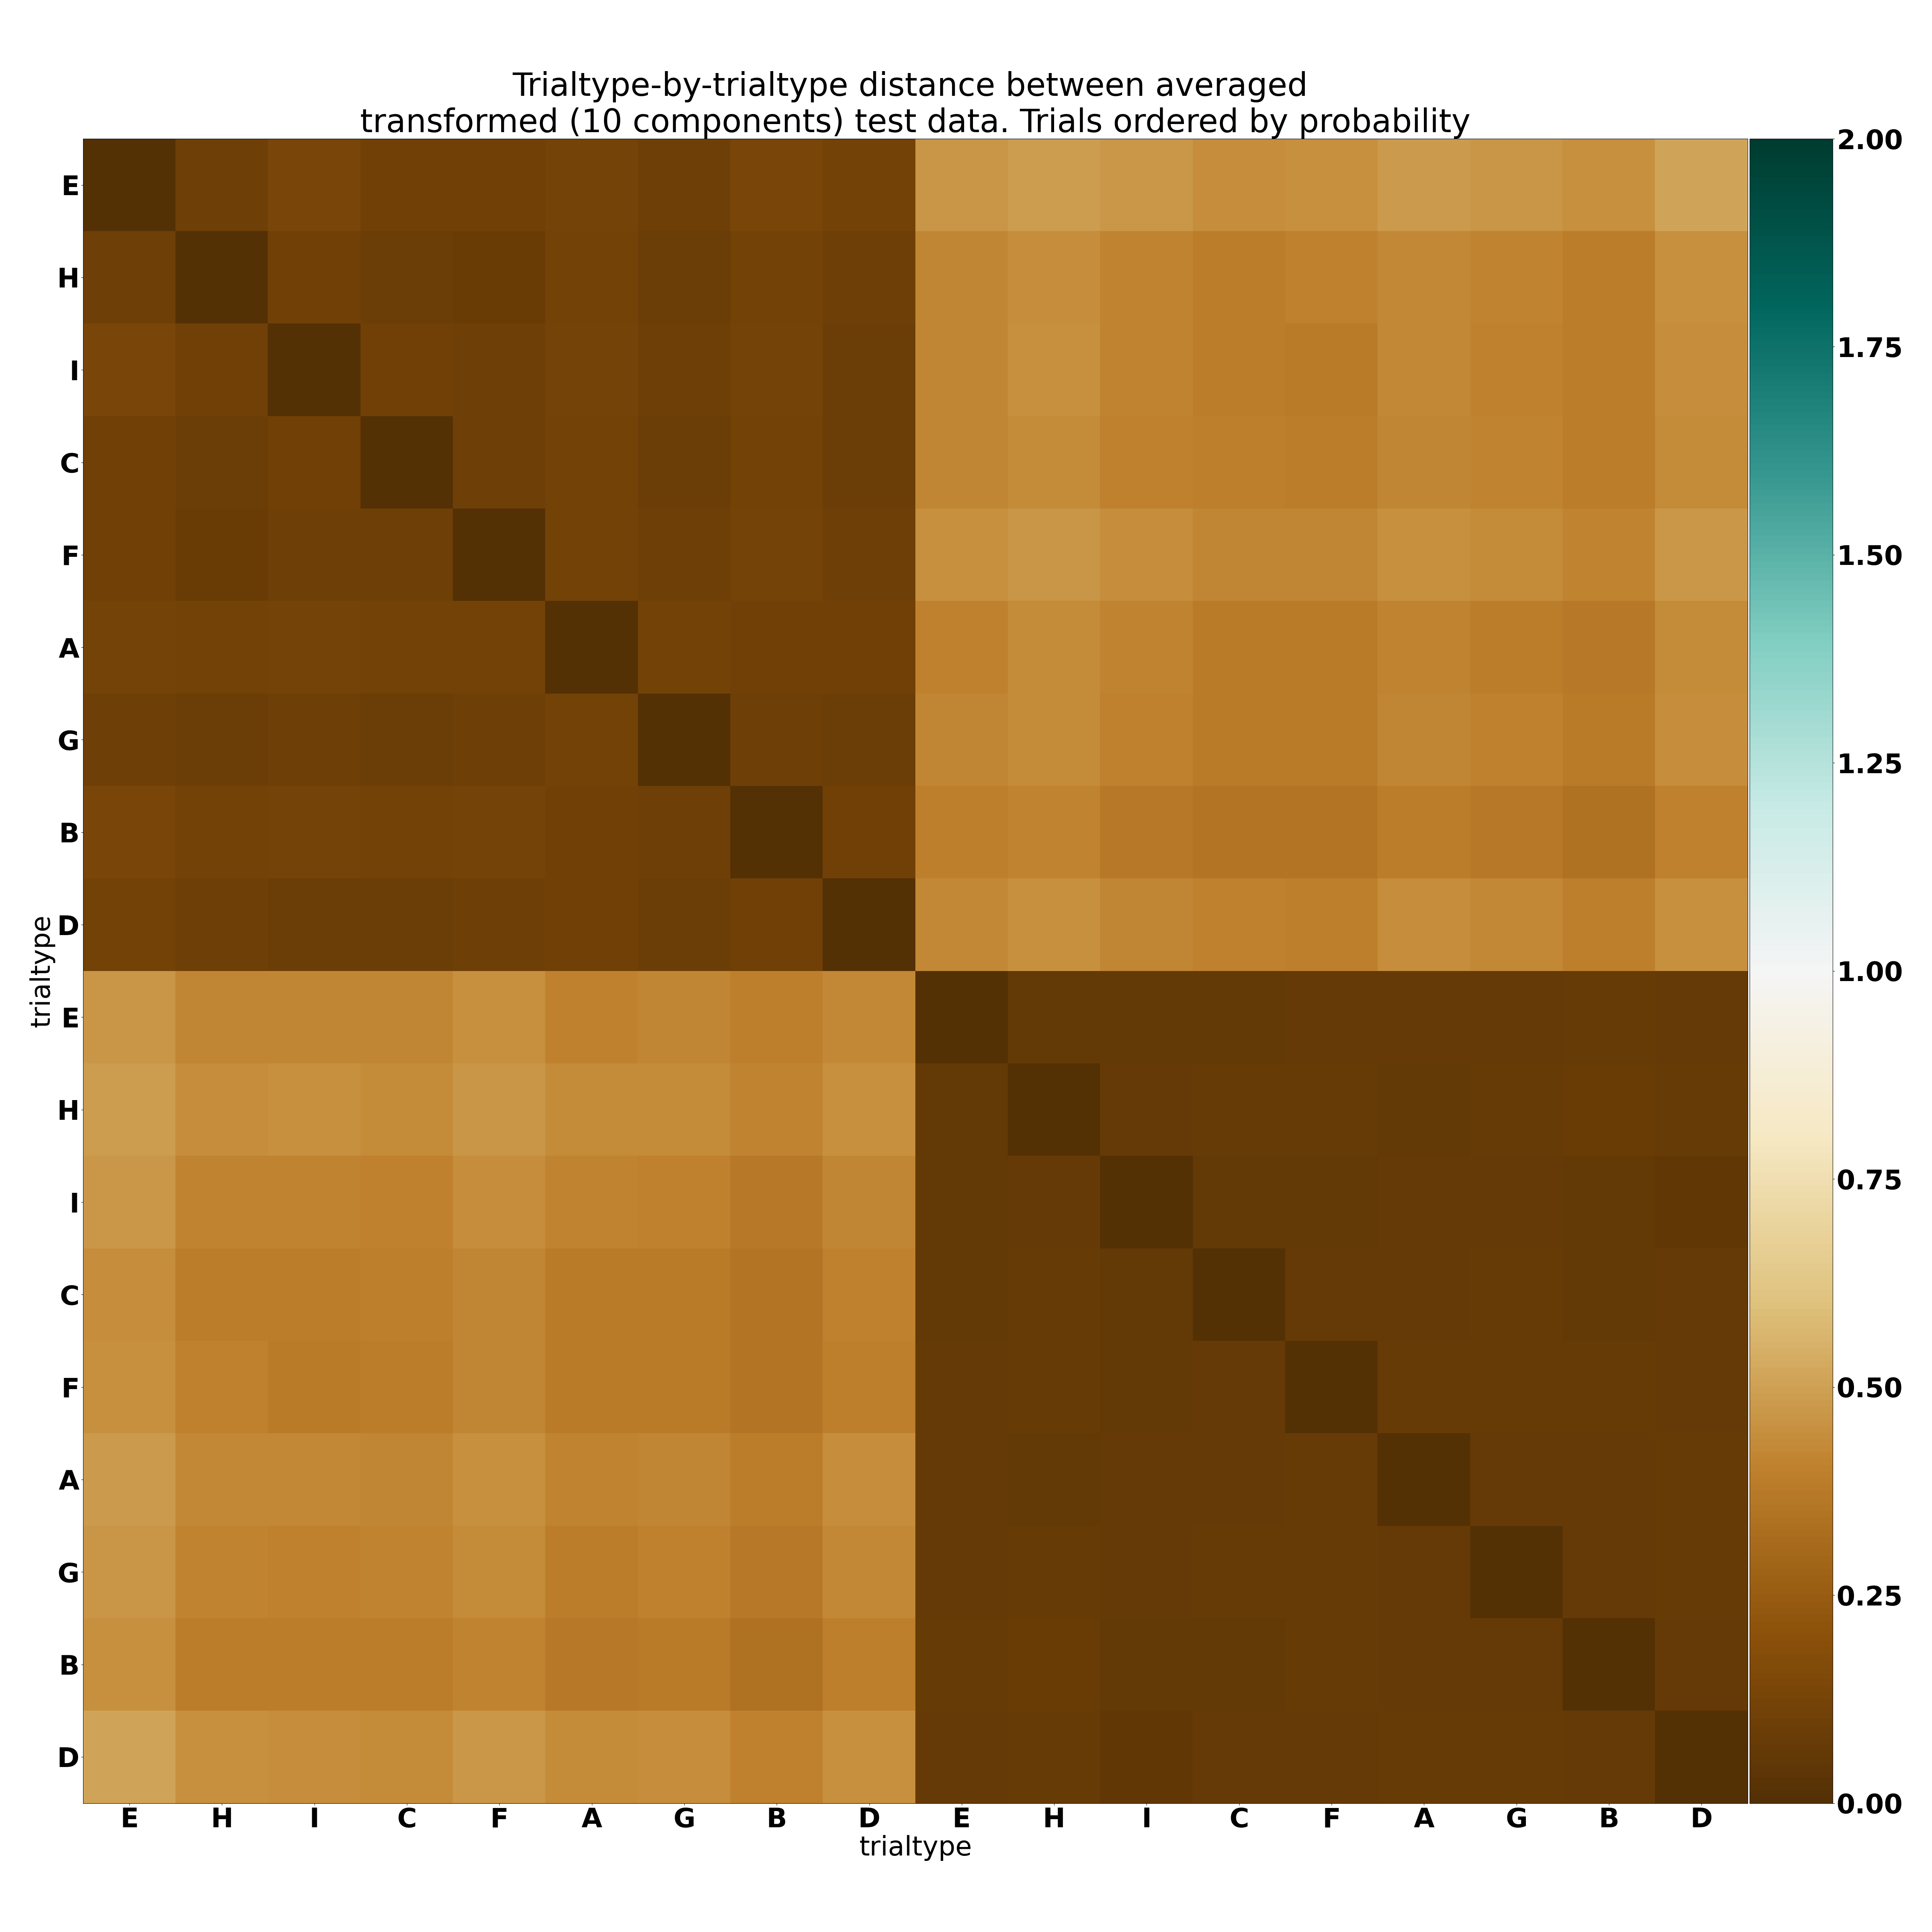
\includegraphics[width=\textwidth]{memento/srm/group_avg-transformed_transformed-n-10-avg-test_trialdist-18_order-probability.png}
		\caption{$k=10$}
		\label{fig:shared10}
	\end{subfigure}
	\begin{subfigure}{.18\textwidth}
		\includegraphics[width=\textwidth]{memento/srm/group_avg-transformed_transformed-n-20-avg-test_trialdist-18_order-probability.png}
		\caption{$k=20$}
		\label{fig:shared20}
	\end{subfigure}
	\begin{subfigure}{0.18\textwidth}
		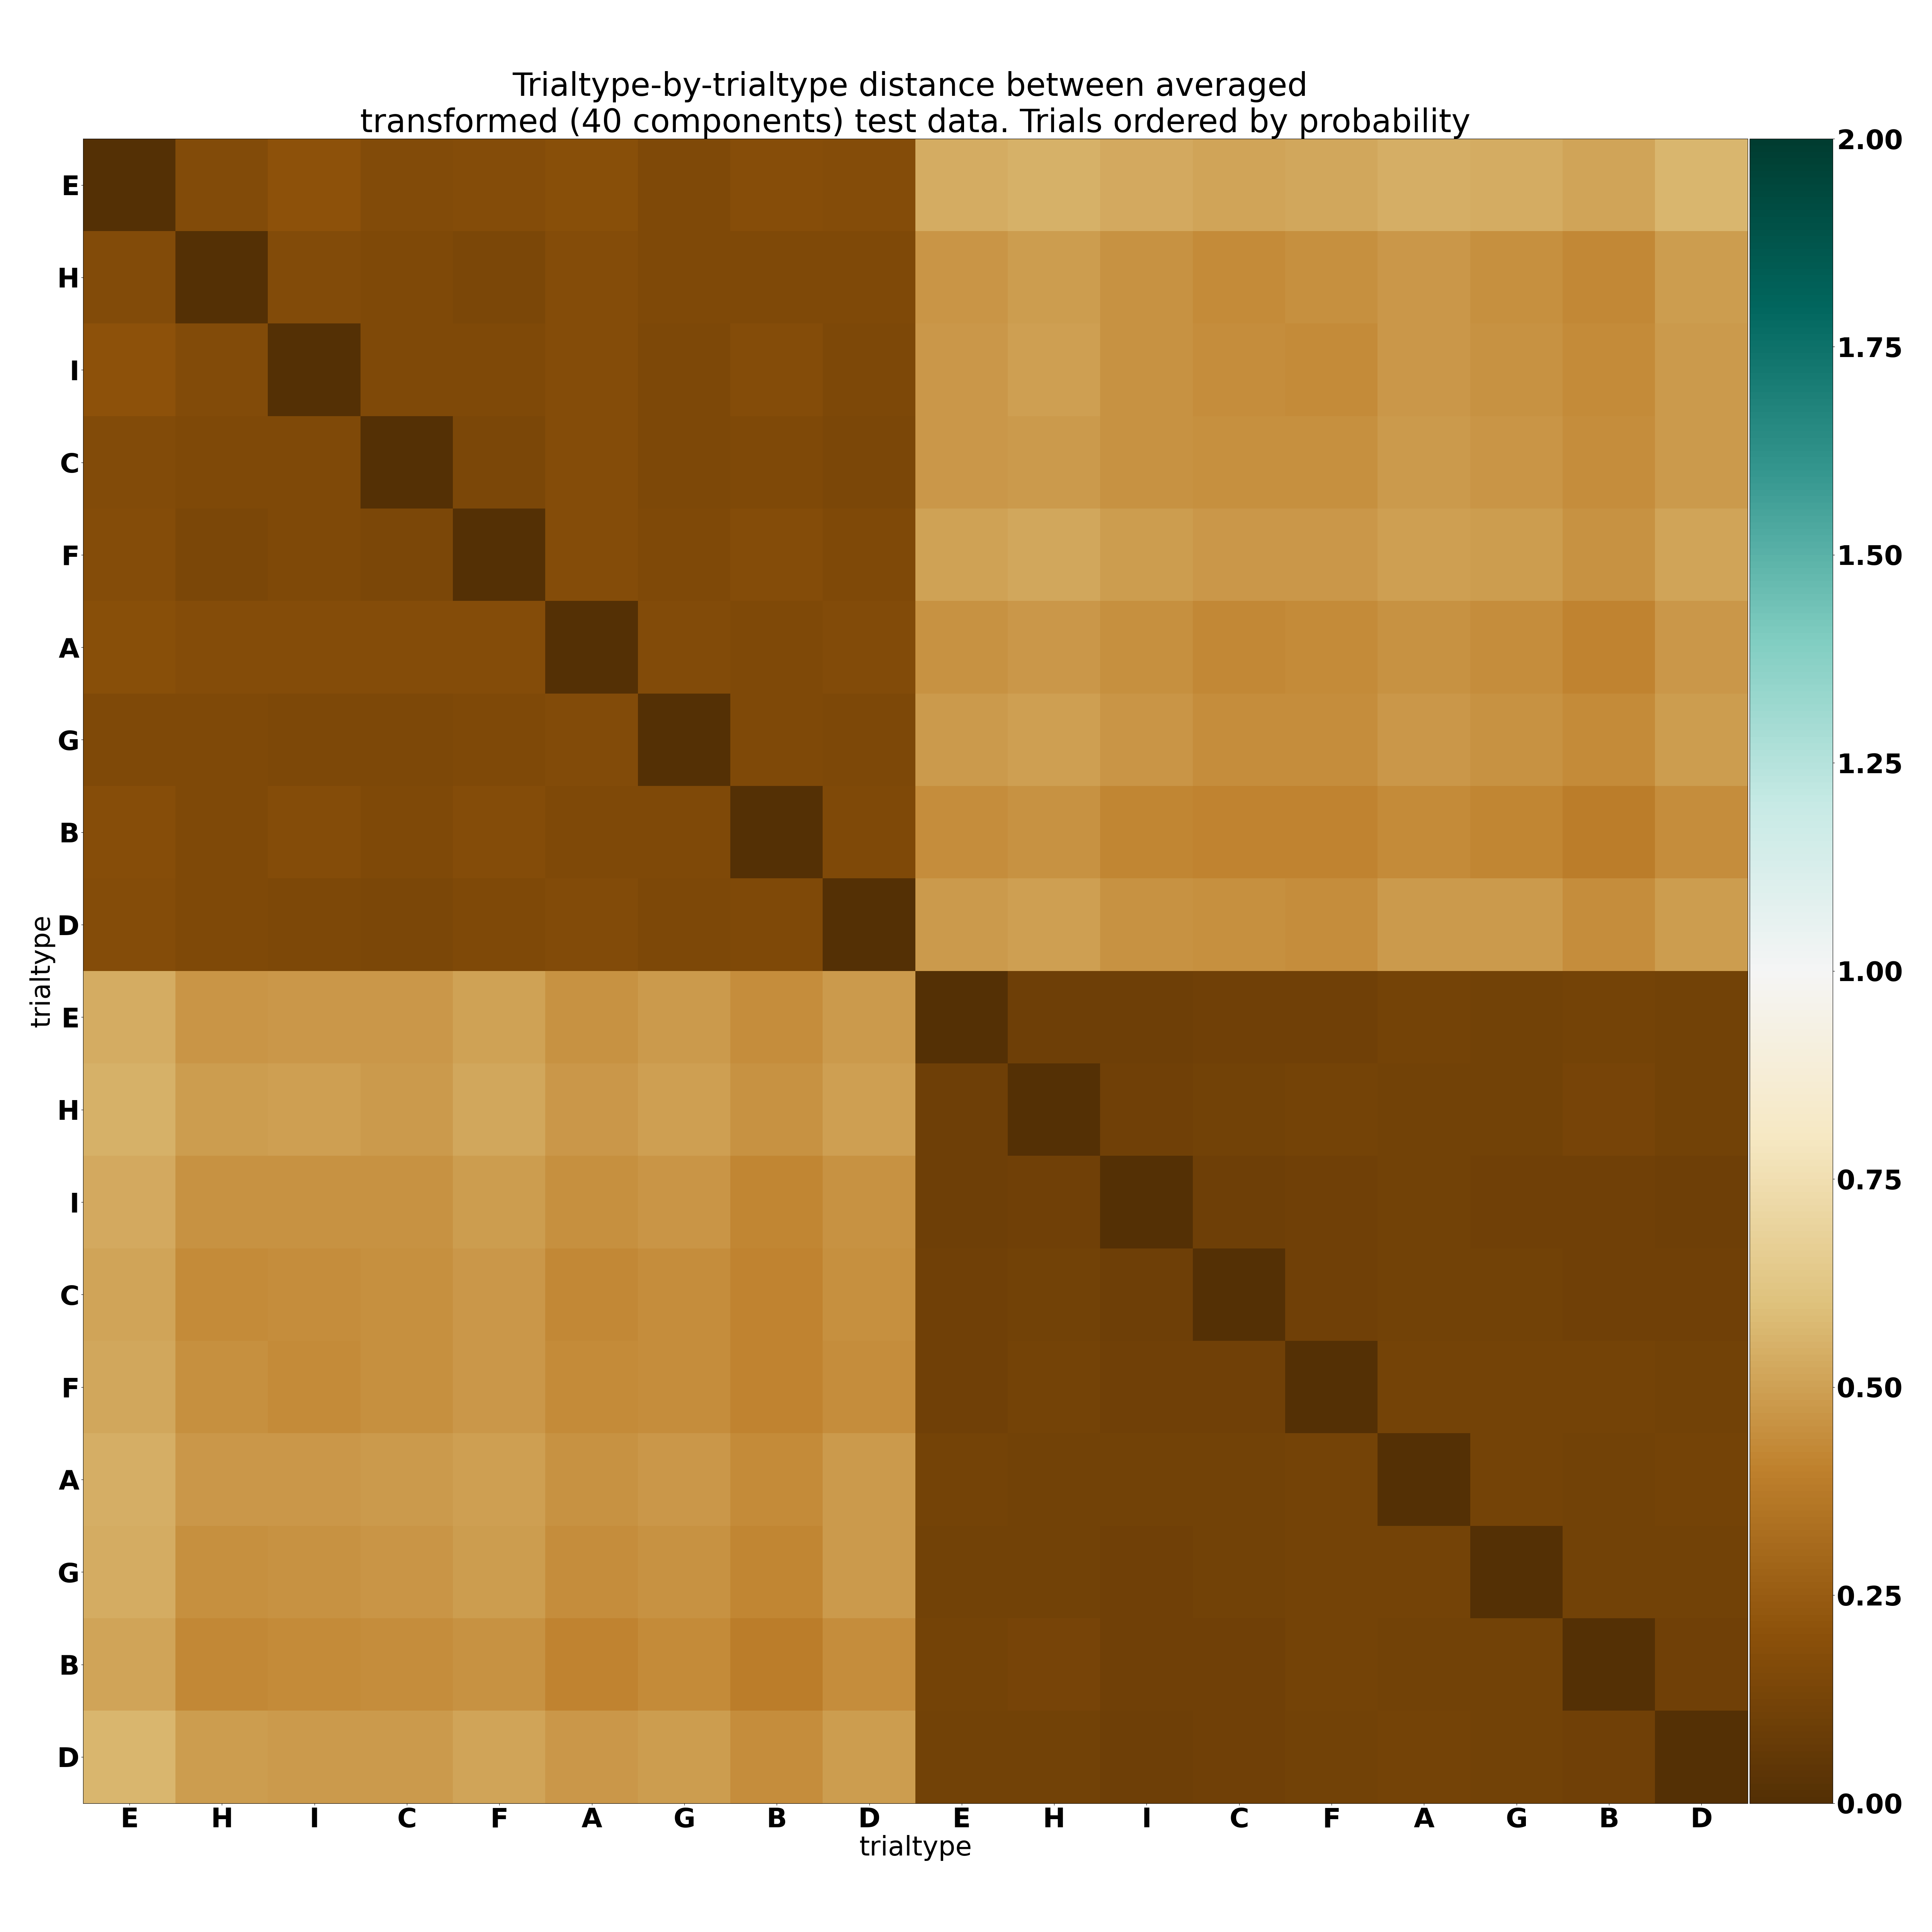
\includegraphics[width=\textwidth]{memento/srm/group_avg-transformed_transformed-n-40-avg-test_trialdist-18_order-probability.png}
		\caption{$k=40$}
		\label{fig:shared40}
	\end{subfigure}
	\begin{subfigure}{0.18\textwidth}
		\includegraphics[width=\textwidth]{memento/srm/group_avg-transformed_transformed-n-80-avg-test_trialdist-18_order-probability.png}
		\caption{$k=80$}
		\label{fig:shared80}
	\end{subfigure}
	%\newline
	\caption[Transformed test data in shared space]{Similarity of time courses from different stimulus options in shared space. Test data is transformed into the shared space using subject-specific basis of the \gls{SRM}, averaged across subjects. As correlation distances do not follow a normal distribution, individual distance matrices were Fisher-Z-transformed prior to averaging and transformed back to correlation distance afterwards.}
	\label{fig:srmtransformedspaces}
\end{figure}

%\begin{figure}
%	\centering
%	\begin{subfigure}{.18\textwidth}
%		\includegraphics[trim={0.7cm 0.3cm 1cm 11cm},clip,width=\textwidth]{memento/srm/sub-001_corr-dist_transformed-avg-testdata_full-stim_order-probability.png}
%		\caption{sub-001}
%		\label{fig:transformed001}
%	\end{subfigure}
%	\begin{subfigure}{0.18\textwidth}
%		\includegraphics[trim={0.7cm 0.3cm 1cm 11cm},clip,width=\textwidth]{memento/srm/sub-002_corr-dist_transformed-avg-testdata_full-stim_order-probability.png}
%		\caption{sub-002}
%		\label{fig:transformed002}
%	\end{subfigure}
%	\begin{subfigure}{.18\textwidth}
%		\includegraphics[trim={0.7cm 0.3cm 1cm 11cm},clip,width=\textwidth]{memento/srm/sub-003_corr-dist_transformed-avg-testdata_full-stim_order-probability.png}
%		\caption{sub-003}
%		\label{fig:transformed003}
%	\end{subfigure}
%	\begin{subfigure}{0.18\textwidth}
%		\includegraphics[trim={0.7cm 0.3cm 1cm 11cm},clip,width=\textwidth]{memento/srm/sub-004_corr-dist_transformed-avg-testdata_full-stim_order-probability.png}
%		\caption{sub-004}
%		\label{fig:transformed004}
%	\end{subfigure}
%	\begin{subfigure}{0.18\textwidth}
%		\includegraphics[trim={0.7cm 0.3cm 1cm 11cm},clip,width=\textwidth]{memento/srm/sub-005_corr-dist_transformed-avg-testdata_full-stim_order-probability.png}
%		\caption{sub-005}
%		\label{fig:transformed005}
%	\end{subfigure}
%	%\newline
%		\begin{subfigure}{.18\textwidth}
%		\includegraphics[trim={0.7cm 0.3cm 1cm 11cm},clip,width=\textwidth]{memento/srm/sub-006_corr-dist_transformed-avg-testdata_full-stim_order-probability.png}
%		\caption{sub-006}
%		\label{fig:transformed006}
%	\end{subfigure}
%	\begin{subfigure}{0.18\textwidth}
%		\includegraphics[trim={0.7cm 0.3cm 1cm 11cm},clip,width=\textwidth]{memento/srm/sub-007_corr-dist_transformed-avg-testdata_full-stim_order-probability.png}
%		\caption{sub-007}
%		\label{fig:transformed007}
%	\end{subfigure}
%	\begin{subfigure}{.18\textwidth}
%		\includegraphics[trim={0.7cm 0.3cm 1cm 11cm},clip,width=\textwidth]{memento/srm/sub-008_corr-dist_transformed-avg-testdata_full-stim_order-probability.png}
%		\caption{sub-008}
%		\label{fig:transformed008}
%	\end{subfigure}
%	\begin{subfigure}{0.18\textwidth}
%		\includegraphics[trim={0.7cm 0.3cm 1cm 11cm},clip,width=\textwidth]{memento/srm/sub-009_corr-dist_transformed-avg-testdata_full-stim_order-probability.png}
%		\caption{sub-009}
%		\label{fig:transformed009}
%	\end{subfigure}
%	\begin{subfigure}{0.18\textwidth}
%		\includegraphics[trim={0.7cm 0.3cm 1cm 11cm},clip,width=\textwidth]{memento/srm/sub-010_corr-dist_transformed-avg-testdata_full-stim_order-probability.png}
%		\caption{sub-010}
%		\label{fig:transformed010}
%	\end{subfigure}
%	\caption[Test data transformed into the shared space]{Test data from the first ten participants, transformed into the shared space}
%	\label{fig:transformedspaces}
%\end{figure}

One potential reason for this is that the potentially subtle differences between stimulus types were not prominent enough to be reflected strongly in the shared spaces, and signals corresponding to more general cognition, such as generic visual processing, dominated instead.
To investigate whether features corresponding to the trial structure in general are preserved during \gls{SRM}, I used the shared response space generated over the entire trial course to visualize the time point by time point similarity of the trial in shared space.
This analyses mirrored the previous approach, but epochs were not split by stimulus type and pooled instead, and the correlation distance was not calculated between time series, but between $k$ features per time point.
The result is visualized for three different values of $k$ in Figure \ref{fig:srmsharedspacetrial}.
The trial structure, in particular marked differences between the first stimulus, the delay phase, and the second stimulus, are visible for shared spaces of all dimensionalities.
With growing dimensionality $k$, similarities and dissimilarities decrease, which can be expected given that larger dimensionality values extend the vectors between which correlation distance is calculated, and can also be observed with increasing dimensionality in the previous shared spaces.
While individual stimulus-type differences did not emerge in the shared space, the \gls{SRM} was nevertheless able to capture trial-course induced differences.

\begin{figure}
	\centering
	\begin{subfigure}{0.32\textwidth}
		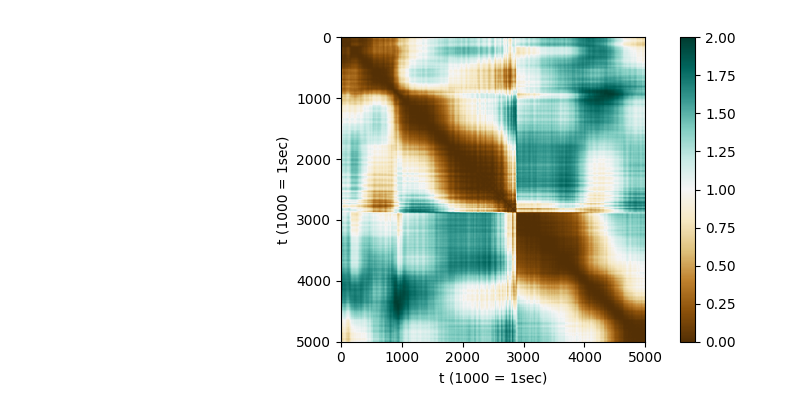
\includegraphics[width=\textwidth]{memento/srm/task-memento_srm-5_fulltrial_distances.png}
		\caption{$k$=5}
	\end{subfigure}
	\begin{subfigure}{0.32\textwidth}
		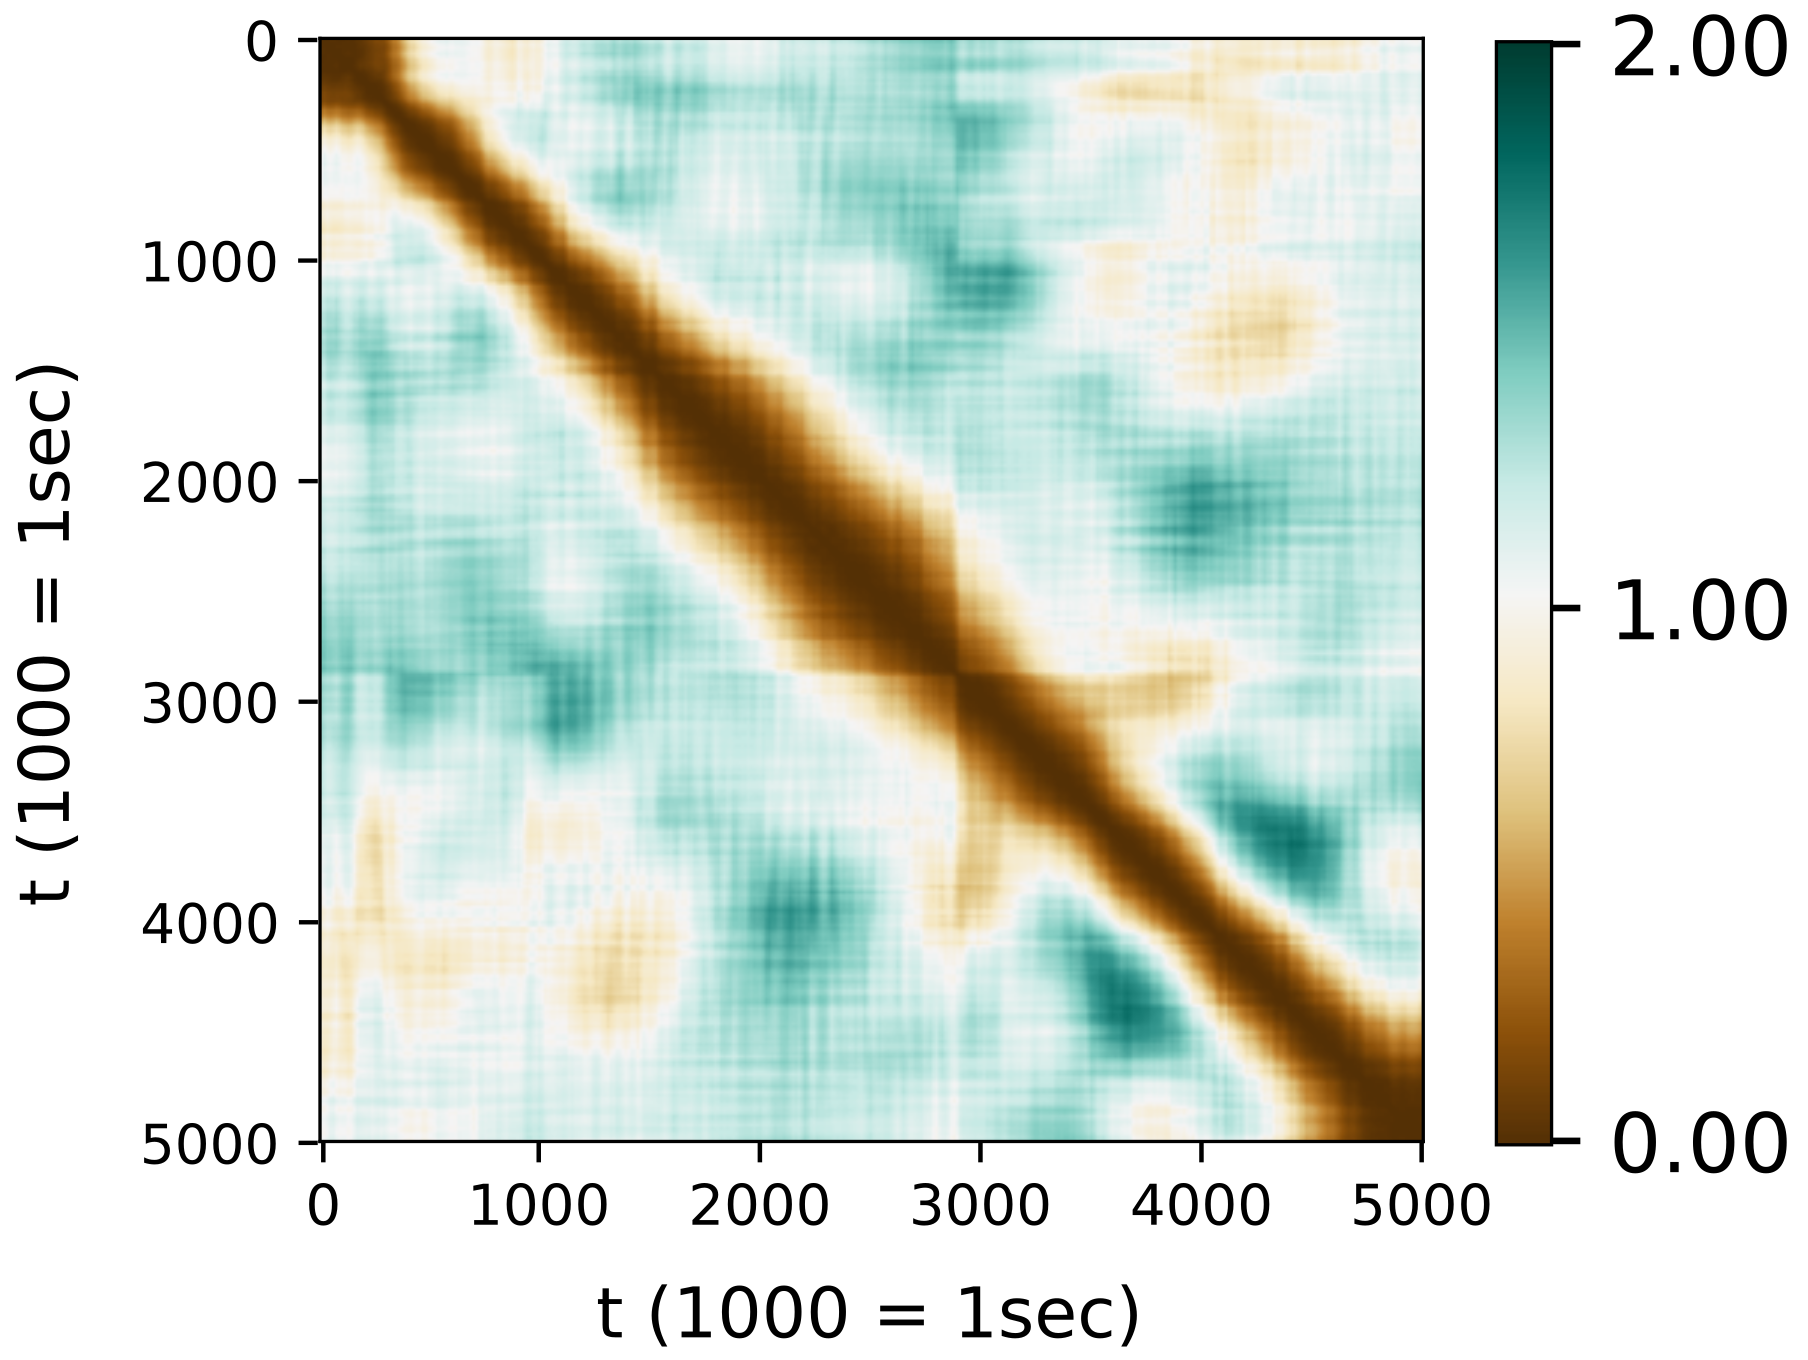
\includegraphics[width=\textwidth]{memento/srm/task-memento_srm-10_fulltrial_distances.png}
		\caption{$k$=10}
	\end{subfigure}
	\begin{subfigure}{0.32\textwidth}
		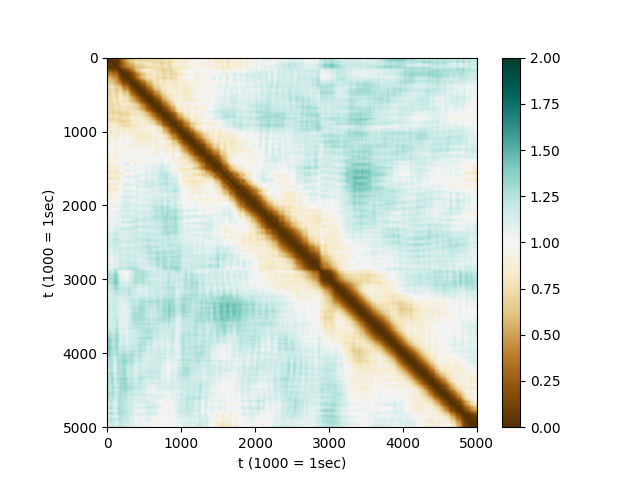
\includegraphics[width=\textwidth]{memento/srm/task-memento_srm-20_fulltrial_distances.png}
		\caption{$k$=20}
	\end{subfigure}
	\caption[Time point by time point correlation distances in shared spaces]{Time point by time point correlation distances in shared spaces build from the entire trial, across epochs with different stimulus types, for different values of $k$. Notable events in the trial, such as the stimulus presentation (0-700ms, 2700-3400ms) or the delay phase (700-2700ms) emerge as patterns.}
	\label{fig:srmsharedspacetrial}
\end{figure}


%For this reason, most applications of functional alignment use feature-rich, naturalistic stimulation such as movies \citep{haxby2020hyperalignment,bazeille2021empirical}.
%Nevertheless, the cleaned epochs from the experiment can be brought into a standardized order to meet this assumption \citep{chentutorial}.

%In a recent comparison of functional alignment methods, \gls{SRM} yielded the highest decoding accuracy gains on naturalistic \gls{fMRI} data \citep{bazeille2021empirical}.
%\citep{janati2020multi} employed functional alignment to perform source reconstruction.
%\gls{SRM} is successfully and widely used with fMRI data \citep{bazeille2021empirical}, in particular for naturalistic acquisitions with free-viewing tasks and movie stimuli (cite Sam).
%More rarely, the method is used in experimental paradigms the method is only rarely used in \gls{meg} or trial-based experimental designs.
%\citet{kalyani2023reduced} used shared response modeling to decode somatosensory finger maps, and changes in their representation with age.
%\citet{xie2021minimal} employed the method to functionally align intracranial EEG recordings.
%Thus the methods' utilities was first tested with a number of analyses intended to serve as sanity checks.

%\begin{figure}
%	\centering
%	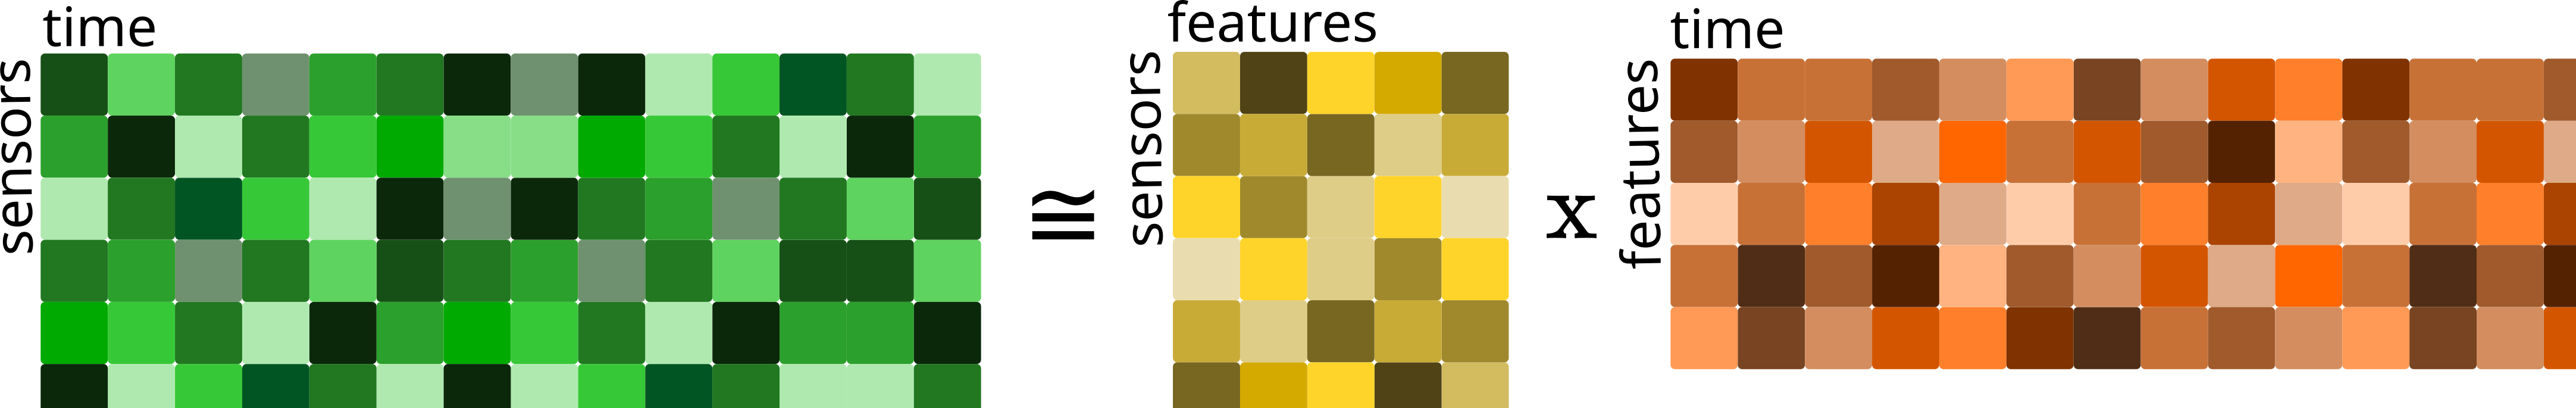
\includegraphics[width=0.9\textwidth]{memento/srm/srm_basics_1.png}
%	\caption[SRM overview]{\gls{meg} data can be represented as a matrix. In \gls{SRM} on \gls{meg} data, sensor-by-time matrices are decomposed into a orthogonal subject specific basis matrix (sensor-by-features), a common shared feature matrix (features-by-time), and a subject-specific error}
%	\label{fig:srm-basics}
%\end{figure}

\subsection{Shared response modeling in spectral space}

In further analyses, I investigated delay and decision periods of the trial.
In comparison to the trial phases with visual stimulation, neural activity in these periods should be driven less by external visual stimuli, but rather by internal cognitive processes related to working memory maintenance, motor preparation, or decision making.
The distribution of reaction times in the task (see Figure \ref{behavioral-analysis}), however, revealed different processing speeds, evident in intra- and inter-individual variation in response time.
Therefore, even if participants showed similar cognitive processes during the trial that \gls{SRM} could detect, their temporal characteristics likely vary considerably across trials and subjects.
Thus, given the explicit requirement of temporal synchronicity for functional alignment and the high temporal resolution of \gls{meg}, this could pose a challenge.
To use the shared response model nevertheless, I utilized the flexibility with which the \gls{SRM} method allows transformations between idiosyncratic and shared neural spaces, and trained the model with input data in a space without timing information.
For this, I drew inspiration from spectral analysis.\\
Spectral analysis consists of deconstructing a time domain signal of a given length into its constituent oscillatory components using Fourier analysis.
MEG signal consists of oscillations with an amplitude, a frequency, and a phase.
Frequency, usually measured in hertz (Hz), is the number of times a specified event occurs within a specified time interval, while amplitude is the height, force or power of the wave, and power is the squared amplitude.
Phase involves the relationship between two or more signals that share the same frequency and describes the relationship between the position of the amplitude crests and troughs of two waveforms, measured in distance, time, or degrees.
If the peaks of two signals with the same frequency are in exact alignment at the same time, they are said to be in phase and out of phase otherwise.
If the exact timing or duration of shared activity in question is subject to intra- and inter-individual variation, it is not necessarily phase-locked.
However, a spectral decomposition of this signal results in power spectrum, with the frequency domain of the oscillations on the x axis, and the amplitude on the y axis.
Typically, these transformations are used in time-frequency analyses to investigate the progression of \gls{meg} power in different frequency bands of interest over time \citep{hari2017primer}.
However, in the upcoming analyses I used them to expressed signal as a function of frequency rather than time and use the transformation from a time-resolved representation of data to a representation in the frequency domain to find shared signals with different temporal signatures.
Importantly, the model bases of an \gls{SRM} assign weights to sensors regardless of whether they contribute to a shared signal in time-resolved or spectral space.
Therefore, I can fit a shared response model on spectral data to find shared frequency components, but then use the model bases to transform time-resolved data (see Figure \ref{fig:spectral-srm}).
This not only allows the visualization of shared components as a time series, but also easier interpretation of components in the context of the experimental paradigm.
To evaluate the feasibility of this novel method, I first conducted a simulation study.

\begin{figure}
	\centering
	\begin{subfigure}{0.9\textwidth}
		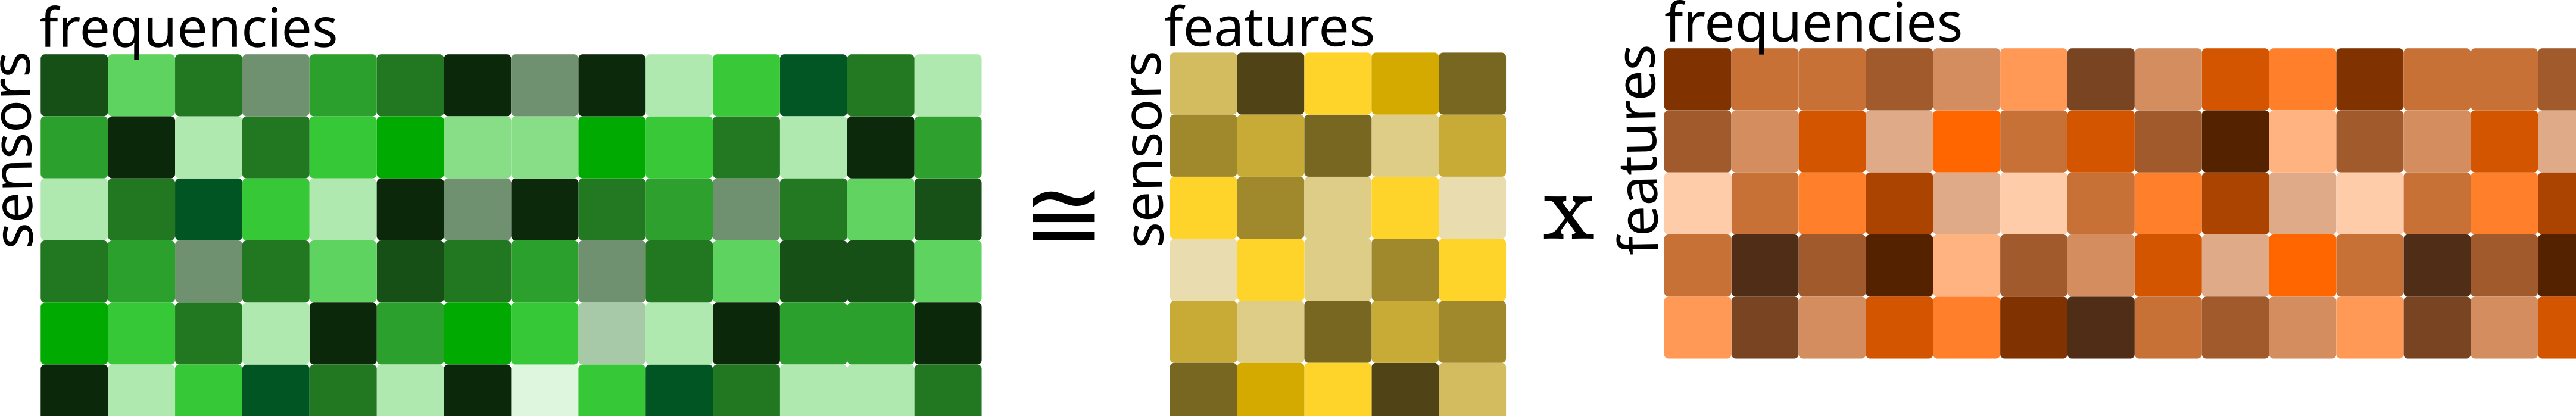
\includegraphics[width=\textwidth]{memento/spectral_srm/spectral_srm_basics_1.png}
		\caption{Fitting the shared response model on spectral data}
		\label{fig:spectral-srm1}
	\end{subfigure}
	\begin{subfigure}{0.9\textwidth}
		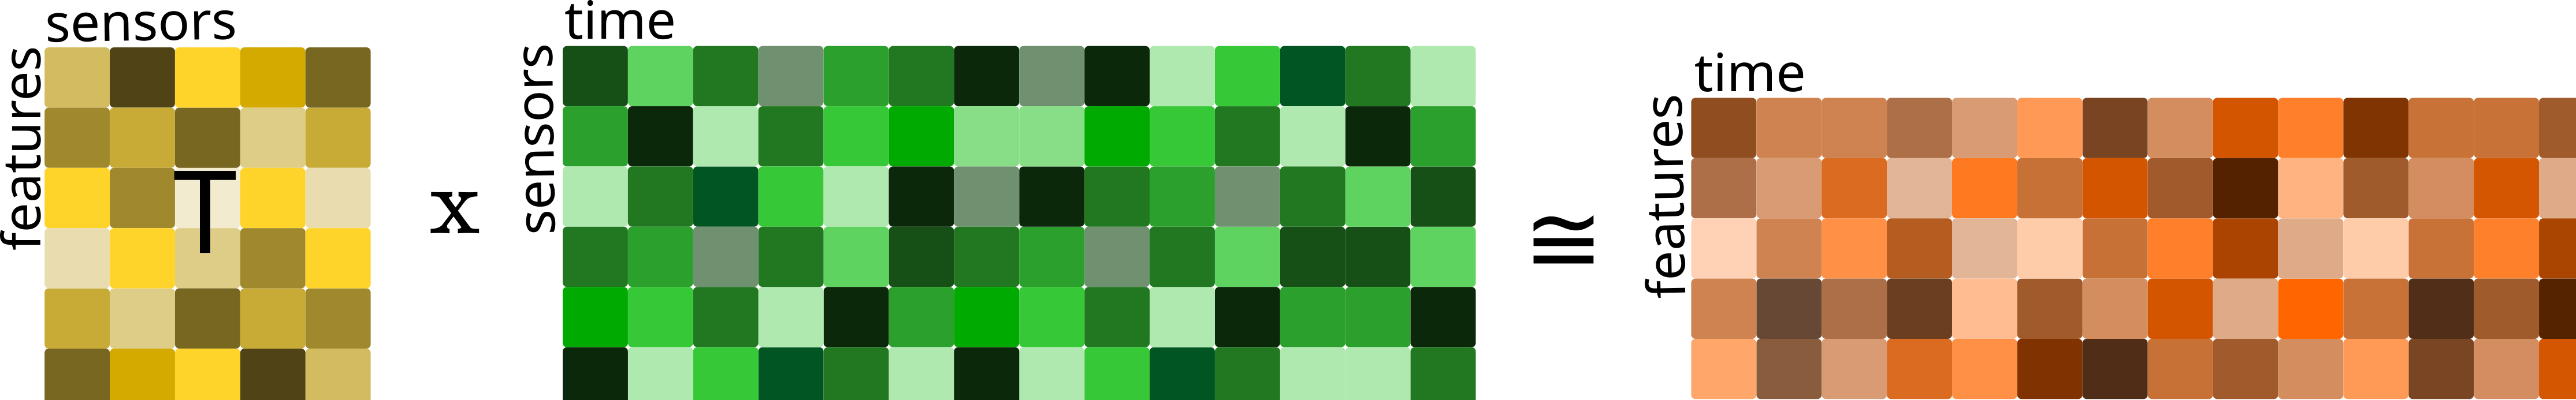
\includegraphics[width=\textwidth]{memento/spectral_srm/spectral_srm_basics_2.png}
		\caption{Transforming time resolved data into the shared space}
		\label{fig:spectral-srm2}
	\end{subfigure}
	\caption[Spectral shared response modeling]{Spectral shared response modeling: A shared response model decomposes spectral neural data (\ref{fig:spectral-srm1}, green) into a shared spectral space (features by frequencies; orange) and subject-specific basis (sensors by features; yellow). Because the subject specific bases transform sensor data independent on whether it is time resolved or spectral, they can be used to transform time resolved data (\ref{fig:spectral-srm2}; green) into time courses of the shared response spaces features. Capital ``T'' denotes a matrix transpose.}
	\label{fig:spectral-srm}
\end{figure}

\begin{figure}[H]
	\begin{subfigure}{1\textwidth}
		\centering
		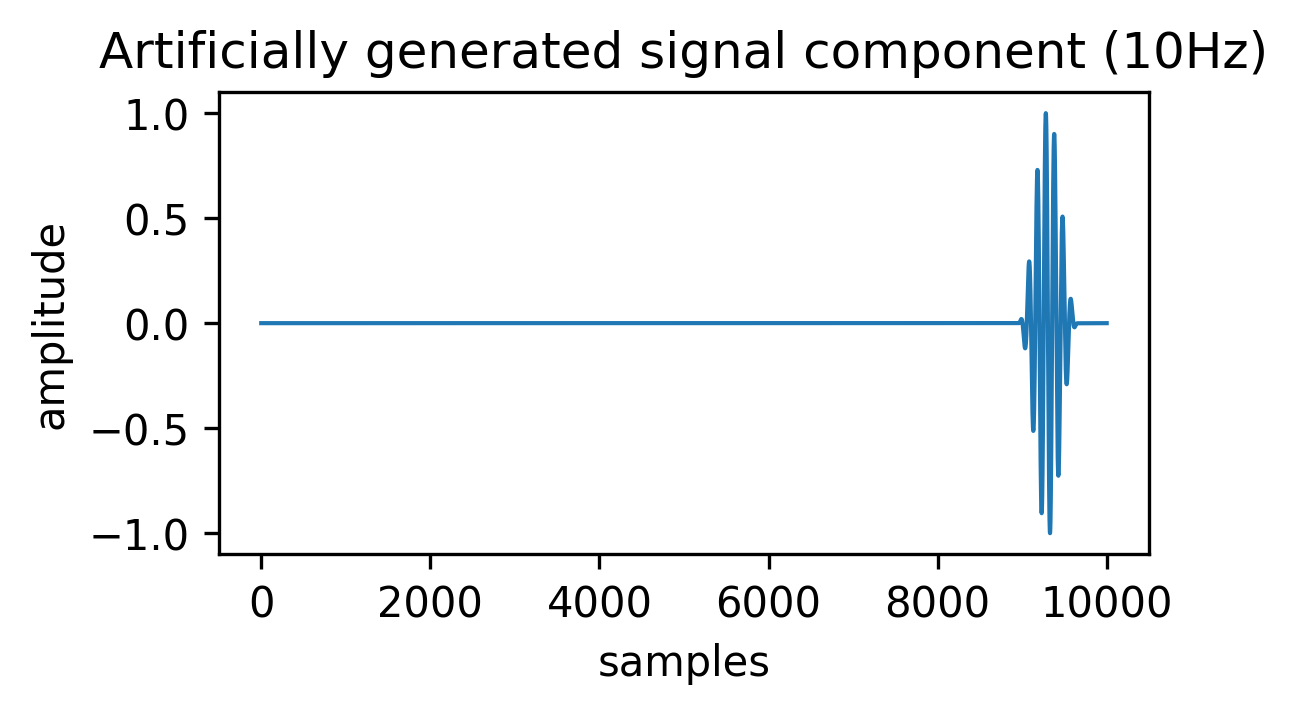
\includegraphics[trim={0 0 0 0.7cm},clip,width=.48\textwidth]{memento/simulation/sim_2.png}
		\includegraphics[trim={0 0 0 0.7cm},clip,width=.435\textwidth]{memento/simulation/sim_10.png}
	\end{subfigure}
	\caption[Artificial signal for simulation]{Artificial signal (10~000 samples) with a 1000 sample spanning 10Hz main frequency component (left), and partially embedded into 306 sensors with Gaussian noise (right). 20 percent of sensors contain the main signal in varying amounts, mirroring how brain signals are only present in certain sensors and decrease in strength over distance.}
	\label{fig:sim_artificial_signal}
\end{figure}

\subsection{Simulation study}


To simulate \gls{meg} data, I generated a ``ground truth'' signal with a given frequency and wave form, and embedded it partially into 306 artificial sensors with Gaussian noise (Figure \ref{fig:sim_artificial_signal}).
To mirror how brain signals are only present in certain sensors and with varying strengths, only a fixed amount of sensors received the signal.
For each sensor with a signal, a random weight between is drawn that determines the strength with which the signal is scaled.
This is repeated for $N = 30$ artificial subjects, but with a different random phase offset in the signal for each to simulate data from several subjects with a common frequency component that occurs at different points in time.
If the \gls{SRM} is successful, the shared response should reflect the ground truth signal despite phase offsets, and the subject-specific model bases should reflect the magnitudes of the weights for each sensor.\\
Using this artificial data as the basis for shared response modeling, I fitted a probabilistic \gls{SRM} with $k=10$ features to recover the signal as a shared component - either on time resolved data, or after transforming the data into its frequency spectrum.\\
When fit on time resolved data with phase shifts, the resulting shared space consists of components that differentially picked up signals from one or more participants, but represent it in a time series of repeated or overlapping signals.
This makes an interpretation of individual components difficult (Figure \ref{fig:sim-timeresolved-shared}).
The sensor weights that the model estimates for each component also do not show a clear association with the true weights used in the generation of the artificial data (Figure \ref{fig:sim-timeresolved-weights}).
In other words, with phase shifts between individual simulations' signals, different components of the shared space capture several participants' signals, but no \textit{general} ground truth signal.
However, transforming the signal into its frequency components, the spectral space, removes timing information, and with it, the phase offsets.
While the components in spectral space are not easy to interpret or differentiate (see Figure \ref{fig:sim-spectral-shared}), the scatterplot reveals that certain components' weights show a clear association to the weights used for model generation \ref{fig:sim-spectral-weights}.
\begin{figure}[H]
	\centering
	\begin{subfigure}{0.35\textwidth}
		\includegraphics[width=\textwidth]{memento/simulation/model-weights_versus_ground-truth_all-ds.png}
		\caption{SRM on time-resolved data}
		\label{fig:sim-timeresolved-weights}
	\end{subfigure}
	\begin{subfigure}{0.35\textwidth}
		\includegraphics[width=\textwidth]{memento/simulation/model-weights_versus_ground-truth_all-ds_spectral.png}
		\caption{SRM on spectral data}
		\label{fig:sim-spectral-weights}
	\end{subfigure}
	\caption[Relationship of model weights and true weights]{Recovered versus true model weights from an \gls{SRM} fitted on time resolved (left) or spectrally transformed data with phase shifts (right): Without spectral transformation, the relationship between model weights and ground truth weights appears mostly random. When fit on spectrally transformed data, the relationship between model weights and ground truth weights clearly captures an association for some of the $k=10$ components, indicating successful recovery the original weights.}
	\label{fig:sim-weights}
\end{figure}


This becomes apparent when shared components are visualized as time series by using the subject-specific weight matrices of the \gls{SRM} and individual subject's time-resolved data.
A few components consistently represent the original signal well across subjects, laying the basis for identifying shared signal in phase-shifted data and interpreting the shared components resulting from it.




\begin{figure}
	\centering
	\begin{subfigure}{.4\textwidth}
		\includegraphics[width=\textwidth]{memento/simulation/sim_3.png}
		\caption{Shared space from time-resolved data}
		\label{fig:sim-timeresolved-shared}
	\end{subfigure}
	\begin{subfigure}{.43\textwidth}
		\includegraphics[width=\textwidth]{memento/simulation/sim_5.png}
		\caption{Shared space from spectral data}
		\label{fig:sim-spectral-shared}
	\end{subfigure}
	\centering
	\begin{subfigure}{1.\textwidth}
		\centering
		\includegraphics[trim={0 0.7cm 0 2.5cm},clip,width=.45\textwidth]{memento/simulation/spectral_srm_timeresolved_transformed_sub-001.png}
		\includegraphics[trim={0 0.7cm 0 2.5cm},clip,width=.45\textwidth]{memento/simulation/spectral_srm_timeresolved_transformed_sub-002.png}
		\caption{Shared components from \ref{fig:sim-timeresolved-shared} (visualized via transformation, for two ``subjects'')}
		\label{fig:sim-resolved-transformed}
	\end{subfigure}
	\centering
	\begin{subfigure}{1.\textwidth}
		\centering
		\includegraphics[trim={0 0.7cm 0 2.5cm},clip,width=.45\textwidth]{memento/simulation/spectral_srm_spectral_transformed_sub-001.png}
		\includegraphics[trim={0 0.7cm 0 2.5cm},clip,width=.45\textwidth]{memento/simulation/spectral_srm_spectral_transformed_sub-002.png}
		\caption{Shared components from \ref{fig:sim-spectral-shared} (visualized via transformation, for two ``subjects'')}
		\label{fig:sim-shared-transformed}
	\end{subfigure}

	\caption[Properties of a shared time-resolved or spectral space]{Properties of a shared time-resolved or spectral space. a) visualizes the shared space of a model fit on time-resolved data: Gaussian noise is reduced and signal of interest is retained, but signals from several subjects emerge as consecutive or overlapping activity. Using individual subject's weight matrices and raw data to visualize individual model components reveals that the signal of interest is not represented in the same components across two subjects (c). In comparison, b) shows the shared spectral space, and d) its transformed components. The components in shared space are spectral and difficult to interpret. But the strength with which components capture the signal of interest is consistent in the transformations with time-resolved data.}
	\label{fig:sim-spectral}
\end{figure}



\pagebreak
\subsection{Visualizing shared components}

After the simulation study demonstrated feasibility of the method, I subsequently applied it to the neural \gls{meg} recordings.
The underlying aim was to find shared components that represented decision-related or -relevant properties.
Unlike the previous \gls{SRM} analyses, models were trained with data from all participants.
Using the subject-specific bases, the time-resolved test data was then transformed in the shared space while retaining the temporal resolution (\ref{fig:spectral-srm2}) to visualize the components that the shared response model found.
The resulting components are thus time series.
I fit different models for different time slices of a trial, namely the first stimulus presentation, the delay phase, and the decision and feedback phase.
A subset of these visualizations are shown to illustrate the results for shared response models fit with $k = 5$ in Figure \ref{fig:spectral-comps-plain}.


\begin{figure}[H]
	\begin{subfigure}{0.33\textwidth}
		\includegraphics[width=\textwidth]{memento/spectral_srm/avg-signal_shared-shape_spectral-srm_5-feat_per-comp_visual.png}
		\caption{First stimulus presentation}
		\label{fig:spectral-comp-visual}
	\end{subfigure}
	\begin{subfigure}{0.33\textwidth}
		\includegraphics[width=\textwidth]{memento/spectral_srm/avg-signal_shared-shape_spectral-srm_5-feat_per-comp_delay.png}
		\caption{Delay period}
		\label{fig:spectral-comp-delay}
	\end{subfigure}
	\begin{subfigure}{0.33\textwidth}
		\includegraphics[width=\textwidth]{memento/spectral_srm/avg-signal_shared-shape_spectral-srm_5-feat_per-comp_response-locked.png}
		\caption{Decision and feedback}
		\label{fig:spectral-comp-decision}
	\end{subfigure}
	\caption[Shared components for different trial phases]{Time courses of shared components for different trial phases, as obtained by fitting a \gls{SRM} with $k=5$ features on spectrally transformed data. Each panel in each figure results from transforming left-out time-resolved epochs with the subject-specific base matrix for one component in the shared space and averaging the resulting transformations. Thus, each panel visualizes the time course of a functional topography identified with spectral \gls{SRM}. Depicted are three different trial phases, the first stimulus presentation, the delay phase, and the decision phase. In c), the dashed line indicates the motor response.}
	\label{fig:spectral-comps-plain}
\end{figure}


One possibility is that the modulation of these functionality topographies encodes different decision-related properties.
To investigate whether shared components differentially related to trial-specific attributes, unseen test data was transformed into the shared space, but visualized separately for trials with specific attributes.
For example, trials in which the first stimulus option had a different probabilities values were contrasted with each other.
I hypothesized that this could uncover shared components encoding stimulus properties, modulated via their amplitude.
To investigate this, I reused the models for visualizations of test data in various attribute splits.
A subset of these visualizations is shown in Figure \ref{fig:spectral-comps-attributes}.
They revealed that marked modulation differences only existed for splits between decisions, and those were only seen in shared spaces of the decision phase (Figure \ref{fig:spectral-comp-decision-splitchoice}).

\begin{figure}
	\begin{subfigure}{0.49\textwidth}
	\includegraphics[width=\textwidth]{memento/spectral_srm/trialtype-magnitude_avg-signal_shared-shape_spectral-srm_5-feat_per-comp_delay.png}
	\caption{Delay (split by stimulus probability)}
	\label{fig:spectral-comp-delay-splitprob}
\end{subfigure}
	\begin{subfigure}{0.49\textwidth}
		\includegraphics[width=\textwidth]{memento/spectral_srm/trialtype-probability_avg-signal_shared-shape_spectral-srm_5-feat_per-comp_delay.png}
		\caption{Delay (split by stimulus magnitude)}
		\label{fig:spectral-comp-delay-splitmag}
	\end{subfigure}
\hfill
	\begin{subfigure}{0.49\textwidth}
		\includegraphics[width=\textwidth]{memento/spectral_srm/event-choice_avg-signal_shared-shape_spectral-srm_5-feat_per-comp_delay.png}
		\caption{First stimulus presentation (split by choice)}
		\label{fig:spectral-comp-delay-splitchoice}
	\end{subfigure}
	\begin{subfigure}{0.49\textwidth}
		\includegraphics[width=\textwidth]{memento/spectral_srm/avg-signal_shared-shape_spectral-srm_5-feat_per-comp_response-locked_leftvsright.png}
		\caption{Decision (split by choice)}
		\label{fig:spectral-comp-decision-splitchoice}
	\end{subfigure}
	\caption[Shared components split by trial attribute]{Time courses of shared components, split by trial attributes. Shown are splits by the probability (a) and magnitude (b) of the first stimulus option during the delay phase, and splits by left or right choice during the presentation of the first option (c) and decision phase (d). In d), the dashed line indicates the motor response.}
	\label{fig:spectral-comps-attributes}
\end{figure}

\section{Decoding}
\label{decoding-analysis}

As previous analyses were unable to directly identify neural subspaces representing stimulus features, I turned to a multivariate method in the form of a temporal decoding analysis.
This method involves fitting a predictive model on each time instant within a trial, and evaluating the model performance at the same instant on new epochs \citep{king2018encoding}.
A temporal decoding analysis for the stimulus properties probability, magnitude, and expected value of the first stimulus option has already been performed by \citet{kaiserposter} in source space.
However, stimulus properties had above-chance decoding accuracies only during the stimulus presentation and a few hundred milliseconds into the delay period.
%In addition, above chance decoding succeeded in the time span of the second stimulus presentation, indicating an interesting reinstatement effect just prior to the motor response.
To investigate if dimensionality reduction methods including \gls{SRM} improved the decodability of stimulus properties in the delay period, I implemented a flexible temporal decoding pipeline that was able to employ different forms of dimensionality reduction internally.
This analysis would, if successful, provide evidence for a lower dimensional subspace that represented stimulus properties.
With this approach, I followed the works of \citet{murray2017stable}, who was able to decode stable stimulus representations in a lower-dimensional subspace, in their case by dimensionality reduction via \gls{pca}.\\
I prepared the analysis as several independent decoding pipelines, and compared their performance subsequently.
Similar to the temporal generalization analysis, computations were first performed on the subject-level, and then aggregated into group-level visualizations.
To compare an SRM- or spectral-SRM-based dimensionality reduction approach with alternative methods that are more commonly used in \gls{meg} analysis, I also included \gls{pca}, which has been shown to improve decoding results \citep[see e.g.,][]{grootswagers2017decoding} and was the method of choice for \citet{murray2017stable}.
A number of methods commonly employed to improve decoding accuracy such as sliding windows and trial averaging (see also Table \ref{tab:gridsearch}) were included as internal, configurable steps in the pipeline.\\
The inclusion of dimensionality reduction methods into the temporal decoding analysis posed technical implementation challenges because varying requirements for the shape of features $X$ within the pipeline made pre-existing functionality in \texttt{mne-python} and \texttt{scikit-learn} incompatible.
While \texttt{mne-python}'s \texttt{SlidingEstimator} for temporal decoding handles the three-dimensional shape of MEG data (trials $\times$ channels $\times$ trial-length) well, it can't incorporate internal transformations via \gls{SRM} as this method requires two-dimensional features (sensor $\times$ samples).
Additionally, it limits the available scoring methods to those that have a one-dimensional shape, which prevents scoring with confusion matrices.
This is unfortunate as confusion matrices are highly useful in decoding analysis: They allow to visualize prediction errors split by labels and uncover which targets drive successful decoding, while other metrics, including accuracies, can be computed from it easily nevertheless.
Scikit-learn, on the other hand, expects two-dimensional data, and its pipelines are not natively able to work with multi trial \gls{meg} epochs.
Some steps in the pipeline further required conjoint transformations of features and targets, such as trial averaging transformations, which is not supported by \texttt{scikit-learn} transformers and pipelines.
I solved these issues with a range of custom implementations.
I used an \texttt{imbalanced-learn} pipeline \citep{JMLR:v18:16-365}, which enabled me to write a custom function sampler to transform features $X$ and targets $y$ jointly within a \texttt{scikit-learn}-compatible pipeline.
I reimplemented \texttt{mne-python}'s \texttt{SlidingEstimator} for temporal decoding, and implemented custom scorers that were able to return confusion matrices for all targets of interest to work with it.
In order to include dimensionality reduction methods, I implemented three custom transformers, one for \gls{pca}, one for \gls{SRM}, and one for spectral \gls{SRM}.
The \gls{SRM}-based transformers followed the procedures to fit and apply a (spectral) \gls{SRM} from the previous analysis:
A virtual subject was generated by concatenating data from each target, and a configurable number of these virtual subjects were created to fit the shared response model on.
As before, the model allowed to limit the training of the model to a particular time frame of interest, such as only the first visual stimulus presentation.
The resulting basis matrices in the model were averaged and transformed into neurophysiologically interpretable weights following \citet{haufe2014interpretation}.
The \gls{pca} transformer was based on an existing \gls{pca} transformer in \texttt{scikit-learn}, but adjusted to work with three-dimensional multi-trial \gls{meg} data.
To make it comparable to the \gls{SRM} transformers, I further adjusted the \gls{pca} transformer to be train-able on user-defined time frames from the trial, too. \\
Utilizing the fact that only the delay phase was relevant for this analysis, I used data from later parts of the trial to optimize parameters of the pipeline with a grid search.
A number of configurable parameters were included, and are summarized in Table \ref{tab:gridsearch}.

\begin{center}
	\begin{table}
		\begin{tabular}{p{.15\textwidth} p{.4\textwidth} p{.25\textwidth} p{.2\textwidth}}
			\hline
			\textbf{Parameter}	& \textbf{Justification} & \textbf{Values} 	& \textbf{Choice} \\ \hline
			Sliding window 		& Sliding windows integrate neural signals over time or space, and are commonly used to improve the signal to noise ratio as well (e.g. CITE). This parameter control which form of sliding window was used. & temporal sliding window, spatiotemporal sliding window & temporal sliding window \\
			Trial averaging 	& To improve the signal to noise ratio, it is common to average trials of the same trial type (e.g. CITE). & None, 5, 10 & 10 (None in spectral SRM) \\
			Bootstrapping 		& If several trials are averaged to reduce the signal to noise ratio, this parameter offsets the loss of trials and controls how many averaged trials are drawn in total & minimum, maximum, 500 & maximum \\
			$k$ (SRM, PCA)		& This parameter determines the dimensionality of the subspace. & 2, 5, 10, 25, 80 & 25	 \\
			N training series (SRM) & This parameter determines the amount of training data with which a shared response model will be build. 	& 10, 20, 50 & 50
		\end{tabular}
		\caption[Overview of pipeline parameters]{Overview of configurable pipeline parameters and their values explored in a grid search.}
		\label{tab:gridsearch}
	\end{table}
\end{center}
\begin{figure}[H]
	\centering
	\includegraphics[width=.5\textwidth]{memento/decoding/decoding_eval.png}
	\caption[Decoding evaluation]{Two measures served for model evaluation in a decision-centered subset of data that was not used otherwise in this analysis: The average accuracy 500ms prior to the motor response, and the peak accuracy in this time frame.}
	\label{fig:opti-eval}
\end{figure}

Some of these parameters bear further explanation, in particular the bootstrapping extension to trial averaging, and the different forms of sliding windows.
I implemented two separate sliding windows: One was a temporal sliding window, integrating signal in the time dimension by averaging the signal within a sensor over multiple time points.
An alternative sliding window was spatiotemporal.
It integrates information over both space and time in a pattern inspired by multivariate pattern analysis, by extending the signal vector at one time point with the signals of the following time points.
Thus, the data entering the decoders for this sliding window were pooled over multiple time points, so as to exploit not only information that is encoded in spatial activation patterns, but also information that is encoded in their temporal structure, similar to \citet{muhle2021hierarchy}.
Both types sliding windows were used with a window size of 10 samples, and are illustrated in Figures \ref{fig:temporal-slider} and \ref{fig:spatiotemporal-slider}.\\
The bootstrapping extension to trial averaging was created to offset the reduction in available trials in the model when several trials are averaged.
This was implemented as follows:
During trial averaging, all available trials were pooled according to their target label.
Out of this pool, $N$ trials were drawn with replacement and averaged.
This process was repeated as often as the bootstrapping parameter specified.
The values that were evaluated in the grid search were 500 averaged trials (an amount exceeding the available number of trials in each target label), ``minimum'' (an amount determined by the smallest number of trials with the same label), and ``maximum'' (an amount determined by the largest number of trials with the same label).
As trial averaging from a random draw of trials effectively created new artificial trials, this method practically increased the amount of available data in the pipeline.\\
To keep the computational complexity and processing time of the grid search manageable, a limited set of values for each parameter was included.
An overview of them is given in Table \ref{tab:gridsearch}.
The regularization parameter $C$ for the logistic regression classifier was left at its default value as it does not have a strong influence in L2-regularized models \citep{VAROQUAUX2017166}.
A grid search was then ran for each dimensionality reduction method separately.
The underlying data for this was neural activity from the motor response of the trial.
I based the evaluation on two accuracy measures (peak accuracy and average accuracy), visualized in Figure \ref{fig:opti-eval}.
The parameter optimizations yielded similar results for the parameters common to decoding pipelines with and without dimensionality reduction.
Trial averaging improved average and peak accuracies, and this trend was increased with larger bootstrapping samples ($ACC_{peak} = .66$ vs $.67$ vs $.67$ and $ACC_{avg} = .53$ vs $.54$ vs $.54$ for no trial averaging, averaging 5 trials, and averaging 10 trials).
The decoding accuracy was higher when sliding windows were used, and the temporal sliding window performed slightly better on both measures ($ACC_{peak} = .68$ vs $.67$ vs $.66$ and $ACC_{avg} = .55$ vs $.53$ vs $.52$ for the temporal, spatiotemporal, and no sliding window respectively).
For all pipelines with dimensionality reduction, larger values of $k$ yielded better performance ($ACC_{peak} = .65$ vs $.66$ vs $.67$ vs $.68$ vs $.70$ and $ACC_{avg} = .52$ vs $.53$ vs $.54$ vs. $.55$ vs. $.56$ for the values of 2, 5, 10, 25, and 80 respectively).
For \gls{SRM}-based dimensionality reduction methods, increasing the amount of data with which the \gls{SRM} model was trained did not change performance measures.
Figure \ref{fig:decoding-opti-results} shows an exemplary visualization of the grid search analysis for one dimensionality reduction method.



\begin{figure}
	\begin{subfigure}{0.39\textwidth}
		\includegraphics[width=\textwidth]{memento/decoding/spatiotemporal_sliding_window.png}
		\caption{Spatiotemporal sliding window}
		\label{fig:spatiotemporal-slider}
	\end{subfigure}
	\begin{subfigure}{0.59\textwidth}
		\includegraphics[width=\textwidth]{memento/decoding/parameter_optimization_spectralsrm_sub-all.png}
		\caption{Exemplary optimization results from spectral SRM pipeline}
		\label{fig:decoding-opti-results}
	\end{subfigure}
	\begin{subfigure}{.65\textwidth}
		\includegraphics[width=\textwidth]{memento/decoding/sliding_window.png}
		\caption{Temporal sliding window}
		\label{fig:temporal-slider}
	\end{subfigure}
	\caption[Schematic of different sliding window types and optimization results]{Schematic of different sliding window types. \ref{fig:temporal-slider} depicts a temporal sliding window, integrating the signal across samples via averaging. \ref{fig:spatiotemporal-slider} depicts a spatial sliding window. All samples in the sliding window are concatenated such that the one resulting sample per sliding window includes the spatiotemporal configuration of all sensors in the window.
	\ref{fig:decoding-opti-results} visualizes the results of tuning various pipeline parameters on decoding for decoding with a spectral \gls{SRM} transformer.}
	\label{fig:sliding-windows}
\end{figure}

The temporal decoding analysis of interest was set up in a 5-fold cross validation.
To keep computational time manageable and reduce noise levels, data were downsampled to 200Hz prior to decoding.
The parametrization of configurable pipeline steps can be found in Table \ref{tab:gridsearch}.
All dimensionality reduction models were trained only on signal during the presentation of the first option in an attempt to constrain the extracted components to neural signatures present during stimulus encoding.
Although the highest dimensionality value $k = 80$ was most successful in the grid search, this is the dimensionality of the \gls{SSS} basis which is already known to contain all measurable signal.
To investigate whether subspaces of interest can be found in fewer dimensions, I used the next lower value of $k$, resulting in $k = 25$.\\
The results revealed a similar temporal decoding pattern as the one found by \citet{kaiserposter}, and this pattern was similar across dimensionality reduction methods:
Initial above chance accuracies during the encoding period at stimulus presentation that reduced to chance level within 1000ms into the delay period and were reinstated during the second stimulus presentation.
Probability yielded the highest decoding accuracies overall, and all results depicted in Figures \ref{fig:decoding-probability} and \ref{fig:decoding-probability-conf} stem from pipelines with this property as the target.
Compared to no dimensionality reduction and dimensionality reduction with \gls{SRM}, the pipelines employing \gls{pca} and spectral \gls{SRM} transformers yielded marginally reduced accuracies.
Overall, none of the dimensionality reduction methods revealed stable neural codes throughout the delay, and contrary to expectations they also did not improve decoding accuracy.
I also investigated a possible pattern of decoding errors by means of confusion matrices.
For this, I computed confusion matrices in 100ms time slices to visualize dominantly decoded labels across the trial structure.
There was no prominent confusion pattern over the trial course, but the confusion matrices made it evident that the highest probability was the one category that retained above chance decoding accuracies in the delay phase.


\begin{figure}
	\centering
	\begin{subfigure}{.49\textwidth}
		\includegraphics[width=\textwidth]{memento/decoding/averaged-decoding_balanced-accuracy_l2logreg_probability_dimreduction-None.png}
		\caption{No dimensionality reduction}
		\label{fig:decoding-probability-none}
	\end{subfigure}
	\begin{subfigure}{0.49\textwidth}
		\includegraphics[width=\textwidth]{memento/decoding/averaged-decoding_balanced-accuracy_l2logreg_probability_dimreduction-pca.png}
		\caption{\gls{pca}}
		\label{fig:decoding-probability-pca}
	\end{subfigure}
	\newline
	\centering
	\begin{subfigure}{0.49\textwidth}
		\includegraphics[width=\textwidth]{memento/decoding/averaged-decoding_balanced-accuracy_l2logreg_probability_dimreduction-srm.png}
		\caption{\gls{SRM}}
		\label{fig:decoding-probability-srm}
	\end{subfigure}
	\begin{subfigure}{0.49\textwidth}
		\includegraphics[width=\textwidth]{memento/decoding/averaged-decoding_balanced-accuracy_l2logreg_probability_dimreduction-spectralsrm.png}
		\caption{spectral \gls{SRM}}
		\label{fig:decoding-probability-spectralsrm}
	\end{subfigure}
	\caption[Decoding results for probability]{Decoding results for the probability (angle) of the first stimulus option. Grey shading visualizes the length of the temporal sliding window, and vertical lines visualize trial structure. The horizontal dashed line indicates chance level decoding. Shading depicts variability across folds in the k fold cross-validation.}
	\label{fig:decoding-probability}
\end{figure}


\begin{figure}[H]
	\centering
	\begin{subfigure}{.19\textwidth}
		\includegraphics[width=\textwidth]{memento/decoding/sub-all_conf-matrix_probability_dimreduction-None_0-100ms.png}
		\caption{0-100ms}
		\label{fig:conf0}
	\end{subfigure}
	\begin{subfigure}{0.19\textwidth}
		\includegraphics[width=\textwidth]{memento/decoding/sub-all_conf-matrix_probability_dimreduction-None_100-200ms.png}
		\caption{100-200ms}
		\label{fig:conf1}
	\end{subfigure}
	\begin{subfigure}{.19\textwidth}
		\includegraphics[width=\textwidth]{memento/decoding/sub-all_conf-matrix_probability_dimreduction-None_200-300ms.png}
		\caption{200-300ms}
		\label{fig:conf2}
	\end{subfigure}
	\begin{subfigure}{0.19\textwidth}
		\includegraphics[width=\textwidth]{memento/decoding/sub-all_conf-matrix_probability_dimreduction-None_300-400ms.png}
		\caption{300-400ms}
		\label{fig:conf3}
	\end{subfigure}
	\begin{subfigure}{0.19\textwidth}
		\includegraphics[width=\textwidth]{memento/decoding/sub-all_conf-matrix_probability_dimreduction-None_400-500ms.png}
		\caption{400-500ms}
		\label{fig:conf4}
	\end{subfigure}
	%\newline
	\begin{subfigure}{.19\textwidth}
		\includegraphics[width=\textwidth]{memento/decoding/sub-all_conf-matrix_probability_dimreduction-None_500-600ms.png}
		\caption{500-600ms}
		\label{fig:conf5}
	\end{subfigure}
	\begin{subfigure}{0.19\textwidth}
		\includegraphics[width=\textwidth]{memento/decoding/sub-all_conf-matrix_probability_dimreduction-None_600-700ms.png}
		\caption{600-700ms}
		\label{fig:conf6}
	\end{subfigure}
	\begin{subfigure}{.19\textwidth}
		\includegraphics[width=\textwidth]{memento/decoding/sub-all_conf-matrix_probability_dimreduction-None_700-800ms.png}
		\caption{700-800ms}
		\label{fig:conf7}
	\end{subfigure}
	\begin{subfigure}{0.19\textwidth}
		\includegraphics[width=\textwidth]{memento/decoding/sub-all_conf-matrix_probability_dimreduction-None_800-900ms.png}
		\caption{800-900ms}
		\label{fig:conf8}
	\end{subfigure}
	\begin{subfigure}{0.19\textwidth}
		\includegraphics[width=\textwidth]{memento/decoding/sub-all_conf-matrix_probability_dimreduction-None_900-1000ms.png}
		\caption{900-1000ms}
		\label{fig:conf9}
	\end{subfigure}
	%\newline
	\begin{subfigure}{.19\textwidth}
		\includegraphics[width=\textwidth]{memento/decoding/sub-all_conf-matrix_probability_dimreduction-None_1000-1100ms.png}
		\caption{1000-1100ms}
		\label{fig:conf5}
	\end{subfigure}
	\begin{subfigure}{0.19\textwidth}
		\includegraphics[width=\textwidth]{memento/decoding/sub-all_conf-matrix_probability_dimreduction-None_1100-1200ms.png}
		\caption{1100-1200ms}
		\label{fig:conf6}
	\end{subfigure}
	\begin{subfigure}{.19\textwidth}
		\includegraphics[width=\textwidth]{memento/decoding/sub-all_conf-matrix_probability_dimreduction-None_1200-1300ms.png}
		\caption{1200-1300ms}
		\label{fig:conf7}
	\end{subfigure}
	\begin{subfigure}{0.19\textwidth}
		\includegraphics[width=\textwidth]{memento/decoding/sub-all_conf-matrix_probability_dimreduction-None_1300-1400ms.png}
		\caption{1300-1400ms}
		\label{fig:conf8}
	\end{subfigure}
	\begin{subfigure}{0.19\textwidth}
		\includegraphics[width=\textwidth]{memento/decoding/sub-all_conf-matrix_probability_dimreduction-None_1400-1500ms.png}
		\caption{1400-1500ms}
		\label{fig:conf9}
	\end{subfigure}
		\caption[Confusion matrices of decoding results for probability]{Confusion matrices depicting decoding results (accuracy) for the probability (angle) of the first stimulus option in 100ms time slices. During the stimulus presentation (0-700ms), increased decoding accuracy emerges for all probability labels. In the delay, above chance decoding fades and is only achieved for the highest probability. The confusion matrices depicted here stem from a pipeline without dimensionality reduction, but the pattern emerges across dimensionality reduction methods, too.}
		\label{fig:decoding-probability-conf}
	\end{figure}

Overall, these results replicated the findings of \citet{kaiserposter}, and did neither yield extended decodability of stimulus features in the delay nor higher decodability in general.
This holds true not only for the rather experimental technique of applying an \gls{SRM}, but also for the more established \gls{pca}.
It is worthwhile to bear in mind that all dimensionality reduction methods placed particular importance on the time of the encoding during first stimulus presentation:
The \gls{SRM} or \gls{pca} models with which data were dimensionality-reduced prior to being given to the logistic regression estimator were trained explicitly only on data from the first 700ms of the trial.
Neither method, however, was able to encode lower-dimensional features of this training phase that matched activity in the delay phase after roughly one second.


\section{Temporal generalization}
\label{temporal-generalization-analysis}

After I did not find stable stimulus properties in the delay period, I returned to the results of the behavioral analysis. Extending the behavioral logistic regression classification and strategy simulations, I performed several within-subject temporal generalization analyses to find decision-relevant representations in other trial properties than stimulus features.
\citet{king2014characterizing} formalized this method as follows:
Several classifiers are trained on different time slices of training data each, and tested on all available times in the test data.
Off-diagonal spreading of decoding accuracies indicates increasingly stable coding, whereas sole decodability in the diagonal of the matrix is a sign for evolving neural codes that do not generalize well to other time points.\\
A temporal generalization analysis was already performed by \citet{kaiserposter}.
In their work, a classifier was trained to decode the magnitude, probability, or expected value of the first stimulus option at certain time points throughout the entire trial, and tested on all other time points.
With this, they assessed the signal stability of the neural codes for these stimulus properties.
Their results mirror the temporal decoding results, and showed stable above-chance decoding accuracy of stimulus properties mostly during the stimulus presentation.
In the delay period, stable coding decreased sharply, and even time-point-to-time-point decodability, the diagonal of the matrix, vanished, most severely for magnitude and expected value.
It was thus mostly during the visual presentation of the stimulus and shortly afterwards that value properties -- or their associated visual features -- had stable or dynamic neural codes that classifiers could pick up.\\
Extending these analyses based on my previous explorations, I investigated whether the neural representation during the delay period could correspond to a decision signal rather than to concrete property values.
This falls in line with work by \citet{hunt2013trial} who investigated whether the necessary comparison of options in decision making tasks occurs in the ``space of abstract goods'' or the ``space of alternative actions''.
Whereas they found stronger value-related representations in a decision making task in which stimulus options where shown side-by-side and at the same time, they found a stronger action-related representation when the same decision making task was presented sequentially, similar to the experiment used in this dataset.
To investigate this, I utilized the temporal generalization method's flexibility in the choice of training and testing time points.
In the training phase, I let classifiers learn a decision signal from time points in the trial centered around the actual motor response.
In the testing phase, I then used these classifiers to find a decision signal earlier in the trial.
If those signals could be found during the delay period, they would indicate that a preparatory decision state is a part of working memory maintenance in this experiment. \\
For this, I split the \gls{meg} data into separate epochs:
One set of epochs centered around the motor response with a length of 1000ms.
And one set of epochs locked to the first stimulus presentation, extending 3.4 seconds into the trial, until the end of the second stimulus presentation.
The first set of epochs was used to train multiple logistic regression estimators on \gls{meg} data in sensor space ($X=306 \times n\_samples$ features per trial) to classify the target $y$, left or right choice in each trial.
The second set of epochs was used as test data, to see when and how well a neural decision signal emerges over the trial course.
While the estimators where always trained on the entire training data, I manipulated the set of features in the test set to investigate the emergence of a decision representation based on specific trial characteristics, given that distinct stimulus properties and values likely contribute differentially to a stronger representation.
For each analysis, I ran a permutation test with $N=$~10~000 repetitions with shuffled targets to identify clusters of significant decoding accuracy.
To evaluate findings on the group level, I averaged all subjects' temporal generalization results, and bootstrapped a sample of each participants' permutation maps to estimate cluster reaching statistical significance following the approach proposed by \citet{stelzer2013statistical}.\\
Overall, I investigated the following manipulations:
First, I decoded the decision representation for trials with high versus medium versus low values in magnitude or probability in the first stimulus (Figure \ref{fig:temporal-generalization-actual}).
The underlying hypothesis for this analysis was if participants focus primarily on one of these properties as the behavioral analysis indicated, a high (or low) value in the first option might evoke a neural representation of a left (or right) choice already earlier in the trial, and allow an investigation if this neural code remains stable across the delay.
While these analyses revealed better decodability of eventual choice for high and low values compared to less informative medium values (only visible in raw accuracies, masked in Figure \ref{fig:temporal-generalization-actual}), statistically significant clusters only emerged at the end of the trial where training time points and testing time points began to overlap.


\begin{figure}
	\begin{subfigure}[c]{0.5\textwidth}
		\includegraphics[width=\textwidth]{memento/generalization/sub-group_generalization_magnitude-high_averaged_actual_pval-mask.png}
		\caption{High magnitude trials (4 points)}
		\label{fig:generalization-mag-high-actual}
	\end{subfigure}
	\begin{subfigure}[c]{0.5\textwidth}
		\includegraphics[width=\textwidth]{memento/generalization/sub-group_generalization_probability-high_averaged_actual_pval-mask.png}
		\caption{High probability trials (80\% chance)}
		\label{fig:generalization-prob-high-actual}
	\end{subfigure}
	\hfill
	\begin{subfigure}[c]{0.5\textwidth}
		\includegraphics[width=\textwidth]{memento/generalization/sub-group_generalization_magnitude-medium_averaged_actual_pval-mask.png}
		\caption{Medium magnitude trials}
		\label{fig:generalization-mag-medium-actual}
	\end{subfigure}
	\begin{subfigure}[c]{0.5\textwidth}
		\includegraphics[width=\textwidth]{memento/generalization/sub-group_generalization_probability-medium_averaged_actual_pval-mask.png}
		\caption{Medium probability trials}
		\label{fig:generalization-prob-medium-actual}
	\end{subfigure}
	\hfill
	\begin{subfigure}[c]{0.5\textwidth}
		\includegraphics[width=\textwidth]{memento/generalization/sub-group_generalization_magnitude-low_averaged_actual_pval-mask.png}
		\caption{Low magnitude trials (0.5 points)}
		\label{fig:generalization-mag-low-actual}
	\end{subfigure}
	\begin{subfigure}[c]{0.5\textwidth}
		\includegraphics[width=\textwidth]{memento/generalization/sub-group_generalization_probability-low_averaged_actual_pval-mask.png}
		\caption{Low probability trials (10\% chance)}
		\label{fig:generalization-prob-low-actual}
	\end{subfigure}
	\caption[Temporal generalization: Eventual choice]{Temporal generalization results of decoding eventual choice (right option), overlaid with a permutation mask. The y-axes depict training time points, with 0 (horizontal line) being the motor response, negative values denoting trial samples prior to the motor response, and positive values denoting trial samples after the motor response. The x-axis depicts test data, covering the onset of the first stimulus until the offset of the second stimulus. Vertical lines illustrate trial structure. Only those parts of the plot that are not masked yielded accuracies that were higher than 95\% of accuracies obtained in $N=$10~000 permutations with shuffled training labels.}
	\label{fig:temporal-generalization-actual}
\end{figure}

A statistically significant representation of the eventual choice in the delay was thus not found.
However, this could have been a consequence of experiment design decisions:
Stimulus properties for the first option were explicitly constrained to never contain the best or worst combination of properties to prevent a decision forming already in the delay period \citep{curtis2010beyond}.
A promising amount of probability or magnitude in the first option would regularly be beaten by a better combination in the second option and vice versa, influencing the eventual decision that became the target variable, and compromising a previously formed preparatory decision signal.
To circumvent this restriction, I adjusted the target definition in the test data.
Instead of decoding the actual choice at the end of the trial, I decoded a hypothetical target corresponding to the behavioral strategies from Figures \ref{fig:strategy-prob},  \ref{fig:strategy-mag}, \ref{fig:strategy-mag-first}, and \ref{fig:strategy-prob-first}:
If the first stimulus' magnitude (or probability, respectively) was high, I assumed the prepared choice would be left, and vice versa.
While this analysis would not decode the actual ``choice'', it would decode a preparation signal expected given the presumed decision strategy and available information already at the start of the trial.
The results of this analysis reveal a stronger decodable cluster, in which neural codes prior to the motor response generalize to trial parts during the first stimulus presentation and into the delay phase for both magnitude and probability (Figure \ref{fig:temporal-generalization-hypothetical}). \\

\begin{figure}[H]
	%	\begin{subfigure}[c]{0.5\textwidth}
		%		\includegraphics[trim={0 0.5cm 0 1.15cm},clip,width=\textwidth]{memento/generalization/sub-group_generalization_magnitude-high_averaged_hypothetical_pval-mask.png}
		%		\caption{High magnitude trials (4 points)}
		%		\label{fig:generalization-mag-high-hypothetical}
		%	\end{subfigure}
	%	\begin{subfigure}[c]{0.5\textwidth}
		%		\includegraphics[trim={0 0.5cm 0 1.15cm},clip,width=\textwidth]{memento/generalization/sub-group_generalization_probability-high_averaged_hypothetical_pval-mask.png}
		%		\caption{High probability trials (80\% chance)}
		%		\label{fig:generalization-prob-high-hypothetical}
		%	\end{subfigure}
	%	\hfill
	\begin{subfigure}[c]{0.5\textwidth}
		\includegraphics[width=\textwidth]{memento/generalization/sub-group_generalization_magnitude-low_averaged_hypothetical_pval-mask.png}
		\caption{Low magnitude trials (0.5 points)}
		\label{fig:generalization-mag-low-hypothetical}
	\end{subfigure}
	\begin{subfigure}[c]{0.5\textwidth}
		\includegraphics[width=\textwidth]{memento/generalization/sub-group_generalization_probability-low_averaged_hypothetical_pval-mask.png}
		\caption{Low probability trials (10\% chance)}
		\label{fig:generalization-prob-low-hypothetical}
	\end{subfigure}
	\caption[Temporal generalization: Hypothetical choice]{Temporal generalization results of decoding hypothetical targets. Figure and analysis are similar to \ref{fig:temporal-generalization-actual}, but the decoding target (right option) was hypothetical, derived from whether the stimulus property in question was high or low in the first stimulus option, mirroring the behavioral strategies of evaluating stimulus properties preferentially or sequentially.}
	\label{fig:temporal-generalization-hypothetical}
\end{figure}

Finally, I repeated this analysis taking into account the relative influence of both stimulus properties for each individual participant.
For this, I used the beta coefficients of the behavioral analysis to estimate the subjective choice $C$ after the first stimulus presentation according to the formula

\begin{equation}
	\begin{aligned}
		C = LMag * \beta_{LMag} + LProb * \beta_{LProb} + LEV * \beta_{LEV}
	\end{aligned}
\end{equation}

where $LMag$, and $LProb$ are the min-max scaled magnitude and probability values of the left stimulus option per trial, $LEV$ is the expected value calculated from demeaned magnitude and probability, similarly min-max scaled, and all $\beta$ values are beta coefficients obtained from the logistic regression analysis on behavioral data.
With this formula, the opposite ends of the value range of $C$ denote a tendency for the left and right stimulus option, respectively.
From this value range, I extracted the lowest and highest quartile as test data trials, assigning estimated choices as target labels.
Compared to the previous analyses which modeled hypothetical choice based on only one stimulus property, a decision signal generalizing to these estimated targets would indicate an integration of stimulus properties.
The resulting decoding pattern mirrored that in Figure \ref{fig:temporal-generalization-actual}, revealing no clusters in the first stimulus presentation or delay period.



\begin{figure}[H]
	\centering
	\includegraphics[width=0.5\textwidth]{memento/generalization/sub-group_generalization_all-trials_averaged_estimated_pval-mask.png}
	\caption[Temporal generalization: Estimated choice]{Temporal generalization results of decoding estimated targets, computed from integrating stimulus properties. Figure and analysis are similar to \ref{fig:temporal-generalization-actual}, but the presumed choice that served as the decoding target (right option) was derived from each participants' individual parameter influence on decision.}
	\label{fig:temporal-generalization-estimated}
\end{figure}

\section{Discussion}

The analysis set presented here consisted of a variety of methods.
While some analyses were conducted to test the applicability of approaches or justify them, such as the initial \gls{SRM} applications or the simulation study conducted for spectral \gls{SRM}, the underlying focus of all analyses was to uncover the neural representations of trial-related features in working memory, using the delay period in a decision making task.\\
Evidence for a major hypothesis of persistent neural representations of stimulus features (magnitude, probability, or expected value) in working memory could not be found.
Dimensionality-reduction, in particular methods based on the shared response model, a spectral variation of the shared response model, and \gls{pca}, were unsuccessful in finding a lower-dimensional space in which such features were represented in a stable and persistent manner.
With this, my temporal decoding analyses confirmed the temporal dynamics uncovered by \citet{kaiserposter} with adjusted or novel methodology:
Individual stimulus features had above-chance decoding accuracy only a few hundred milliseconds into the delay phase.
This means, however, that unlike \citet{murray2017stable}, the analyses were not able to find lower-dimensional neural state spaces in which stimulus characteristics are persistently decodable, even with a similar \gls{pca}-based approach.
And unlike \citet{machens2010functional}, the resulting components that spanned the lower-dimensional space, although they clearly captured trial-related information, were not easily interpretable regarding stimulus features.
There are multiple possible reasons for this.
One may be that the shared response model and \gls{pca} transformer identified subspaces that are not relevant to the chosen targets' decoding.
In other words, the lower-dimensional space they identified may not have been the ``right'' one.
The initial \gls{SRM} analyses on data during stimulus presentation resulted in lower-dimensional spaces that clearly represented a difference between the first and second stimulus, but they did not represent differences between stimulus types well.
These spaces thus may have better captured a left versus right difference in visual presentation than stimulus identity.
Likewise, the shared components in the spectral \gls{SRM} analysis only showed a marked distinction for left versus right decisions, but not for the fine-grained stimulus feature value differences, such as different levels of magnitude.
Thus, data from the decision phase seemingly provided a good basis to identify a subspace in which motor responses were well represented, but such clear distinctions did not emerge in data from the delay phase for stimulus characteristics.
In those cases, other neural processes than those corresponding to stimulus feature maintenance have potentially been more prominent and thus over-represented.
Left versus right visual stimulation or left versus right motor responses should yield lateralized neural signals in visual and motor cortices, which are presumably more distinct than neural signals emerging during the evaluation of different stimulus value levels.
Especially since whole-brain data was the input of all analyses, a variety of other cognitive processes were likely reflected in the neural signal and thus the resulting shared spaces.
Both \citet{machens2010functional} and \citet{murray2017stable} had confined their analyses to prefrontal areas, and used electro-physiological recordings which are spatially much more precise than the overlaid neural signals in sensor-space \gls{meg} data, and may have confined their data better to neural signals of interest.
Other differences in analysis or data preparation approaches could play a role, too.
In \citet{murray2017stable}, lower-dimensional mnemonic subspaces were constructed from averaged delay activity over stimulus conditions and time.
Thus, their stable subspaces did not contain precise timing information, which may have removed potentially relevant dynamics from the underlying data.
In contrast, the subspaces built in this work were optimized to retain precise timing information.
On the other hand, the particularly high sampling rate of the data presented here may have also introduced higher levels of noise, which could have further overshadowed task-relevant stimulus representations.
Likewise, given the potential that shared components captured other or many neural processes at once, the interpretations of the identified components may not be as straight-forward as initially envisioned.
The visualization approaches in the initial \gls{SRM} analysis and spectral \gls{SRM} variation for example focused on finding simple amplitude-based differences between stimulus types in the shared space, either via correlation distance between pairs of shared spaces for individual stimulus types, or by transforming data into shared spaces based on stimulus feature values.
This approach would have failed to find more complex representations, for example based on interactions between several components.
Yet another alternative worthwhile of consideration is that methods identifying subspaces based on ``sharedness'' are suboptimal for the neural process in question.
Working memory is known to have idiosyncratic components.
\citet{lee2017idiosyncratic} for example found idiosyncratic representations of a search cue both across participants but also within participants.
Approaches focused on common representational structures do not capture such participant- or trial-specific neural codes well.
%TODO: re-read Hunt 2015
Another reason may be that coding of decision-relevant information in working memory is indeed dynamic and activity silent, and thus impossible to decode stably or without a reactivation as performed by \citet{wolff2017dynamic}.
However, this interpretation is challenging in light of the fact that there is above-chance decoding accuracy during the first half of the delay.
The results of \citet{kaiserposter} further showed that above-chance decoding of stimulus characteristics vanishes even in temporal generalization analyses, yet if this information is required in order to form a decision a decision without such information is difficult to explain.
Therefore, a plausible reason why stimulus features could not be decoded through the entire delay may be that it is not stimulus characteristics that are encoded throughout the trial but an alternative representation, such as decision preparation.
This matches the works of \citet{hunt2013trial}, who hypothesized that in sequential decision making trials, participants may form an evaluation in an action-related space. \\
Some support for this comes from the joint results of the behavioral simulations and the temporal generalization analyses.
Prior temporal generalization analyses from \citet{kaiserposter} already found that the neural representation of the stimulus features probability, magnitude, and expected value decay during the delay similarly as in the temporal decoding analyses.
In my extension of their analyses, I thus focused on an alternative representation of decision-relevant information -- not in terms of value, but in terms of an upcoming decision or motor response.
These temporal generalization analyses indicated that a neural representation of such a decision-related signal persists throughout the delay period.
A representation matching neural codes a few hundred milliseconds prior the motor response was found throughout the delay for ``presumed decisions'', i.e., decisions that a participant would be likely to prepare given the information they had after seeing the first stimulus.
Above-chance decoding in the delay phase only emerged from presumed decisions calculated separately for magnitude and probability values, but not when integrated into an idiosyncratic stimulus value with the subject-specific weights from the logistic regression analysis.
This is interesting in two aspects: It represents a neural signal that matches a behavioral strategy based on sequential evaluation of stimulus features, and it is a signal more similar to the neural codes that emerge in the preparation of a decision than to the neural codes that emerge during visual stimulation.
With regard to conclusions about the exact behavioral strategy, the temporal generalization results alone are inconclusive.
Unlike the logistic regression classification in behavioral analysis, the temporal generalization analysis followed the sequential nature of a trial in which participants learned of stimulus properties consecutively.
This bears the interesting opportunity to observe how the neural representation evolves.
However, it can not differentiate whether participants went on to do a sequential evaluation of the second stimulus property (strategies \ref{fig:strategy-mag}, \ref{fig:strategy-prob}) or focused on a single property.
%This analysis is complemented with the behavioral analyses that shed light on possible decision making strategies participants employed.
The behavioral simulation results, however, can fill this gap by providing sufficient confidence for a sequential evaluation strategy:
When comparing simulation results with actual gains, strategies based on a sequential evaluation of stimulus features magnitude and probability rather than an integration into expected values or a focus on a singular stimulus features were closest to participants' actual performance.
The lack of a representation of presumed choice from an integrated signal in the temporal generalization analysis can be seen as further evidence against an immediate integration of stimulus properties.
%However, ss the subject-specific weights result from the behavioral analysis, this finding is unintuitive.
Thus, given that a decision-related neural code was better represented during the maintenance phase than absolute stimulus property values, this result would support a decision-representation in working memory rather than stimulus features.
But while it would explain the lack of stimulus feature representations in other analyses, this interpretation is complicated by the fact that the experiment design was explicitly focused on uncovering stimulus feature representations only.
The reward schedule was created to explicitly prevent a decision signal from forming early by disallowing particularly informative, i.e., particularly attractive or unattractive, stimuli from the first stimulus option.
Thus, the experimental design is arguably inept to test the hypothesis whether a decision signal emerges thoroughly.
Consequently, these results could only be obtained by working around explicit design decisions in the experiment.
The inclusion of trials that would allow confident decisions already after the first stimulus presentation could constitute an insightful addition to the experiment that would allow to test this hypothesis further.\\
%TODO: The magma dataset could be useful?
Finally, it has to be noted explicitly that the analyses in this chapter were purely exploratory.
Their validity needs to be tested on independent data, especially since the plurality of analyses that have been conducted on this dataset by now -- both by me and others -- defies attempts for meaningful corrections for multiple comparisons.
It is well known that data analyses in neuroscience can be overfit to a particular dataset \citep{hosseini2020tried}.
If relevant results from this dataset however would generalize in an independent dataset, their evidence would be strengthened.
In particular, this relates to the finding that stimulus feature representations can not be found in the delay, and that  decision-related signals are instead being maintained.
The provenance-tracked and transparent nature in which my analyses were conducted and openly shared code provide a useful starting point for such work.\\
Despite the only preliminary insights on working maintenance in this exploratory project, my work has nevertheless contributed valuable reusable research outcomes in several aspects.
For one, the work I put into the preparation of the dataset has made further analyses much more feasible, regardless of whether they are performed by researchers acquainted to the dataset or not, and regardless of whether the various actors involved in the acquisition, processing, and preparation of the data are available for questions.
Open code and provenance tracked analysis executions contribute to the reusability of these intermediate research outcomes further.
As \gls{SRM} has so far rarely been employed in \gls{meg} data in the published literature, this project also provided ample initial evidence that the method could be useful for this modality.
While the \gls{SRM} analyses did not confirm prior hypothesis, all studies showed that the method retained major experiment-induced variation, such as the trial structure in the \gls{meg} data, or the signal of interest in the simulation study.
In the temporal decoding analysis, pipelines with an \gls{SRM} also did not fare worse than pipelines without it.
And the simulation study demonstrated that the method, regardless of whether it is applied with the novel spectral transformation we tested or not, can markedly reduce random noise in the data.
Thus, a potential and promising application for \gls{SRM} in \gls{meg} might be signal cleaning.
Similar observations were made by \citet{xie2021minimal} when they used \gls{SRM} with intracranial stereotactic \gls{eeg} recordings from epilepsy patients.\\
At the same time, the analyses conducted here give way to further research ideas beyond generalizing results to new datasets.
One commonality of all analyses was the use of all available channels, and thus whole-brain data.
This was partially motivated by the fact that a variety of brain regions were found to be involved in aspects of working memory maintenance \citet{sreenivasan2019and}, and a restriction to specific sensor-arrays or brain regions could have missed contributions from left out areas.
However, it is common practice in \gls{meg} research to confine the number of sensors, either to specific regions, or to specific flux transformers \citep{garces2017choice} to limit the amount of task-irrelevant noise, and it has been shown that reducing the number of channels in brain-computer-interface applications can improve decodability \citep{roy2020assessing}.
Future work can investigate whether the \gls{SRM} also yields more promising results when its input data stems from predefined cortical areas or sensor arrays, such as only prefrontal locations.\\
Under the assumption that neural processes of working memory maintenance are more idiosyncratic, a different approach to improve the ratio of interesting signal to overall signal could employ the \gls{SRM} method to identify uninteresting shared signals.
It has been demonstrated that the data after \gls{SSS} represents the most dominating magnetic field patterns in \gls{meg} recordings \citep{garces2017choice}.
Likewise, \gls{SRM} components capture dominant signals shared across participants.
Given the possibility that other neural processes may create more prominent signals, or that important idiosyncratic processes could be discarded as noise, future studies could attempt to identify these dominant signals via \gls{SRM}, and subtract them from individual participants' neural signal to either remove dominating sources of uninteresting shared signals, or investigate these idiosyncratic signals in particular.\\
And finally, this project has been an acid test for the research data management strategies outlined in previous chapters, in a project with significant evolution in the foundational data representations, ambitious demands on portability of its building blocks, and without the luxury of predefined analysis pipelines.
Following the project outline in Figure \ref{fig:outline_memento}, Figure \ref{fig:git-log} is an example of the digital provenance that is attached to each reported analysis in this work, and stems from a portable DataLad dataset of one analysis.
Such provenance makes the files in these projects self-descriptive, and in many cases, directly re-computable.
This successful application of the research data management strategies and tools validates their utility for scientific conduct in exploratory data analyses.\\

\begin{figure}
	\centering
	\includegraphics[width=1\textwidth]{memento/gitlog_tempgen.png}
	\caption[Provenance-tracked project results]{An example revision history of one of the DataLad datasets in this project as visualized with the software tool \texttt{tig}. Shown is an overview of saved updates on the left, with a human-readable description, an author, and a date, as well as a detailed overview of one such updates on the right. The detailed overview reveals additional information such as a longer description, a list of resulting or modified files (only partially shown), and also a re-executable DataLad run-record (see \ref{fig:fairly_metadata}). By means of the commit identifier, the temporal generalization analysis of one subject described in this provenance record can thus be recomputed by the original authors or unrelated others with access to the project.}
	\label{fig:git-log}
\end{figure}



